\documentclass[nopagenumber,9pt]{beamer}


\mode<presentation> {
  \usetheme[]{Berlin}
  \useoutertheme{shadow}
  \setbeamercovered{transparent}
  \usecolortheme{seahorse}
%\usecolortheme{sidebartab}
%  \usefonttheme{structurebold}
  \useinnertheme{default}
%\useinnertheme{rounded}
}
\usepackage{xcolor,pifont}
\usepackage{tikz}

\usetikzlibrary{calc,shapes,backgrounds,arrows,automata,shadows,positioning}

\usepackage{float}
\usepackage[french]{babel}
\usepackage{multicol}
\usepackage[utf8]{inputenc}
\usepackage{times}
\usepackage[T1]{fontenc}
%\usepackage{multirow}
\usepackage{color}
\usepackage{subfig} 
%variables vectorielles
\usepackage{amsmath, setspace, amsfonts, amssymb, graphics,multirow}
\newcommand{\I}{\mathbb{I}}
\newcommand{\E}{\mathbb{E}}
\renewcommand{\P}{\mathbb{P}}

\newcommand{\diag}{\mathop{\mathrm{diag}}}
\newcommand{\bbeta}{\boldsymbol{\beta}}
\newcommand{\balpha}{\boldsymbol{\alpha}}
\newcommand{\btheta}{\boldsymbol{\theta}}
\newcommand{\bY}{\mathbf{Y}}
\newcommand{\bX}{\mathbf{X}}
\newcommand{\bZ}{\mathbf{Z}}
\newcommand{\by}{\mathbf{y}}
\newcommand{\bz}{\mathbf{z}}
\newcommand{\ba}{\mathbf{a}}
\newcommand{\bt}{\mathbf{t}}
\newcommand{\bx}{\mathbf{x}}
\newcommand{\bh}{\mathbf{h}}
\newcommand{\bb}{\mathbf{b}}
\newcommand{\bB}{\mathbf{B}}
\newcommand{\bC}{\mathbf{C}}
\newcommand{\bM}{\mathbf{M}}
\newcommand{\bphi}{\boldsymbol{\phi}}
\newcommand{\blambda}{\boldsymbol{\lambda}}
\newcommand{\bepsilon}{\boldsymbol{\epsilon}}
\newcommand{\bpsi}{\boldsymbol{\psi}}
\newcommand{\bm}{\mathbf{m}}


\title
{I: Introduction aux réseaux et à leur analyse}%titre premiere page

%\subtitle{Presentation Soustitre}sp

\author{}



\date{
% Part of a joint work with 
% \begin{itemize}
%  \item Isabelle Goldringer (UMR de Génétique Végétale du Moulon),
% \item  Frédéric Hospital ,
% \item Stéphane Robin (UMR INRA 518).
%  \end{itemize}
% 
% \bigskip
Formation Analyse des réseaux\\
MIRES }

\subject{Séminaire}


\AtBeginSection[] {
 \begin{frame}<beamer>
   \frametitle{Outline}
   \tableofcontents[currentsection]
  \end{frame}
}



\AtBeginSubsection[] {
\begin{frame}<beamer>
   \frametitle{Plan}
   \tableofcontents[currentsection,currentsubsection]
 \end{frame}
}



\begin{document}

\begin{frame}
\titlepage

% \vspace{-.5cm}
% 
\includegraphics[scale=.1]{plots/AgroParisTech_-_logo.PNG}
% \vspace{-1.2cm}
% \begin{flushright}
%  
\includegraphics[scale=.1]{plots/INRA_logo.jpg}
%  \end{flushright}

\end{frame}



\section{Premiers exemples et terminologie}

\begin{frame}
\frametitle{Données relationnelles}

\begin{center}
 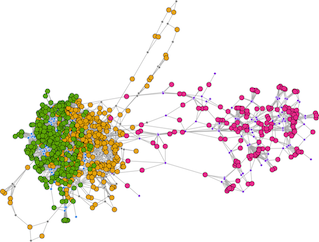
\includegraphics[scale=.4]{plots/image_SBM.png}
\end{center}


\bigskip

Les réseaux peuvent représenter des
\begin{itemize}
\item relations sociales (amitié, connaissance, professionnelles),
\item échanges,
\item inventaires,
\item ...
\end{itemize}

\bigskip

Les réseaux peuvent \^etre ou non bipartites :  les interactions peuvent avoir lieu exclusivement entre des n\oe uds appartenant à deux groupes fonctionnels différents.


%illustration reseau

\end{frame}


\begin{frame}
 \frametitle{Terminologie}
 
 Un réseau est constitué de :
 \begin{itemize}
  \item n\oe uds / sommets qui représentent des individus / acteurs qui interagissent ou non,
  \item liens / ar\^etes / connexions qui représentent les interactions entre les paires de n\oe uds (dyade).
  
 \end{itemize}

\bigskip
 
Un réseau peut \^etre 
\begin{itemize}
  \item dirigé / orienté (e.g. échange),
  \item symétrique / non-dirigé (e.g. amitié),
  \item avec ou sans boucle.
 \end{itemize}

 Cette distinction a un sens uniquement pour les réseaux simples (pas bipartite).
 
 
\end{frame}



\begin{frame}
 \frametitle{Données disponibles et but}
 
 
\begin{center}
 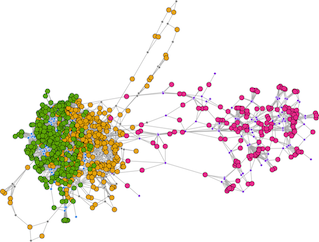
\includegraphics[scale=.4]{plots/image_SBM.png}
\end{center}

\bigskip
\textbf{Données:}
\begin{itemize}
 \item  Le réseau est fourni par:
\begin{itemize}
 \item une matrice d'adjacence (réseau simple) ou une matrice d'incidence (réseau bipartite),
 \item une liste de dyades connectés (c'est-à-dire toutes les ar\^etes). Il est sous entendu que les dyades non mentionnés ne sont pas connectées...
\end{itemize}

\item des covariables additionnelles sur les n\oe uds ou sur les dyades.
 \end{itemize}



\bigskip


\textbf{Buts:}
\begin{itemize}
 \item Révéler / décrire / modéliser la topologie du réseau. 
 \item Découvrir des structures d'interactions particulières entre des sous-parties du réseau.
 \item Comprendre l'hétérogénéité du réseau.
 \item Pas d'inférer le réseau!
 \end{itemize}


\end{frame}




\begin{frame}
\frametitle{Représentation du réseau}

 \begin{columns}
 \begin{column}{.35\paperwidth}
Matrice d'adjacence : 
 $$X=\left(
\begin{array}{rrrrr}
0 & 1 & 0 & 0 \\ 
1 & 0 & 1 & 1 \\ 
0 & 0 & 0 & 0 \\ 
1 & 1 & 0 & 0 \\ 
\end{array}\right)
$$
\end{column}

\begin{column}{.2\paperwidth}
Liste d'ar\^etes (si dirigé attention à l'ordre...)
$$\left(
\begin{array}{rr}
1 & 2\\ 
1 & 4\\ 
2 & 3 \\ 
2 & 4\\ 
\end{array}\right)
$$ 
\end{column}


\begin{column}{.5\paperwidth}

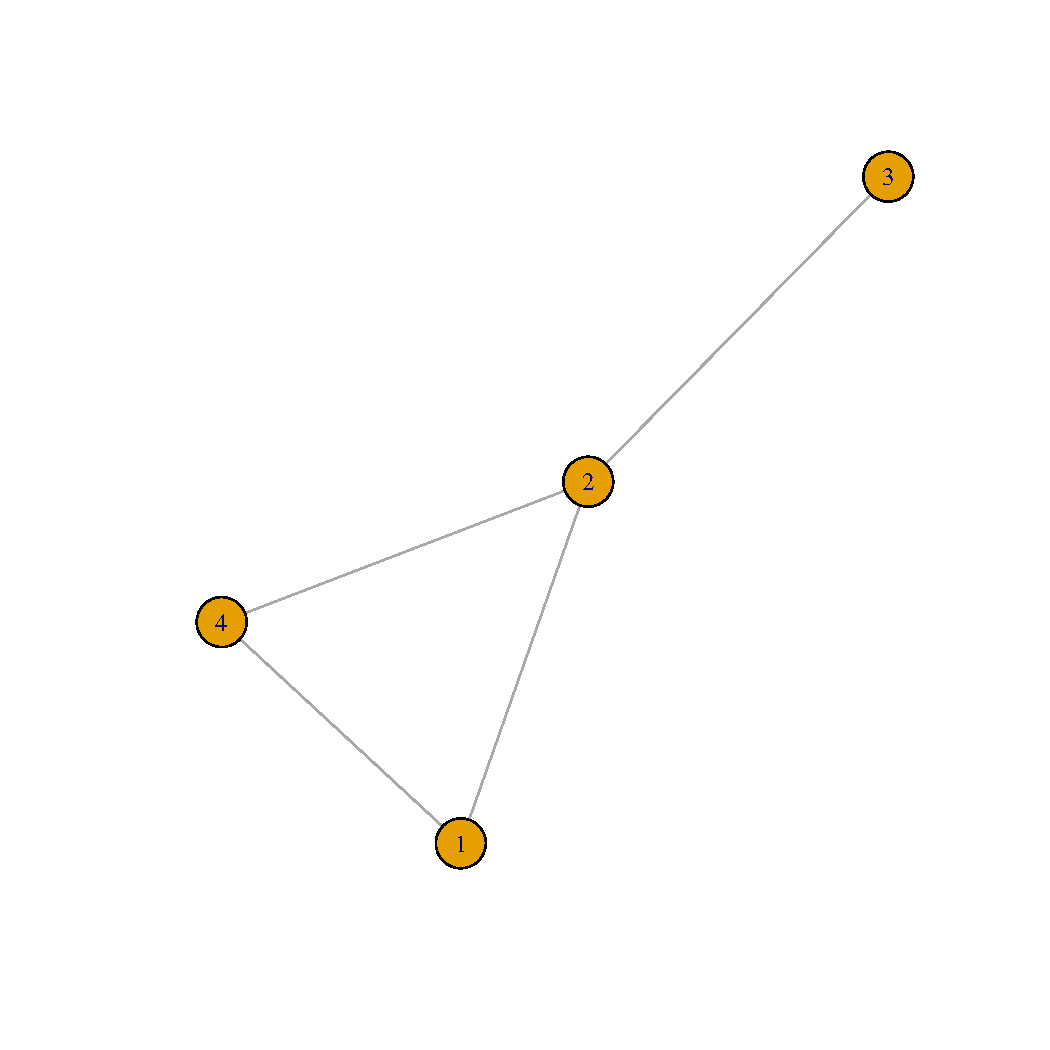
\includegraphics[scale=.3]{plots/graphe_adj.pdf}

\end{column}

\end{columns}

\begin{itemize}
\item $n$ lignes et $n$ colonnes,
\item réseau non dirigé = matrice d'adjacence symétrique.
\end{itemize}

\end{frame}

\begin{frame}
\frametitle{Réseau bipartite}
 \begin{columns}
 \begin{column}{.35\paperwidth}
Matrice d'incidence
 $$X=\left(
\begin{array}{rrrrrrr}
  0 &   1 &   1 &   0 &   1 &   0 &   0 \\ 
  0 &   0 &   0 &   1 &   0 &   1 &   1 \\ 
  0 &   0 &   0 &   0 &   1 &   0 &   0 \\ 
  0 &   1 &   0 &   0 &   0 &   0 &   1 \\ 
\end{array}\right)
$$


\begin{itemize}
 \item n lignes et m colonnes, matrice rectangulaire.
 \item matrice d'adjacence correspondante $(n+m)\times(n+m)$:
 $$
 \left(
 \begin{array}{rr}
  0 & X\\
  X^T & 0
 \end{array}
 \right)
 $$
\end{itemize}

\end{column}

 \begin{column}{.2\paperwidth}
  Liste d'ar\^etes : 
 $$\left(
 \begin{array}{rr}
 A1 & B2 \\ 
 A1 & B3 \\ 
 A1 & B5 \\ 
 A2 & B4 \\ 
 A2 & B6 \\ 
 A2 & B7 \\ 
 A3 & B5 \\ 
 A4 & B2 \\ 
 A4 & B7 \\   
 \end{array}
 \right)$$ 
  
 \end{column}


\begin{column}{.3\paperwidth}

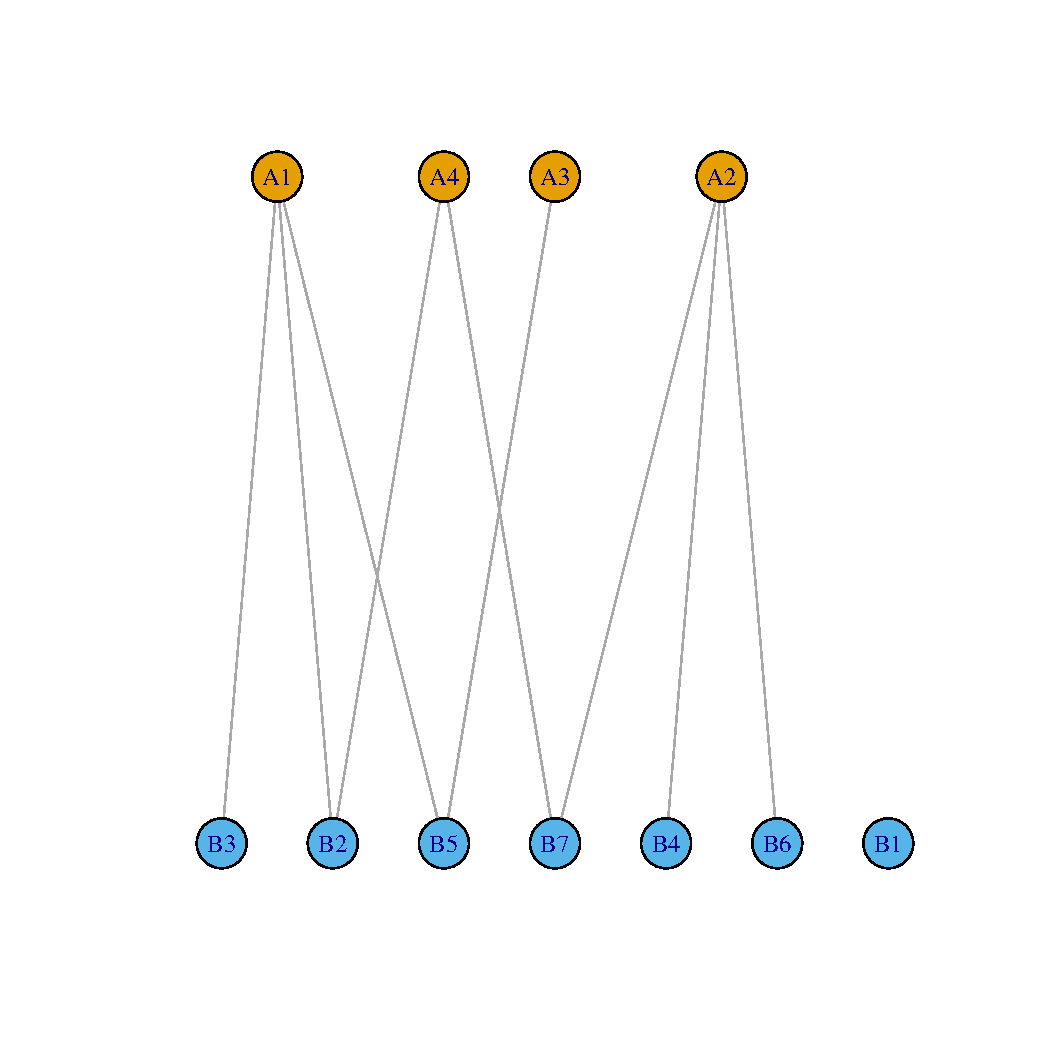
\includegraphics[scale=.25]{plots/graphe_bipartite.pdf}

\end{column}

\end{columns}



\end{frame}




\section{Représentation des réseaux}

\begin{frame}
 \frametitle{Différentes représentations possibles : au hasard}
 
 \begin{center}
 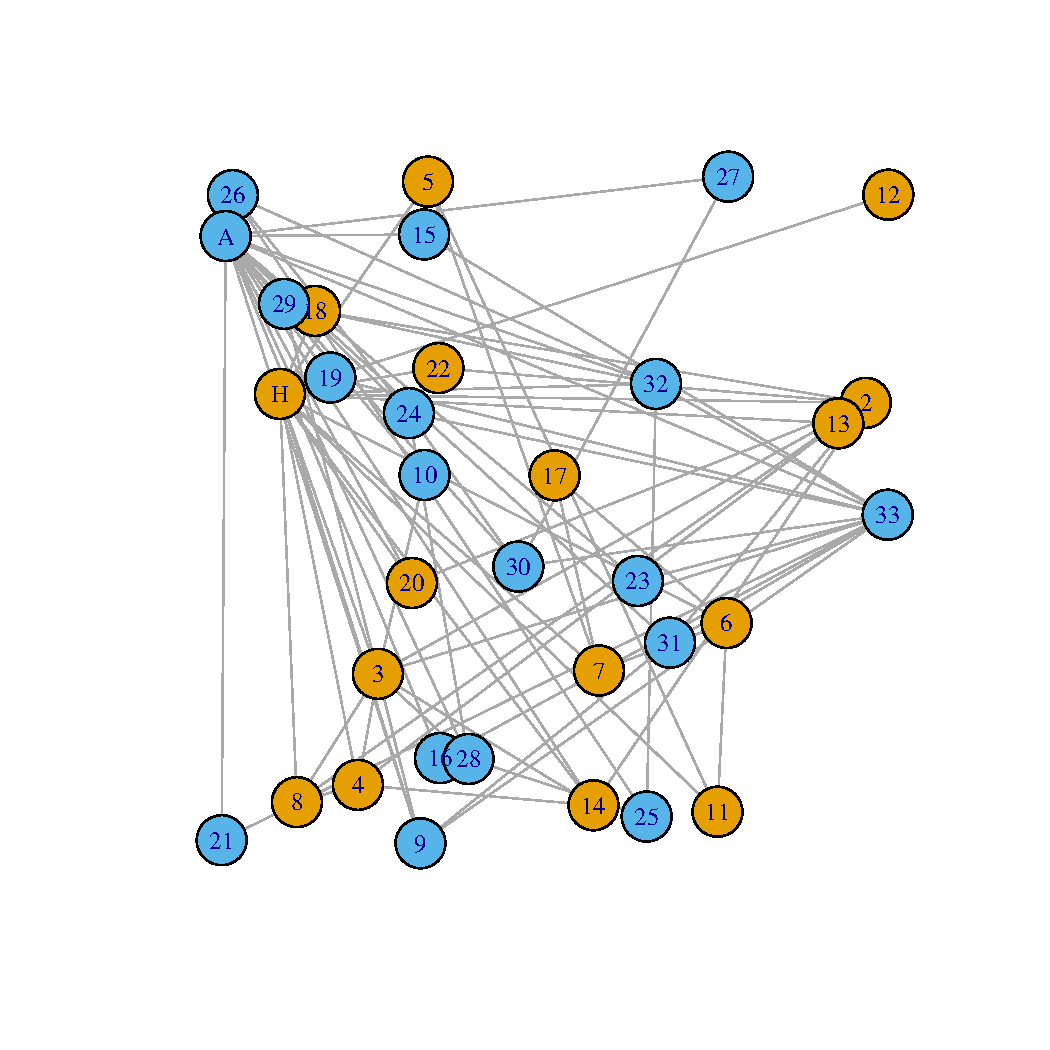
\includegraphics[scale=.3]{plots/karateRandom1.pdf}
  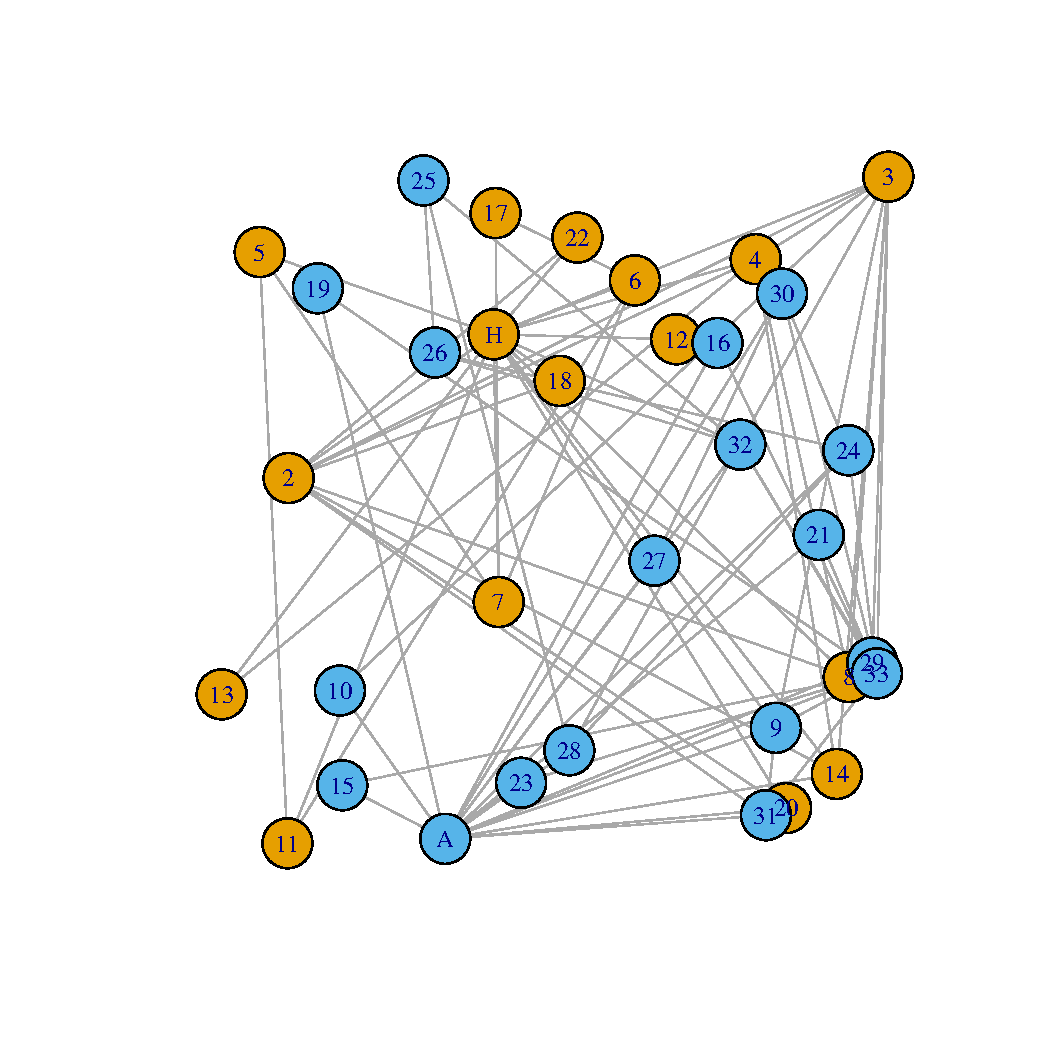
\includegraphics[scale=.3]{plots/karateRandom2.pdf}
  
 \end{center}
 
\end{frame}



\begin{frame}
 \frametitle{Fruchterman–Reingold}
 Ar\^etes de longueurs à peu près égales et peu de croisement. Mais représentations différentes à chaque appel.
 
 
  \begin{center}
 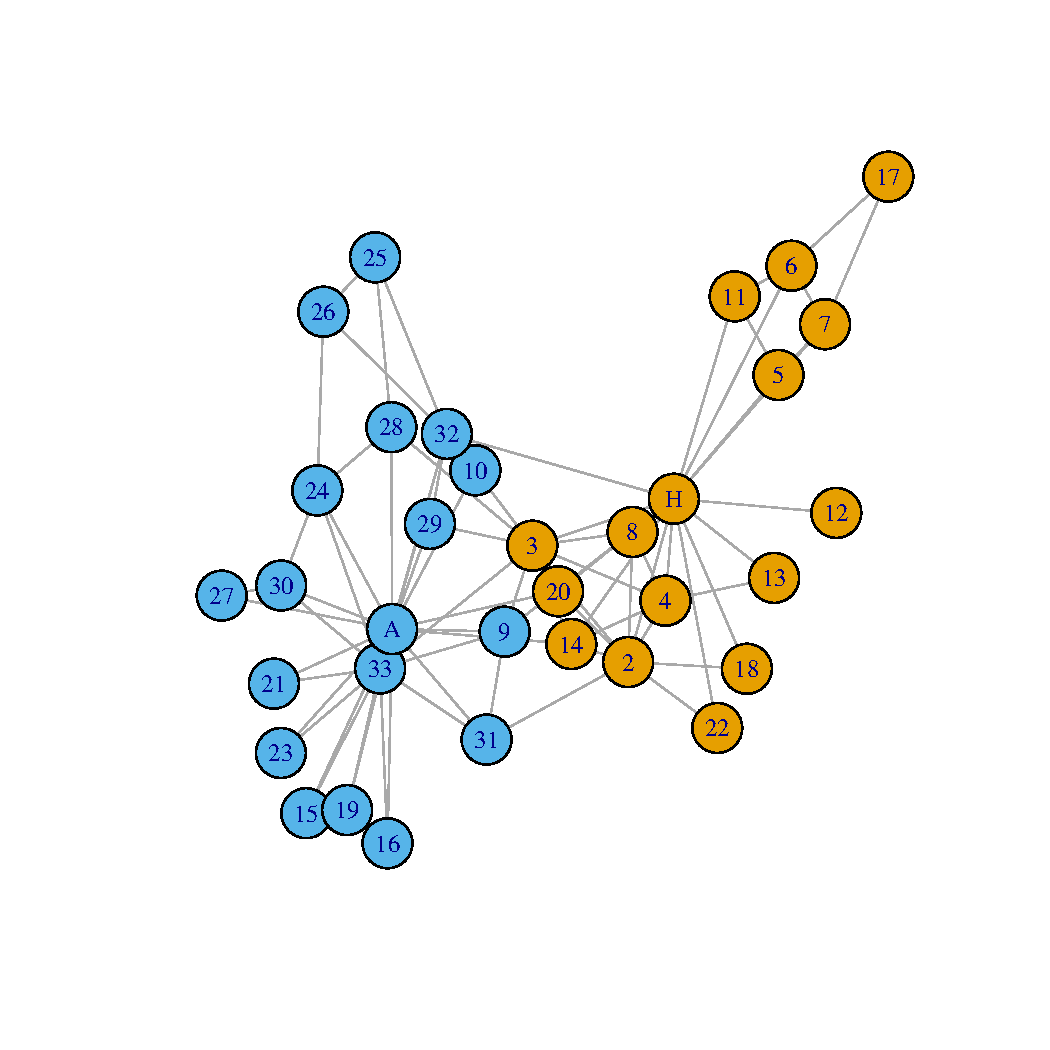
\includegraphics[scale=.3]{plots/karateFR1.pdf}
  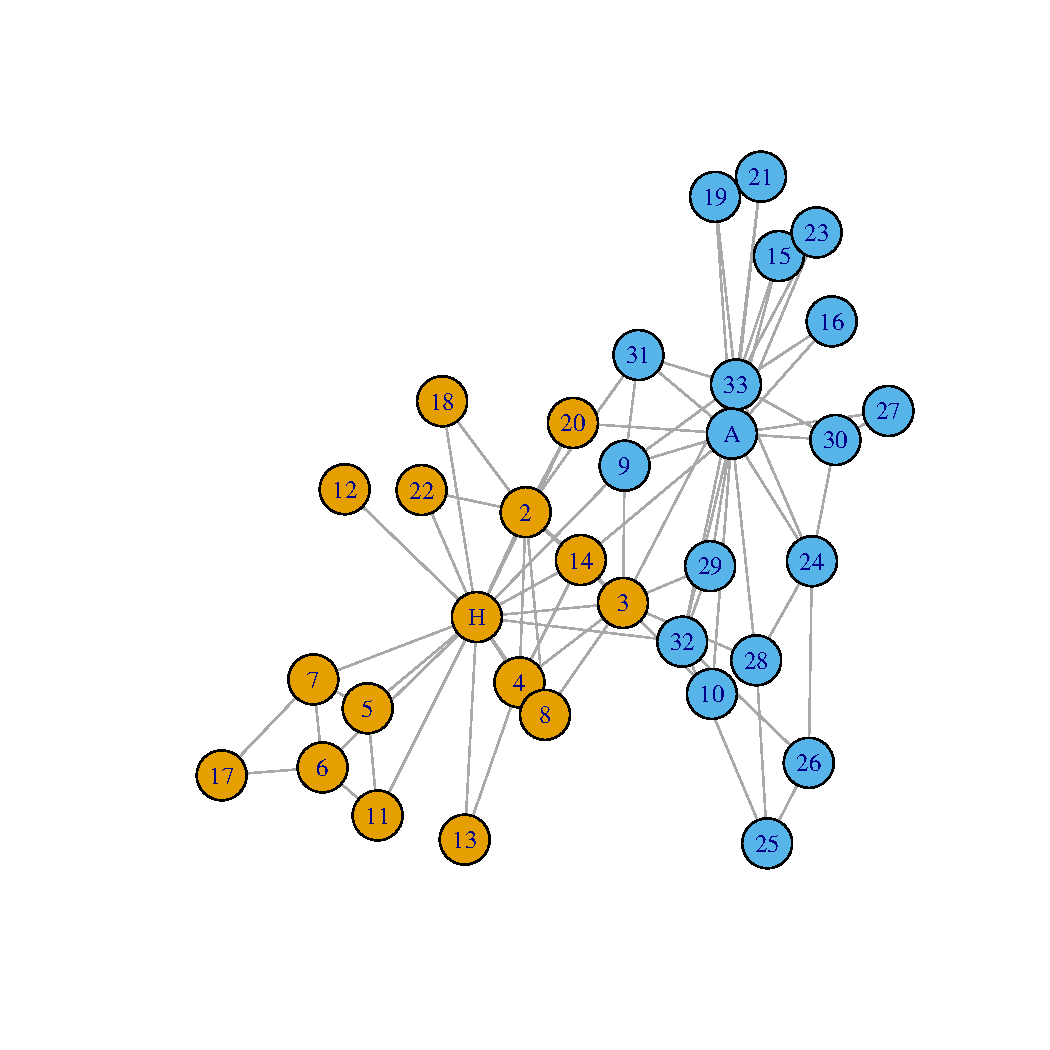
\includegraphics[scale=.3]{plots/karateFR2.pdf}
  
 \end{center}
 
\end{frame}




\begin{frame}
 \frametitle{Autres représentations}
 
 \begin{columns}
  \begin{column}{.45\paperwidth}
   Graphe dirigé
   
   \centering
     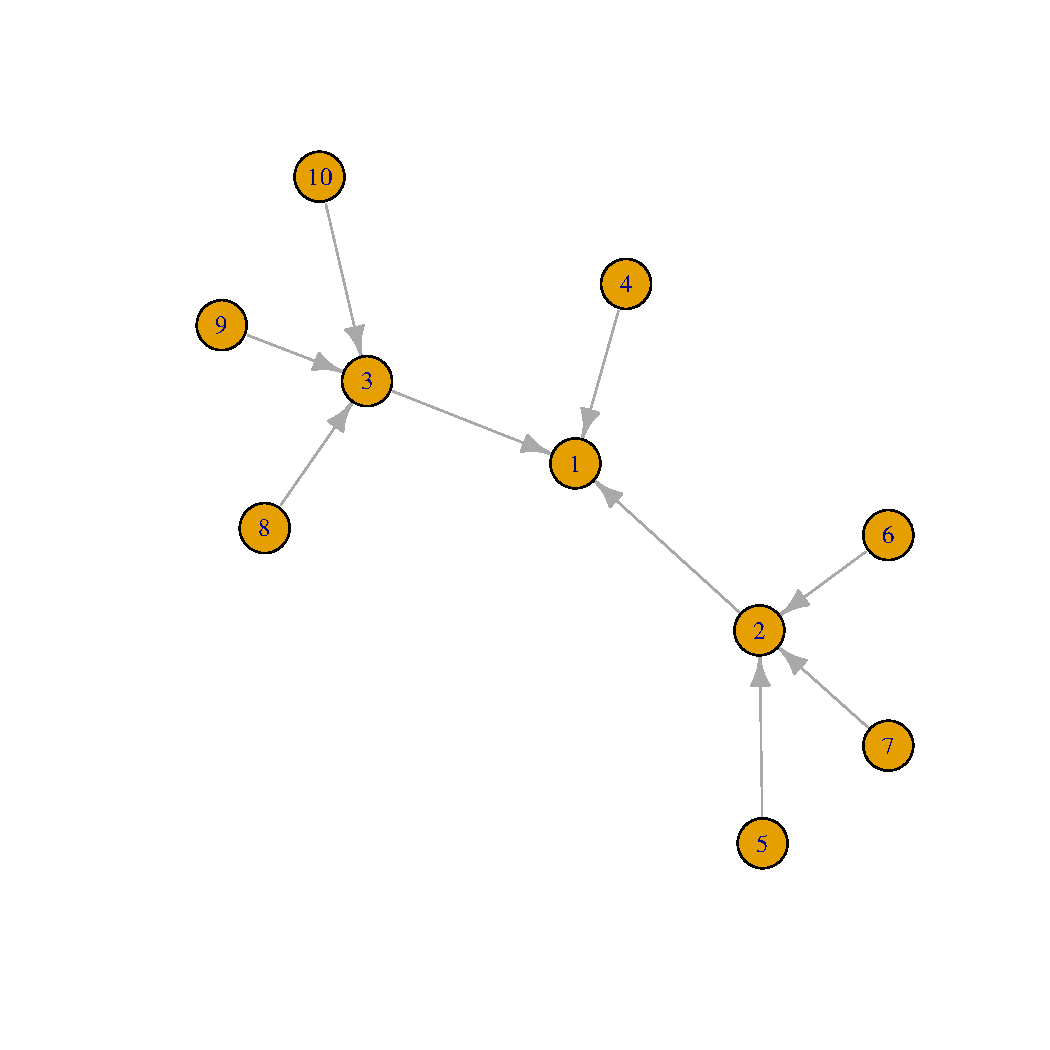
\includegraphics[scale=.3]{plots/arbredirige.pdf}
  \end{column}
 \begin{column}{.45\paperwidth}
   Graphe bipartite
   
    \centering
     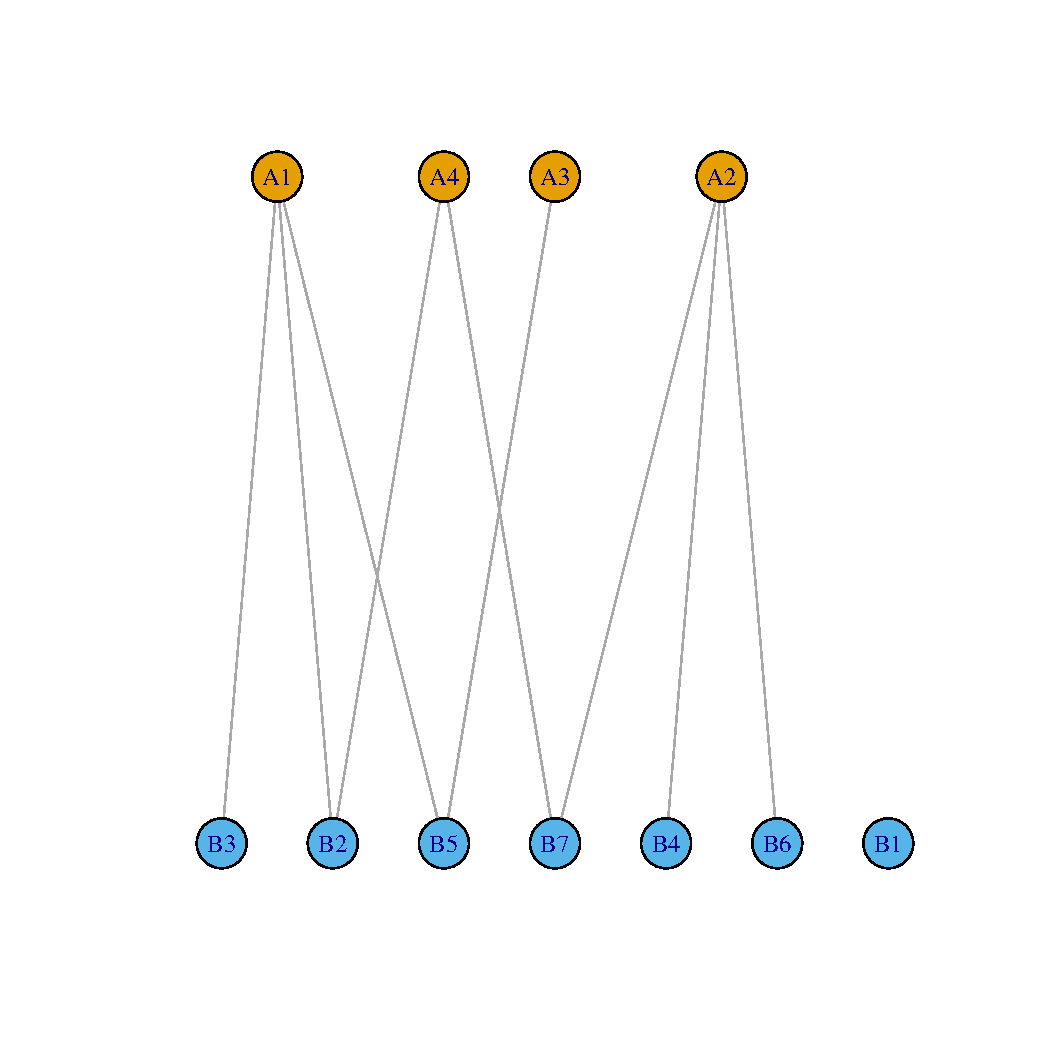
\includegraphics[scale=.3]{plots/graphe_bipartite.pdf}
  \end{column}
 \end{columns}

 
\end{frame}




\section{Statistiques résumées simples}

\begin{frame}
\frametitle{Quelques statistiques résumées simples}


% ref a mettre et sans doute à partager en plusieurs slides à la siute
\begin{itemize}

\item Degrés, sortant ou entrant si dirigés :
\begin{eqnarray*}
 \overrightarrow{D}_i&=&\sum_j X_{ij}\\
 \overleftarrow{D}_j&=&\sum_i X_{ij}
\end{eqnarray*}

\item Nestedness: si les n\oe uds de plus petit degré se connectent aux n\oe uds de plus haut degré,
\textcolor{blue}{Rodríguez-Gironés \& Santamaria (2006)}

\item Centralité (betweenness): pour un n\oe ud, nombres de chemins les plus courts entre n'importe quelle paire de n\oe uds passant par ce n\oe ud.
\textcolor{blue}{Freeman (1979)}

\item Modularité: mesure pour une partition de sa tendance à favoriser l'intra-connexion par rapport à l'inter-connexion.
$\Rightarrow$ Recherche de la meilleure partition. 
\textcolor{blue}{Clauset, Newman \& Moore (2004)}
\end{itemize}


\bigskip

Critères à adapter aux
\begin{itemize}
 \item réseaux dirigés,
 \item réseaux bipartites.
\end{itemize}

\bigskip

%\textcolor{blue}{R packages: igraph, sna, vegan.} 


\end{frame}



\begin{frame}
 \frametitle{Example Chilean food web}
 
\begin{center}
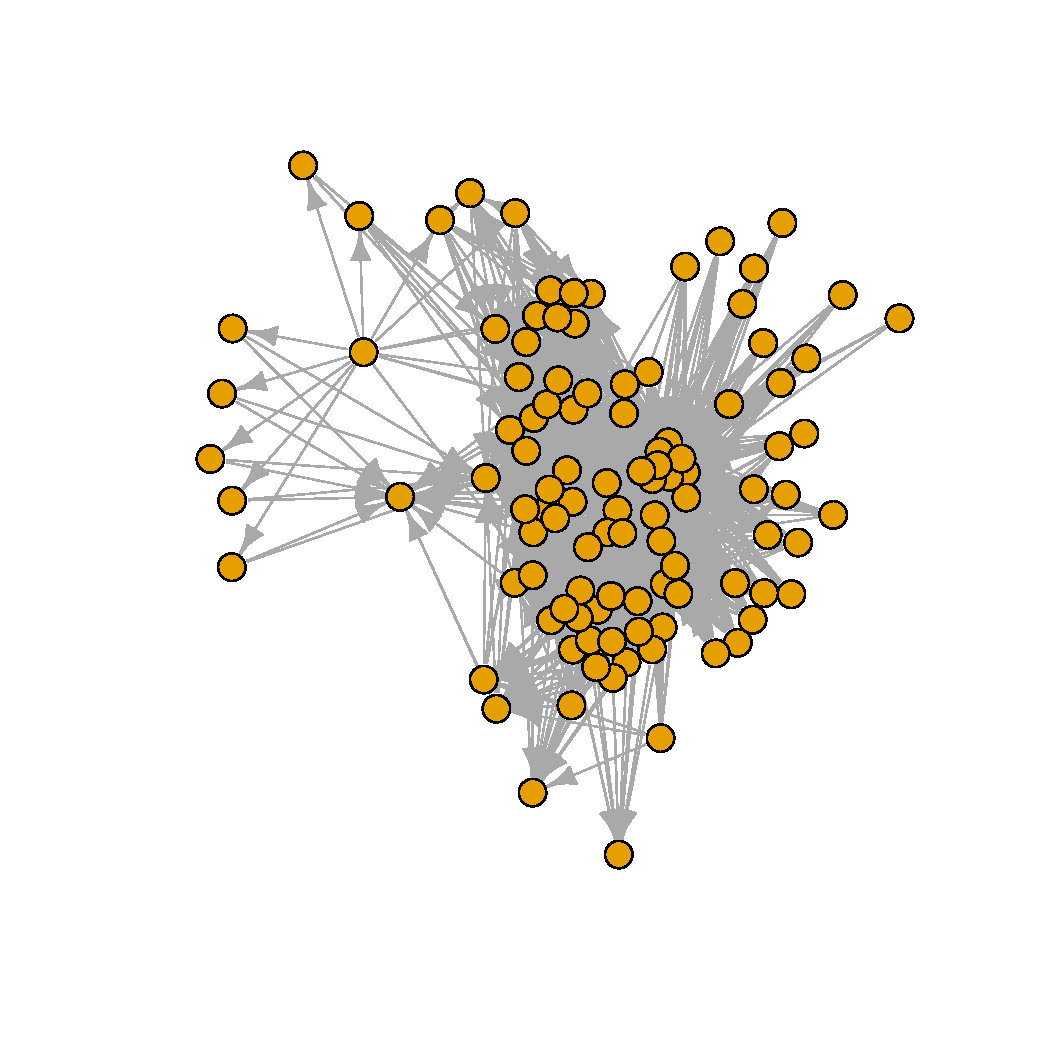
\includegraphics[scale=.3]{plots/chilean_food_web.pdf} 
\end{center}

\begin{itemize}
 \item $n=106$ espèces / n\oe uds,
 \item densité: $12.1\%$.
\end{itemize}


\textcolor{blue}{Kéfi, Miele, Wieters, Navarrete \& Berlow (2016)}

\end{frame}


\begin{frame}
 \frametitle{Distribution des degrés}
 
 \begin{center}
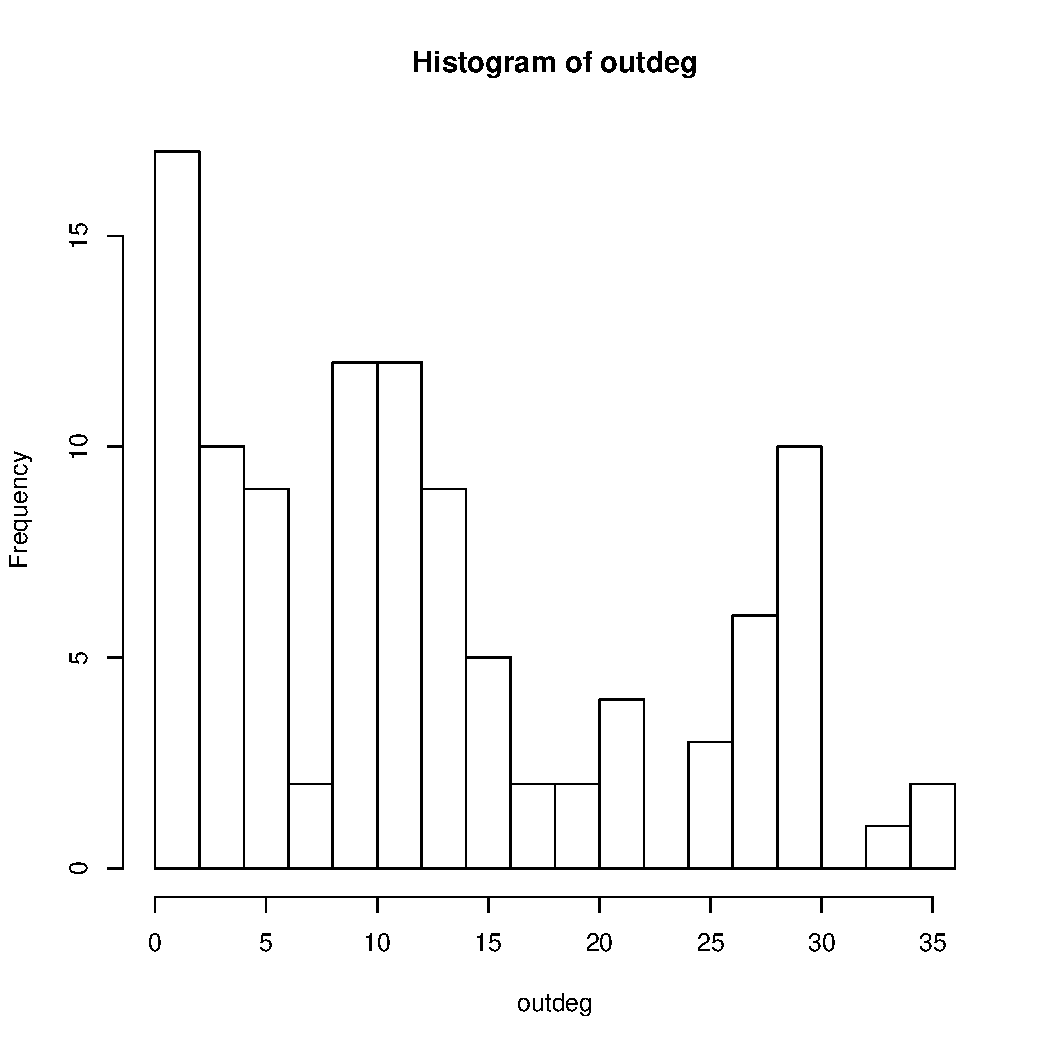
\includegraphics[scale=.3]{plots/chilean_outdeg.pdf}  
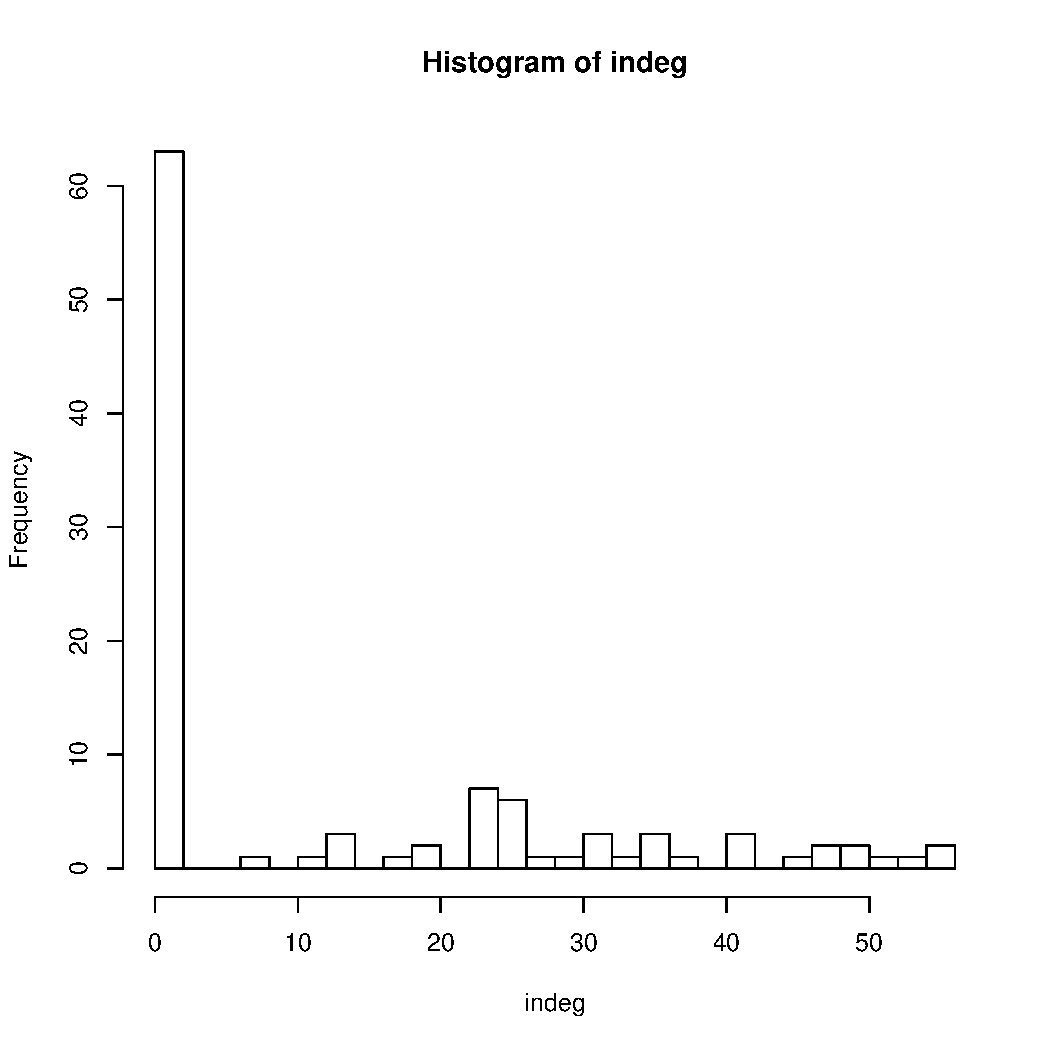
\includegraphics[scale=.3]{plots/chilean_intdeg.pdf}
\end{center}

\end{frame}


\begin{frame}
 \frametitle{Nestedness}
 
 \begin{center}
  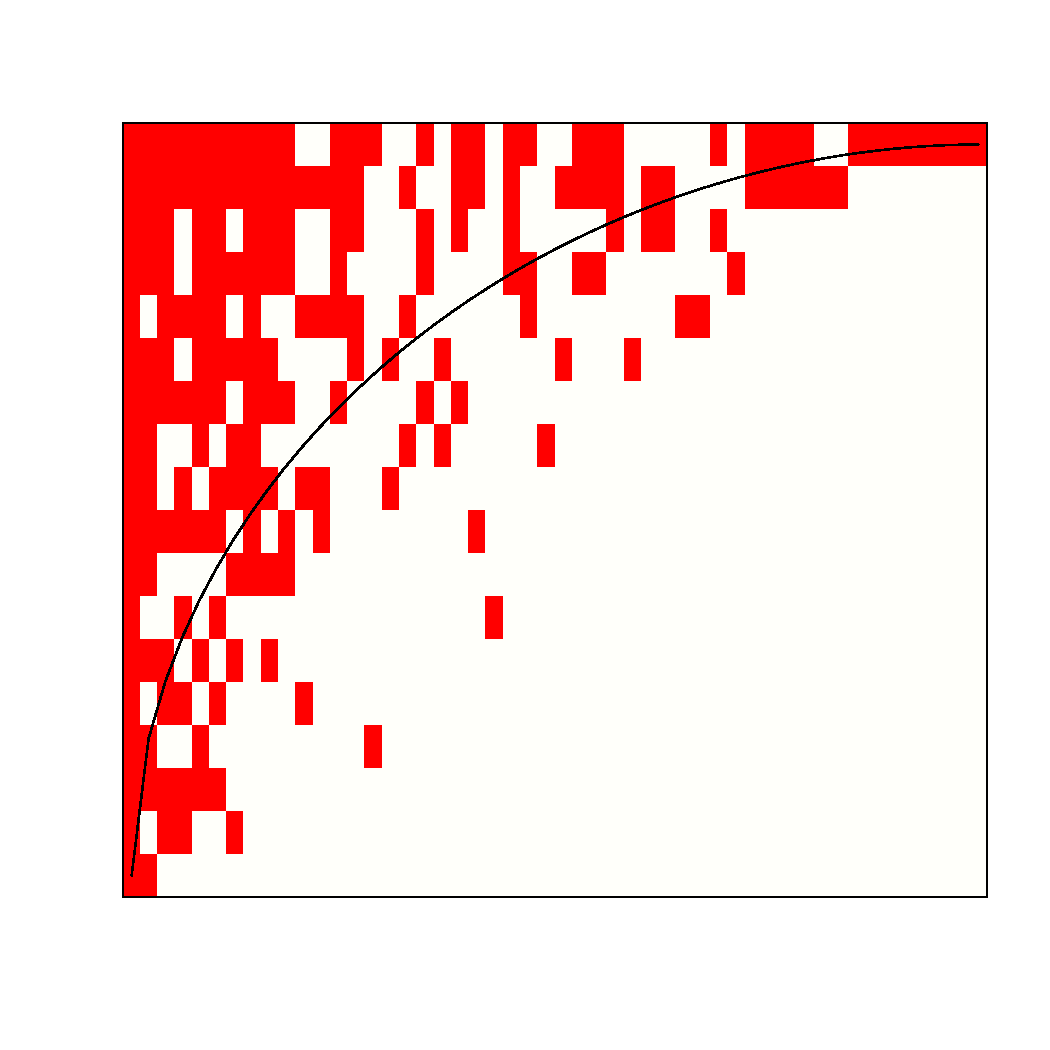
\includegraphics[scale=.3]{plots/chilean_nested.pdf}
 \end{center}


 \begin{itemize}
  \item plus généralement sur les graphes bipartites,
%  \item significance of the nestedness index computed by random permutations of the matrix,
  \item ce réseau est trouvé embo\^ité.
 
 \end{itemize}

 \end{frame}


\begin{frame}[fragile]
 \frametitle{Centralité (Betweenness)}
 
 \begin{center}
  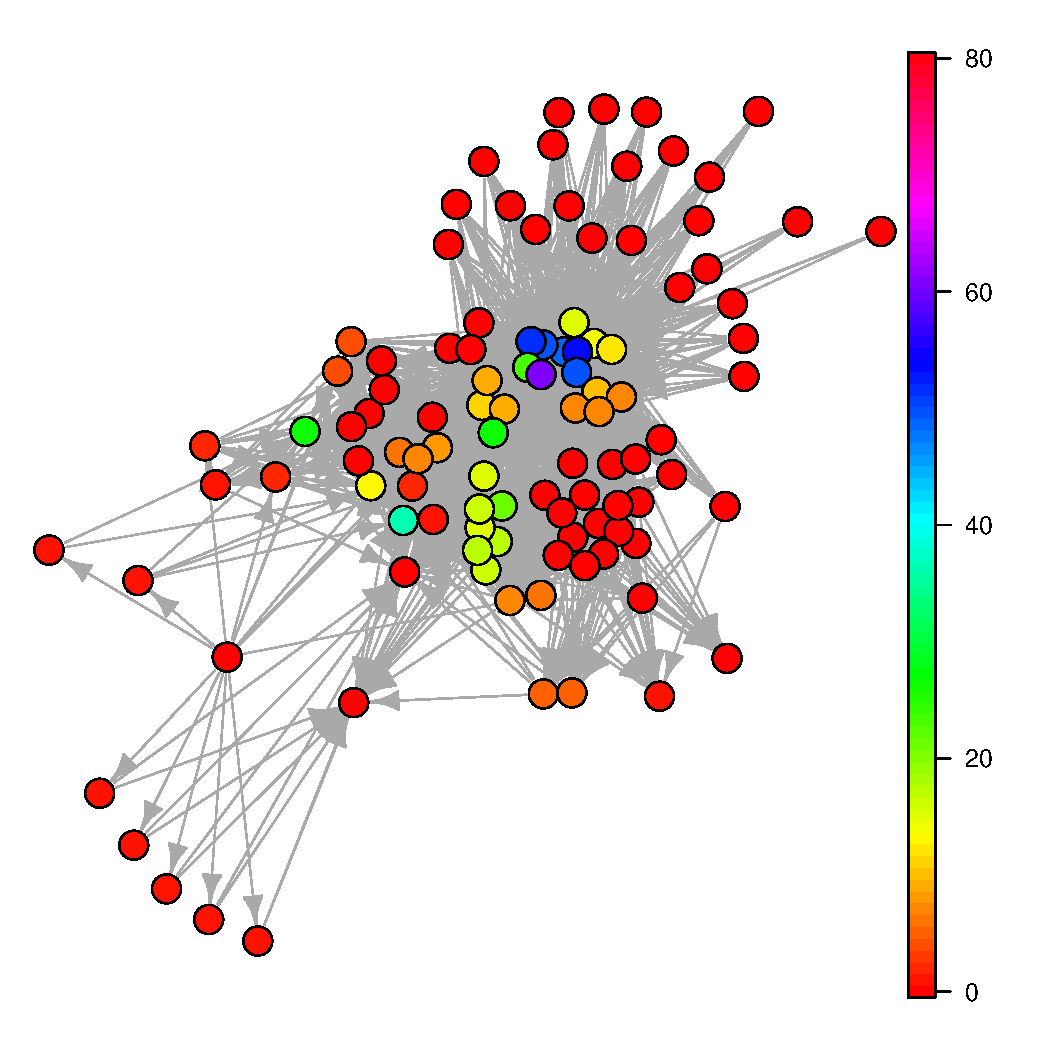
\includegraphics[scale=.3]{plots/chilean_between.pdf}
 \end{center}

\begin{verbatim}
   Min. 1st Qu.  Median    Mean 3rd Qu.    Max. 
 0.000   0.000   0.000   6.604   6.929  59.570
\end{verbatim} 
 
\end{frame}


\begin{frame}
 \frametitle{Modularité}
\begin{center}
  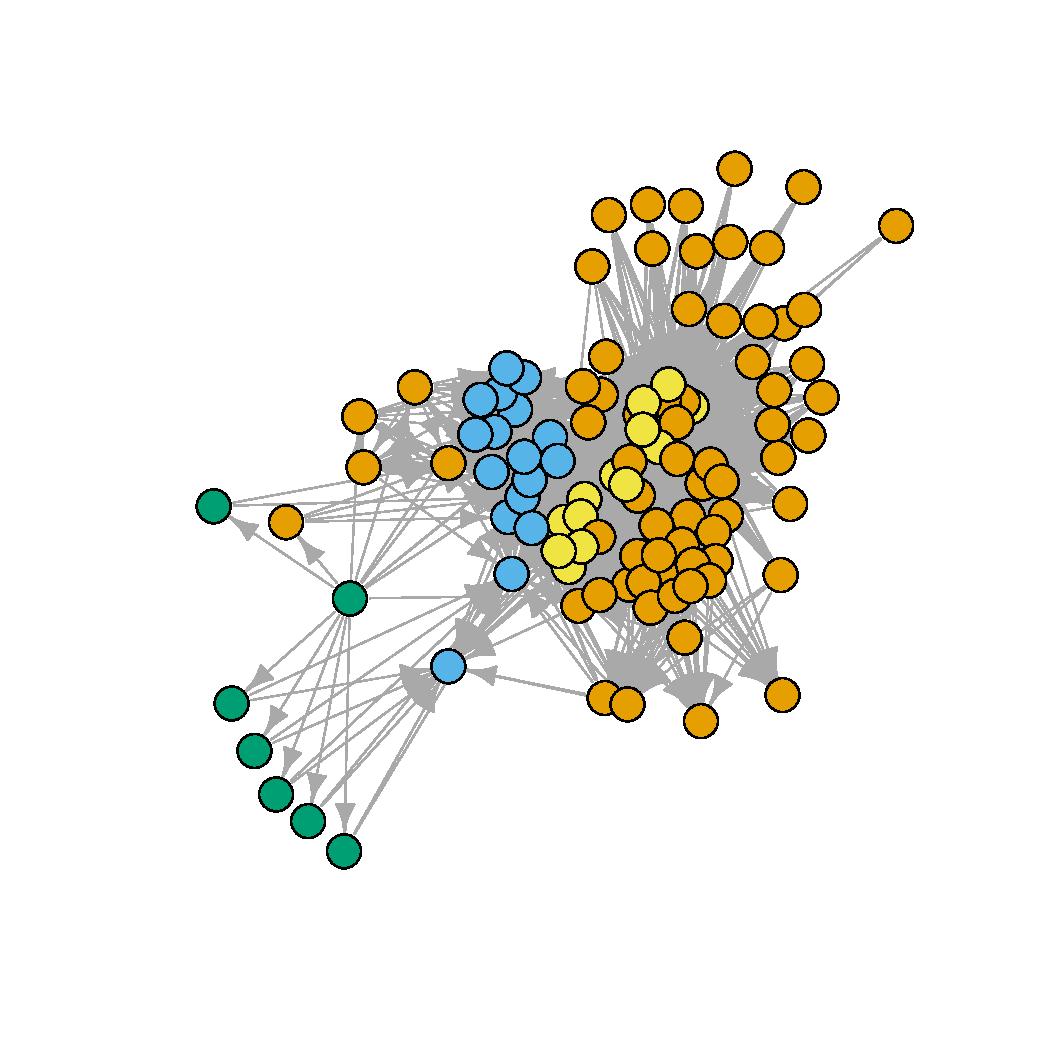
\includegraphics[scale=.3]{plots/chilean_modularity.pdf}
 \end{center}
 
 
 
 \begin{itemize}
  \item
  \begin{tabular}{rrrrr}
  \hline
 1 & 2 & 3 & 4 \\ 
  \hline
  69 &  17 &   7 &  13 \\ 
   \hline
\end{tabular}
\item modularité très faible.
 \end{itemize}

 
\end{frame}


\section{Modèles probabilistes}


\begin{frame}
 \frametitle{Modèles}
 
 
 \begin{itemize}
  \item Stochastic Block Model (SBM) pour les réseaux simples / matrices d'adjacence.
  \item Latent Block Model (LBM) pour les réseaux bipartites / matrices d'incidence.
  \item Exponential Random Graph Model pour les réseaux simples.
 \end{itemize}

\end{frame}


 
 
\begin{frame}\frametitle{Inférence du SBM} 

De...

\centering
\begin{tabular}{cc}
 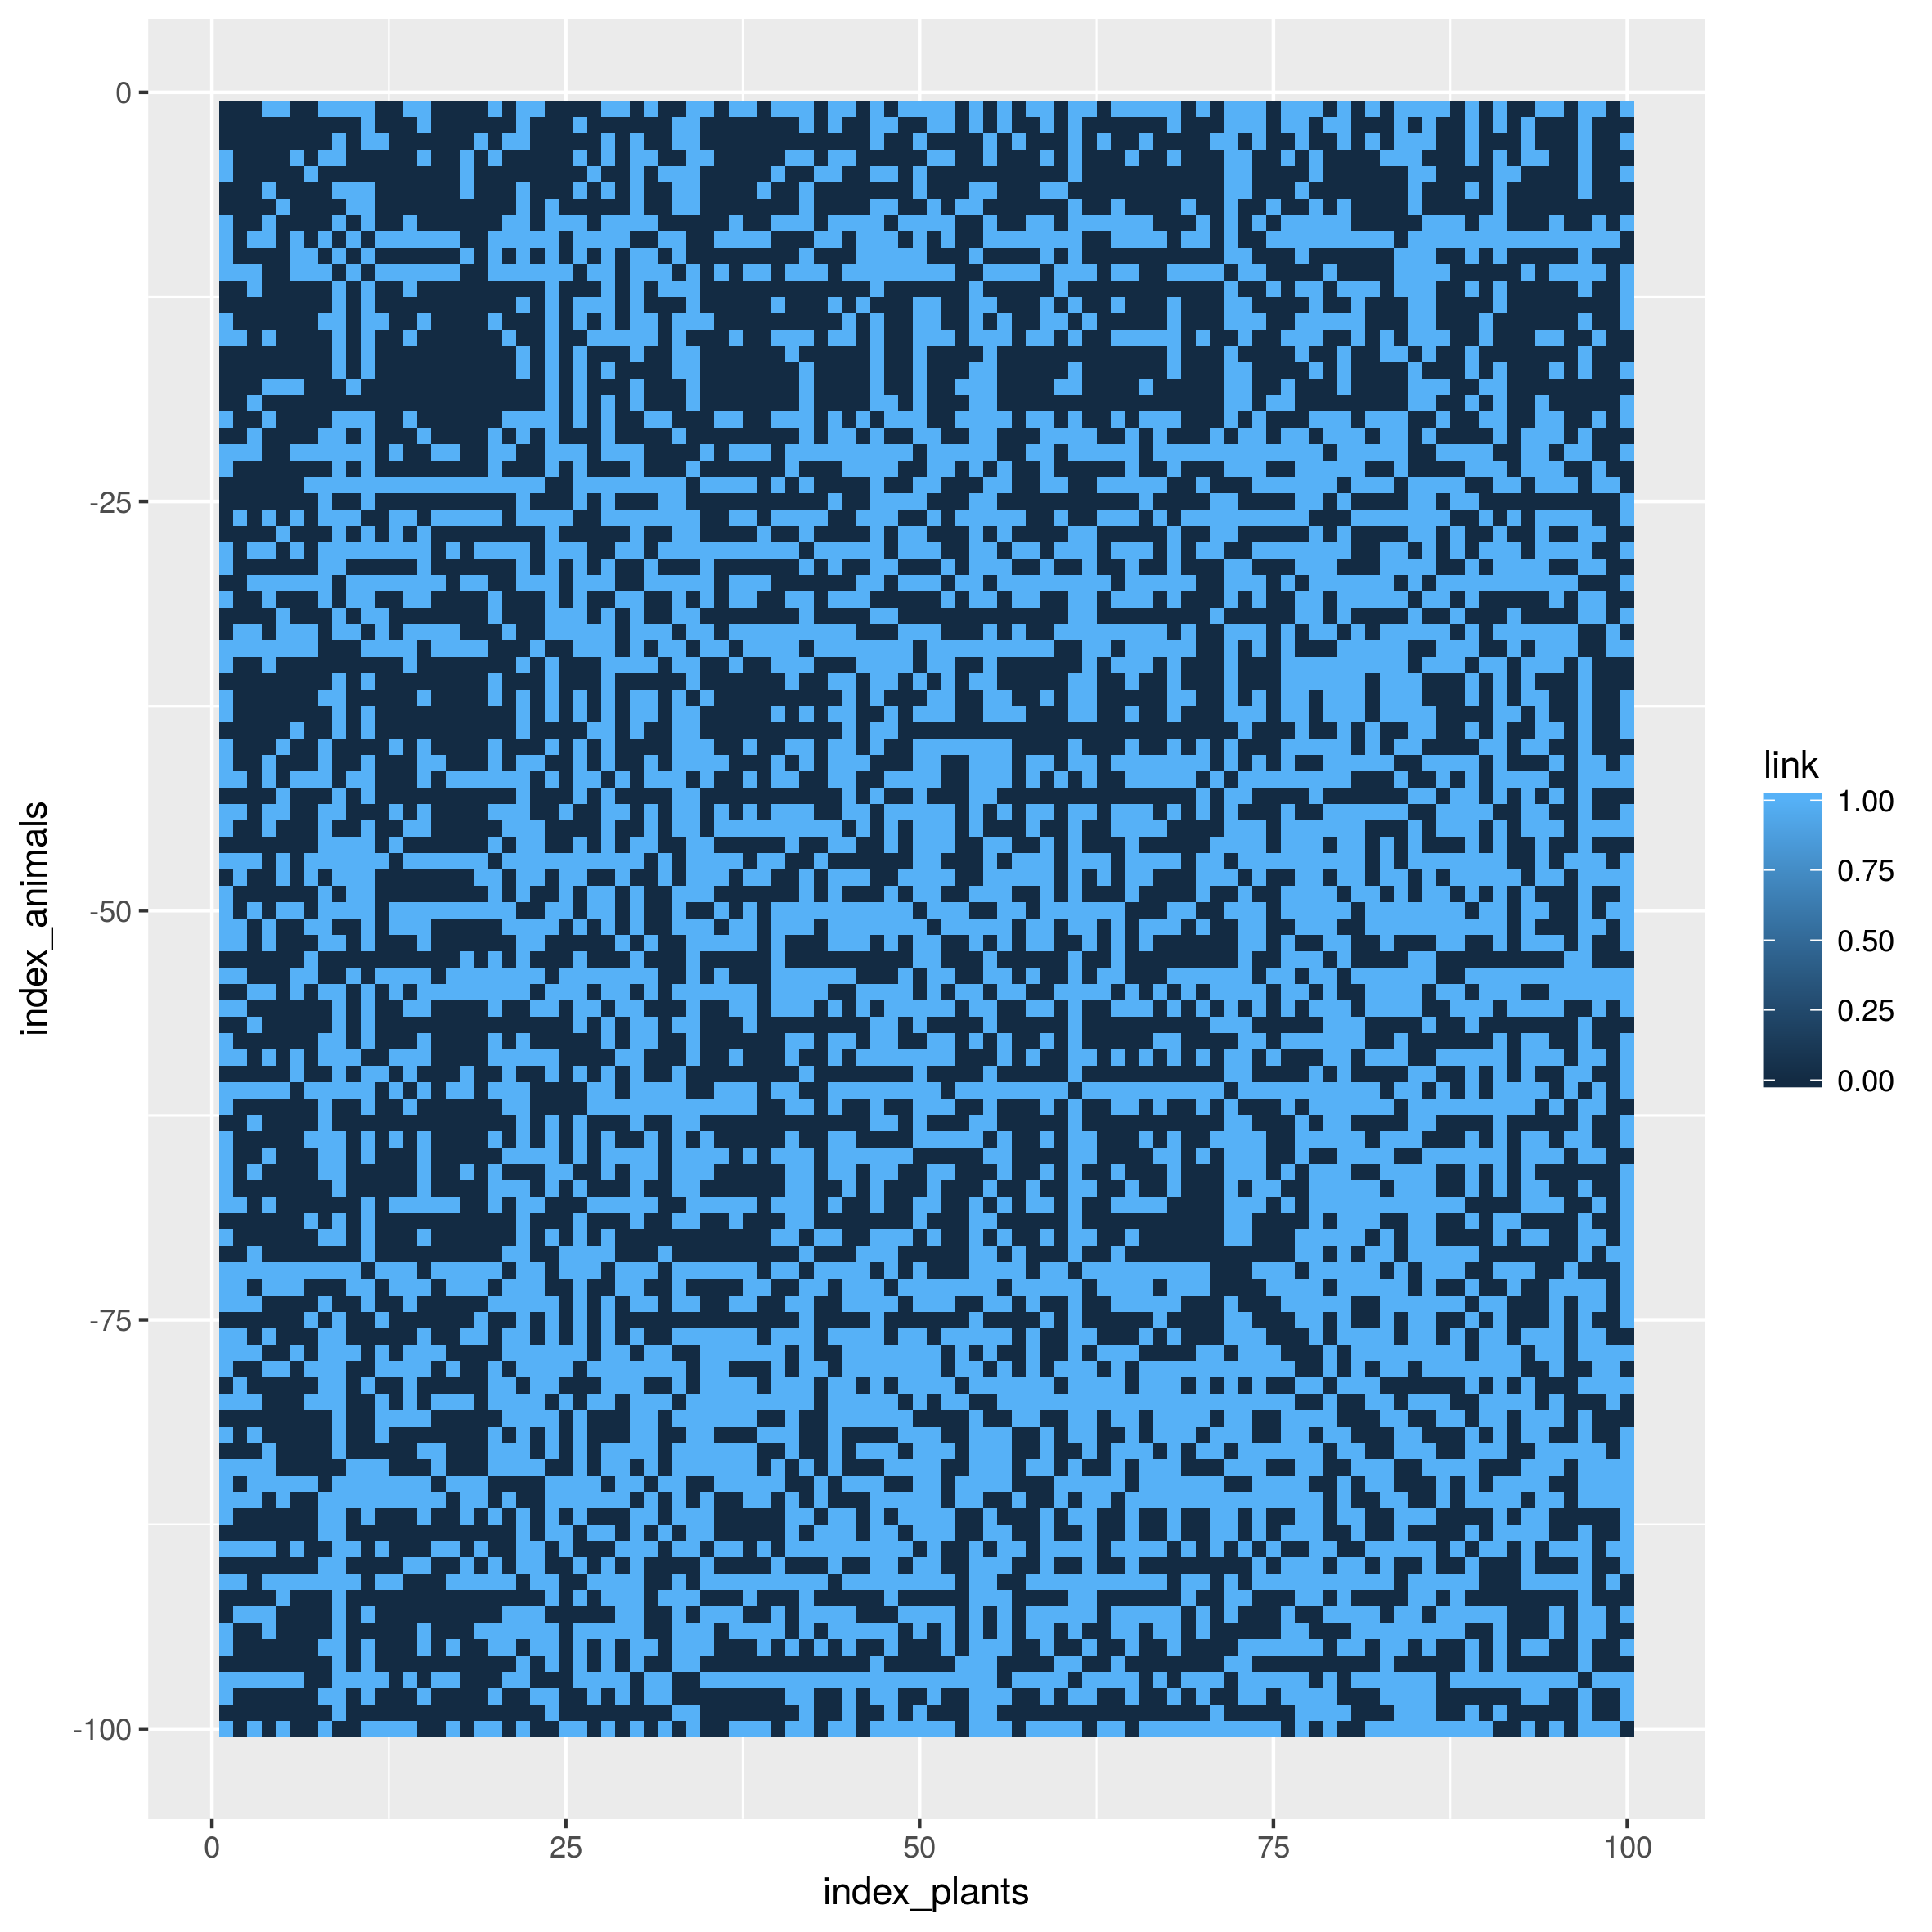
\includegraphics[scale=.2]{plots/sbm/Nested_adja.png}&
 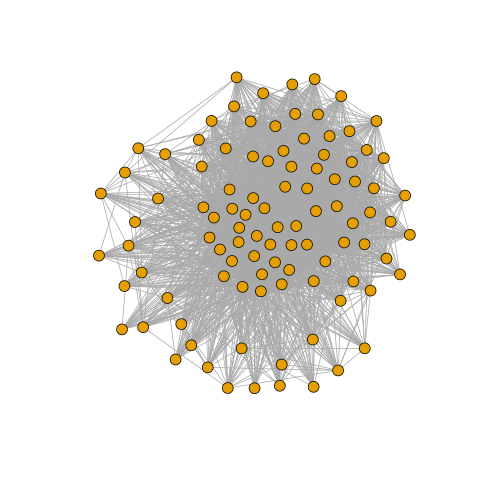
\includegraphics[scale=.2]{plots/sbm/Nested_graphe_without_colors.png}
\end{tabular}
\end{frame}

\begin{frame}\frametitle{Inférence du SBM} 

... à 

\centering
\begin{tabular}{cc}
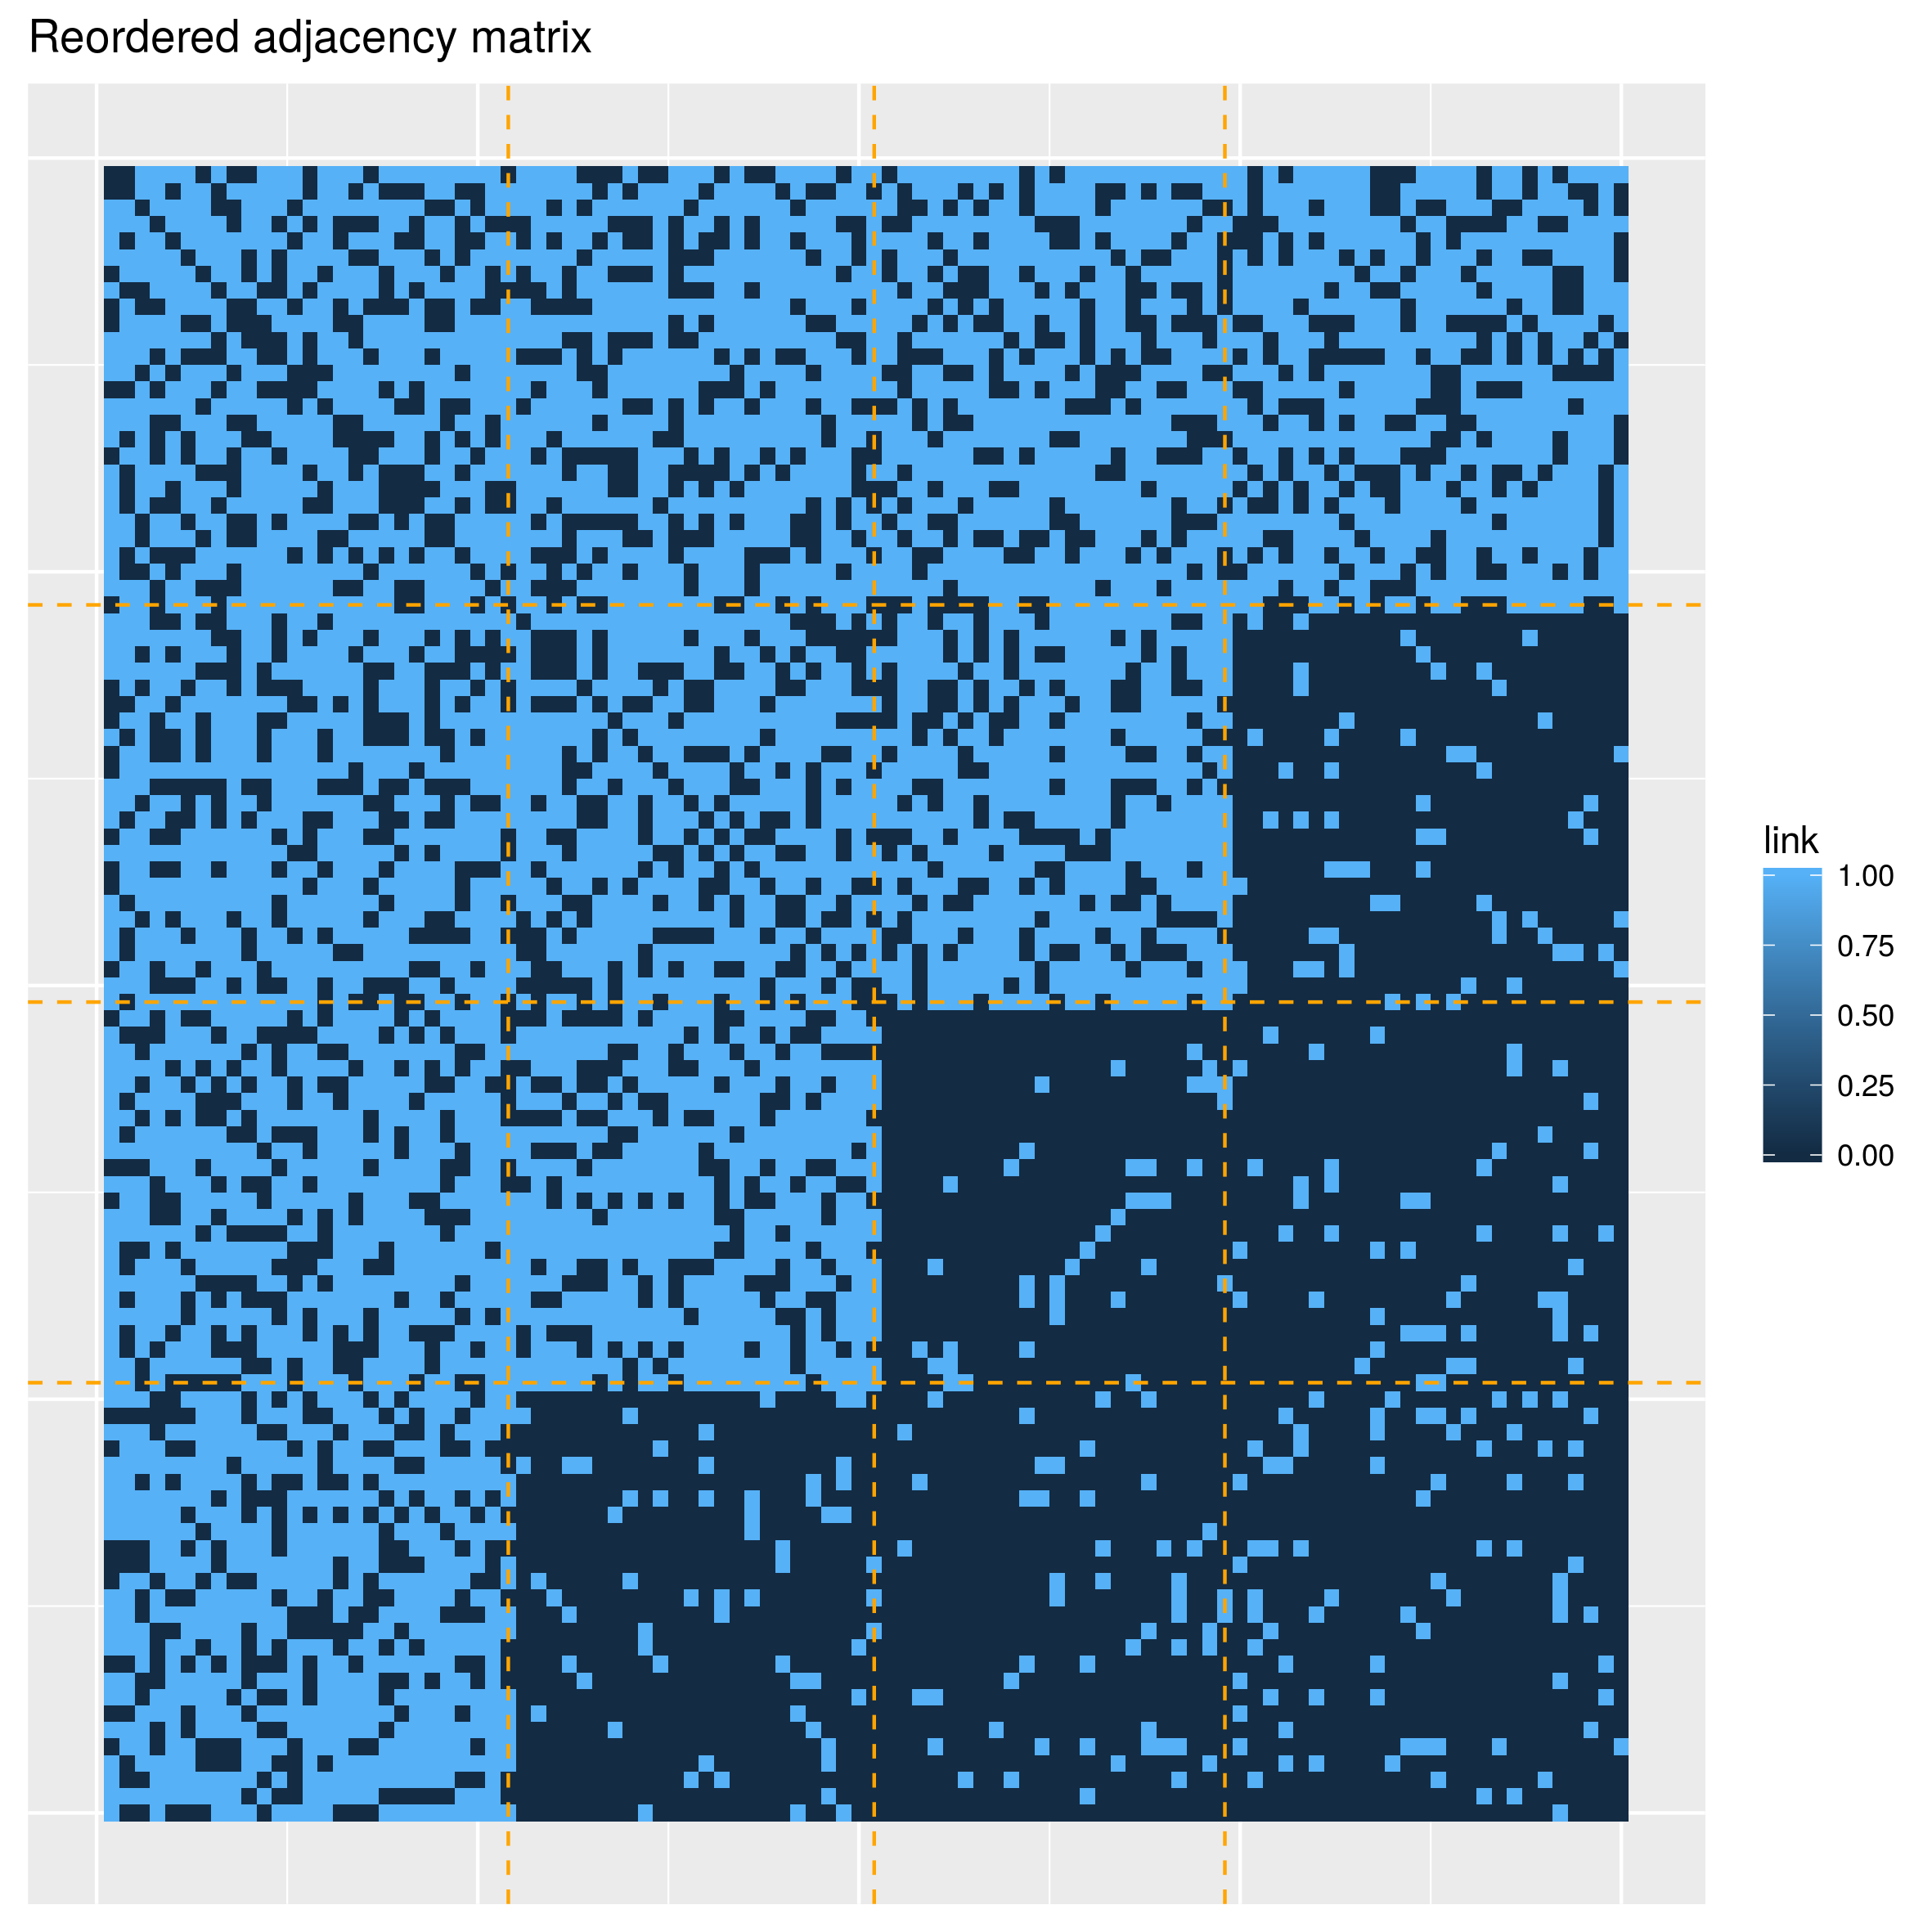
\includegraphics[scale=.2]{plots/sbm/Nested_reordered_adja_with_groups.png}
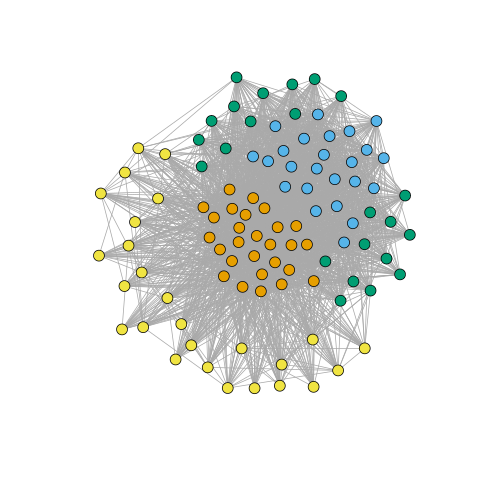
\includegraphics[scale=.2]{plots/sbm/Nested_graphe_with_colors.png}
\end{tabular}

\begin{block}{Travail statistique}
\begin{itemize}
\item Identifier les groupes
\item Trouver le nombre de cluster
\item Estimation des paramètres
\end{itemize}
\end{block}

\end{frame}



\begin{frame}
 \frametitle{Application au réseau trophique chilien }
 
 \begin{center}
  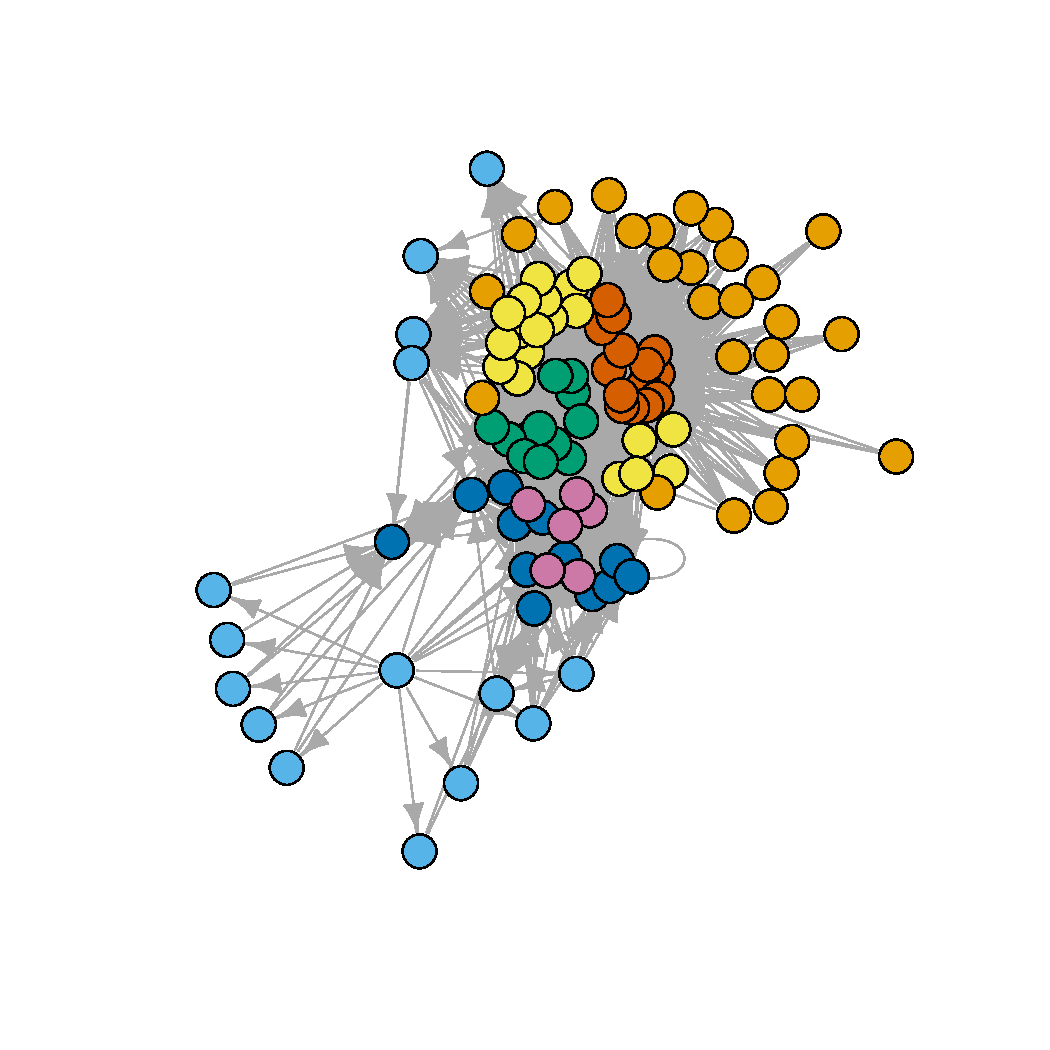
\includegraphics[scale=.3]{plots/chilean_sbm.pdf}
 \end{center}

 \begin{itemize}
 \item $7$ groupes/blocs/clusters,
 \item \begin{tabular}{rrrrrrr}
  \hline
  1 & 2 & 3 & 4 & 5 & 6 & 7 \\ 
  \hline
  28 &  15 &  12 &  19 &  12 &  14 &   6 \\ 
   \hline
\end{tabular}
\end{itemize}


\end{frame}


\begin{frame}
 \frametitle{Application au réseau trophique chilien }
 
 \begin{center}
  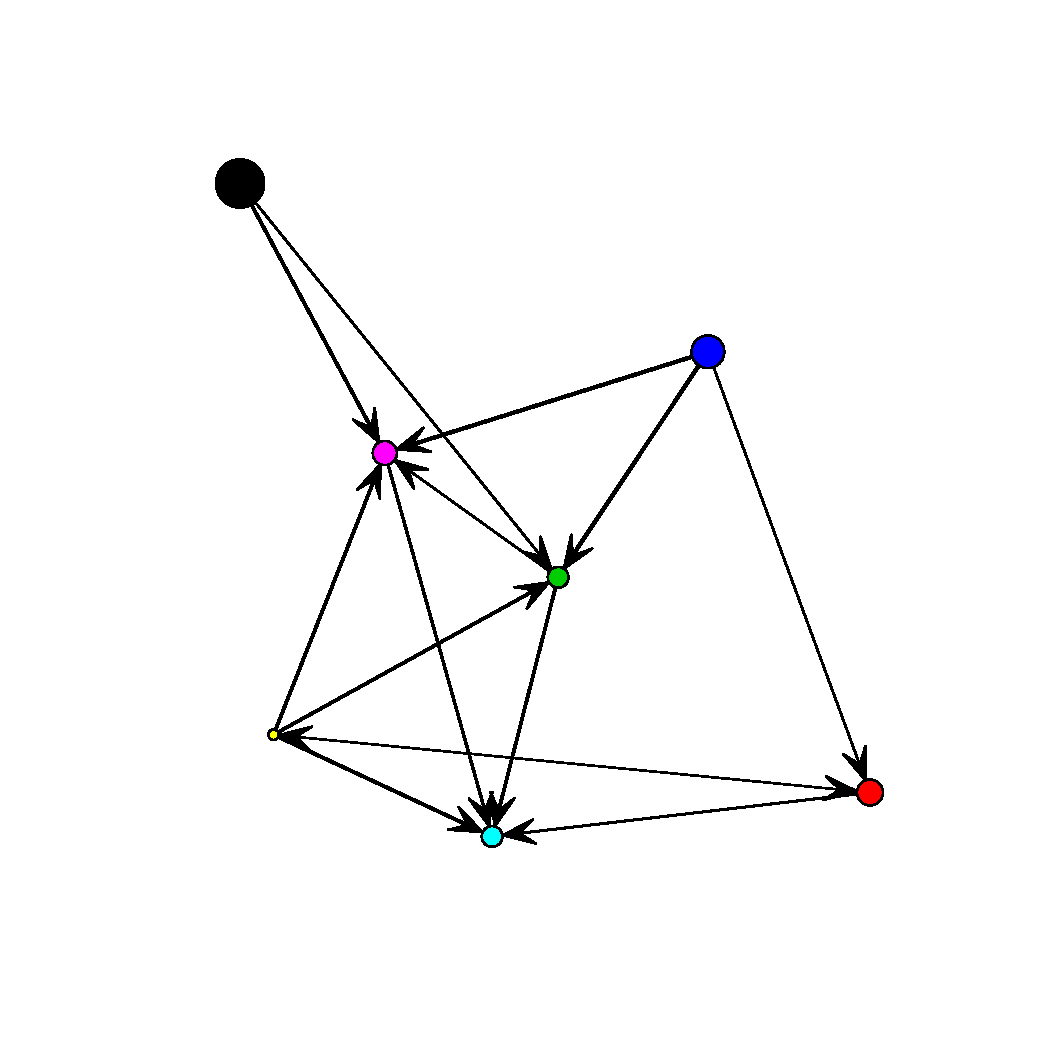
\includegraphics[scale=.3]{plots/chilean_sbm_sum.pdf}
 \end{center}

 
 
\end{frame}



\section{Covariables}


\begin{frame}
 \frametitle{Différents types de covariables}
 
 
 \begin{itemize}
  \item N\oe uds
  
  \begin{itemize}
   \item catégorielle : ethnie, village...
   \item quantitative : \^age, surface cultivée...
  \end{itemize}

  \medskip
  
  \item Dyades
  
  \begin{itemize}
   \item à partir des covariables sur les n\oe uds : différence d'\^age, \^age du donneur ou \^age du receveur,
   \item distance géographique entre les exploitations.
  \end{itemize}

  
  
 \end{itemize}

 \end{frame}

\begin{frame}
\frametitle{Analyse à l'aide des covariables}

\textbf{Interprétation : }
 
 \begin{itemize}
  \item Covariables au niveau des n\oe uds à mettre en relation avec statistiques propres au n\oe uds (degré, centralité ...)
  \item Analyser la structuration des covariables au niveau des n\oe uds par rapport aux groupes du SBM ou modularité...
 \end{itemize}

 
 \bigskip
 
 \textbf{Modélisation :}
 
 \begin{itemize}
  \item Tester l'effet de covariables sur les n\oe uds ou dyades sur la présence d'une ar\^ete,
  \item Intégration dans un modèle pour analyser au delà de l'effet des covariables (prendre en compte un effet d'échantillonnage pour qu'il ne perturbe pas l'analyse).
 \end{itemize}

 
\end{frame}


\end{document}




\begin{frame}
\frametitle{A first random graph model for network: Null model}

\textcolor{blue}{Erd\H{o}s-Rényi (1959)} Model for $n$ nodes 

$$\forall 1\le i,j\le n,\quad X_{ij}\overset{i.i.d.}{\sim} b(p),$$
where $b$ is the Bernoulli distribution and $p\in[0,1]$ a probability for a link to exist. 


\begin{center}
 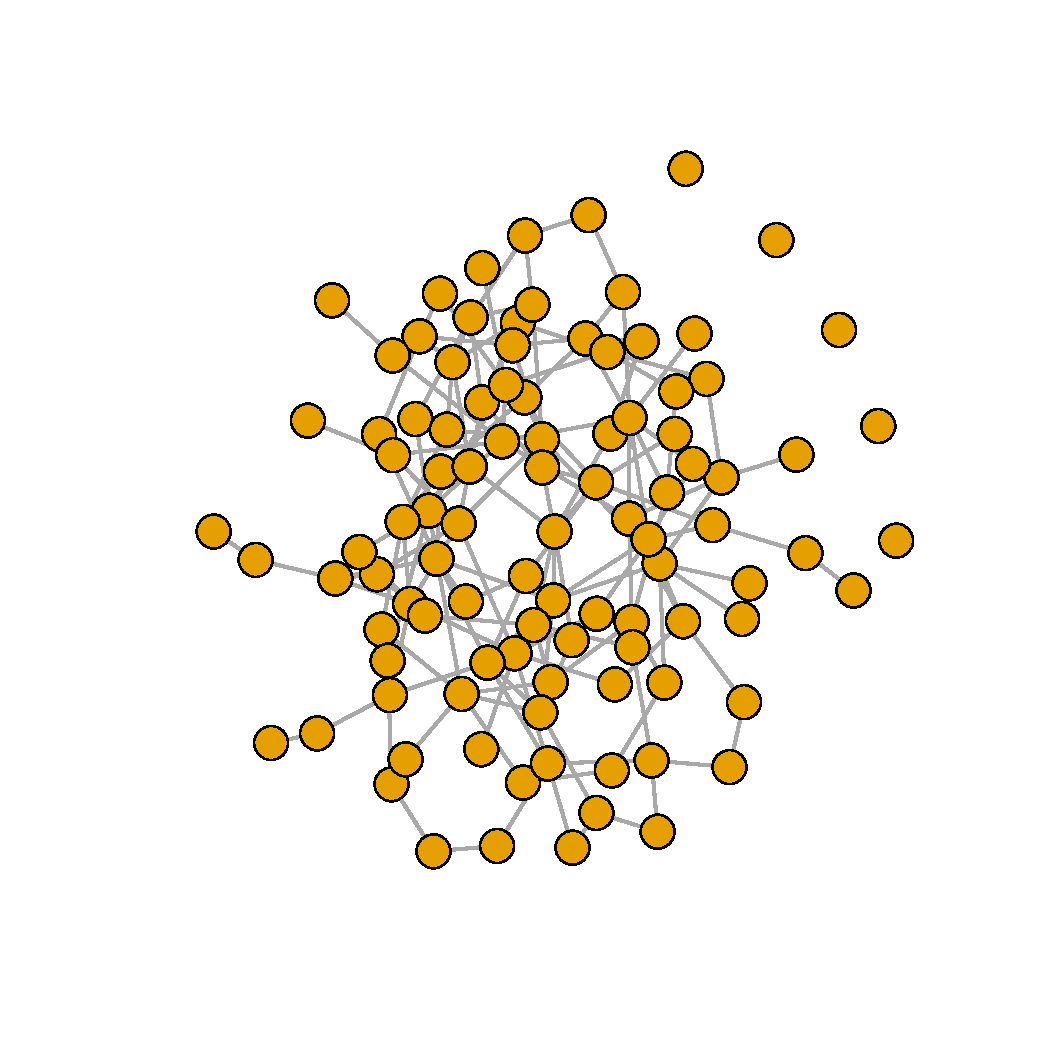
\includegraphics[scale=.3]{plots/ER.pdf} 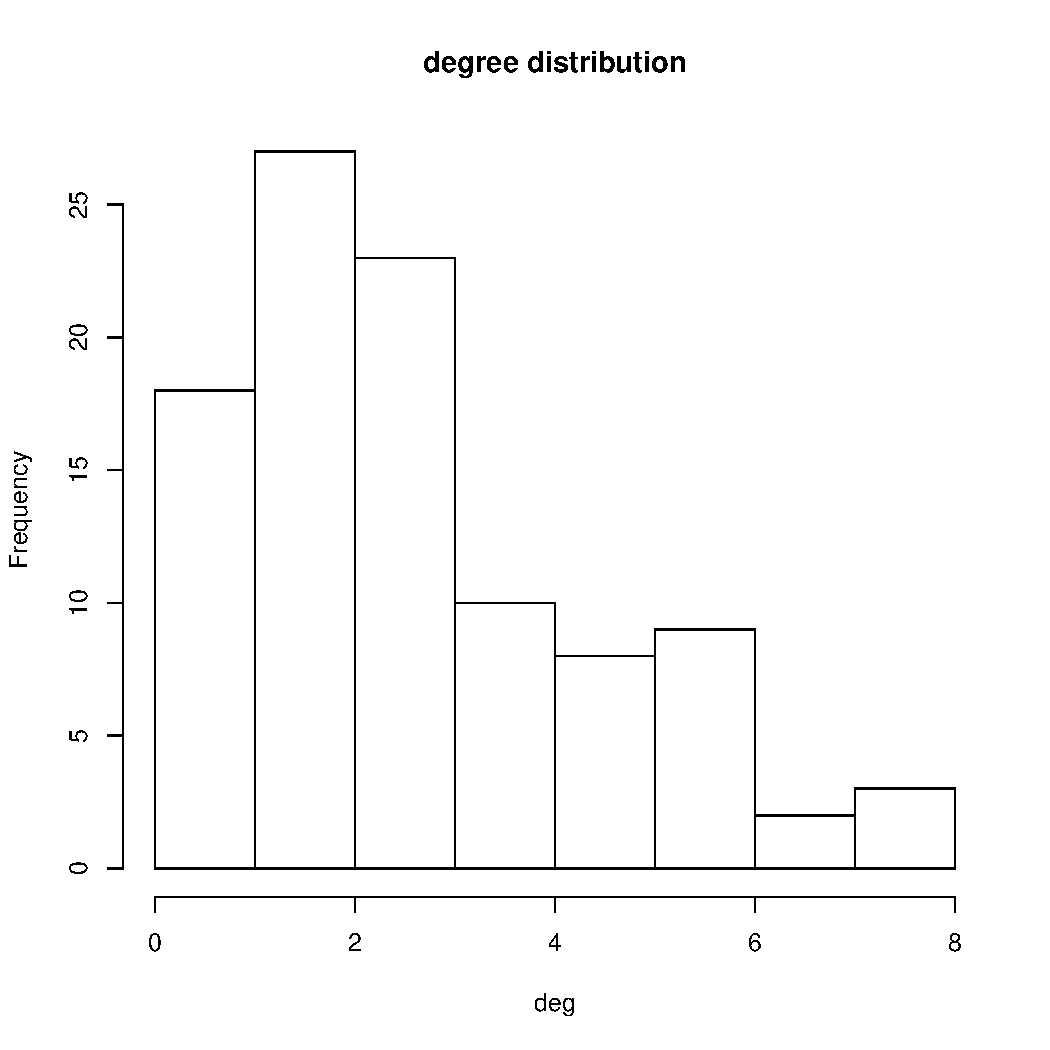
\includegraphics[scale=.3]{plots/degER.pdf}
\end{center}


\end{frame}


\begin{frame}
 \frametitle{Limitations of an ER graph to describe real networks}
 
 
 
\begin{itemize}
 \item Degree distribution too concentrated, no high degree nodes,
 \item all nodes are equivalent (no nestedness...),
 \item no modularity.

 \end{itemize}

\end{frame}






\section{Stochastic Block Model for classical networks}
%chilean web



\begin{frame}
  \frametitle{Stochastic Block Model}

  \begin{center}
    \begin{overlayarea}{\textwidth}{.5\textheight}
      \begin{columns}
        \begin{column}{.45\paperwidth}
        \begin{tikzpicture}
          %% UN GRAPH

          \tikzstyle{every edge}=[-,>=stealth',shorten >=1pt,auto,thin,draw]
          \tikzstyle{every state}=[draw=none,text=white,scale=0.65, font=\scriptsize, transform shape]
          \tikzstyle{every node}=[fill=yellow!40!orange]
          % premier cluster
          \node[state] (A1) at (0,0.5) {A1};
          \node[state] (A2) at (1,0.5) {A2};
          \node[state] (A3) at (.5,1.5) {A3};

          \path (A2) edge [bend left] node[fill=white,below=.1cm]
          {$\pi_{\textcolor{yellow!40!orange}{\bullet}\textcolor{yellow!40!orange}{\bullet}}$}
          (A1)
          (A1) edge [bend left] (A3)
          (A3) edge [bend left] (A2);

          \tikzstyle{every node}=[fill=blue!80!black]
          \foreach \angle/\text in {234/B1, 162/B2, 90/B3, 18/B4, -54/B5} {
            \node[fill=blue,state,xshift=5cm,yshift=3.5cm]     (\text)    at
            (\angle:1cm) {\text};
          }
          \path (B2) edge (B5)
          (B1) edge (B4);
          \foreach \from/\to in {1/2,2/3,4/5,5/1}{
            \path (B\from) edge [bend left] (B\to);
          }

          \path    (B3)    edge     [bend    left]    node[fill=white]
          {$\pi_{\textcolor{blue!80!black}{\bullet}\textcolor{blue!80!black}{\bullet}}$}  (B4) ;
          
          \tikzstyle{every node}=[fill=green!50!black]
          % troisieme cluster
          \node[state] (C1) at (3,-.5) {C1};
          \node[state] (C2) at (4,0) {C2};

          \path (C1) edge [bend right] node[fill=white,below=.25cm]
          {$\pi_{\textcolor{green!50!black}{\bullet}\textcolor{green!50!black}{\bullet}}$}
          (C2);

          % inter cluster
          \path (A3) edge [bend right]  (B2)
          (A3)    edge    [bend    left]    node[fill=white]
          {$\pi_{\textcolor{yellow!40!orange}{\bullet}\textcolor{blue!80!black}{\bullet}}$}
          (B3)
          (C2) edge [bend right] node[fill=white,right]
          {$\pi_{\textcolor{blue!80!black}{\bullet}\textcolor{green!50!black}{\bullet}}$}
          (B4)
          (A2) edge [bend right] node[fill=white]
          {$\pi_{\textcolor{yellow!40!orange}{\bullet}\textcolor{green!50!black}{\bullet}}$}
          (C1);
        \end{tikzpicture}
        \end{column}
        \begin{column}{.5\paperwidth}
          \begin{small}
            \begin{block}{Stochastic Block Model}
              Let $n$ nodes divided into
              \begin{itemize}
              \item
                $\mathcal{Q}=\{\textcolor{yellow!40!orange}{\bullet},\textcolor{blue!80!black}{\bullet},\textcolor{green!50!black}{\bullet}\}$
                classes
              \item  $\alpha_\bullet  =  \mathbb{P}(i  \in  \bullet)$,
                $\bullet\in\mathcal{Q},i=1,\dots,n$
              \item      $\pi_{\textcolor{yellow!40!orange}{\bullet}\textcolor{blue!80!black}{\bullet}}     =      \mathbb{P}(i
                \leftrightarrow j | i\in\textcolor{yellow!40!orange}{\bullet},j\in\textcolor{blue!80!black}{\bullet})$
              \end{itemize}
            \end{block}
          \end{small}
        \end{column}
      \end{columns}
    \end{overlayarea}
  \end{center}
  
%\begin{eqnarray*}
%&(Z_i) &  \ \sim^{\text{iid}} \mathcal{M}(1,\alpha) \ \text{et} \  Z_{i} \in \{1,...,Q\}, \\ 
% &(X_{ij})&| \ \{Z_{i},Z_{j}\} \sim^{\text{ind}} \mathcal{B}(\pi_{Z_{i}Z_{j}}).\\
%\end{eqnarray*}

% Proposition Julien
\begin{align*}
Z_i = \mathbf{1}_{\{i \in \bullet\}}  \ & \sim^{\text{iid}} \mathcal{M}(1,\alpha), \quad \forall\bullet \in \mathcal{Q}, \\ 
X_{ij} \ | \ \{i\in\textcolor{yellow!40!orange}{\bullet},j\in\textcolor{blue!80!black}{\bullet}\}
& \sim^{\text{ind}} \mathcal{B}(\pi_{\textcolor{yellow!40!orange}{\bullet}\textcolor{blue!80!black}{\bullet}})\\
\end{align*}

\end{frame}




\begin{frame}
\frametitle{Some remarkable structure generated with SBM : networks with hubs}

\centering
\begin{tabular}{ccc}
 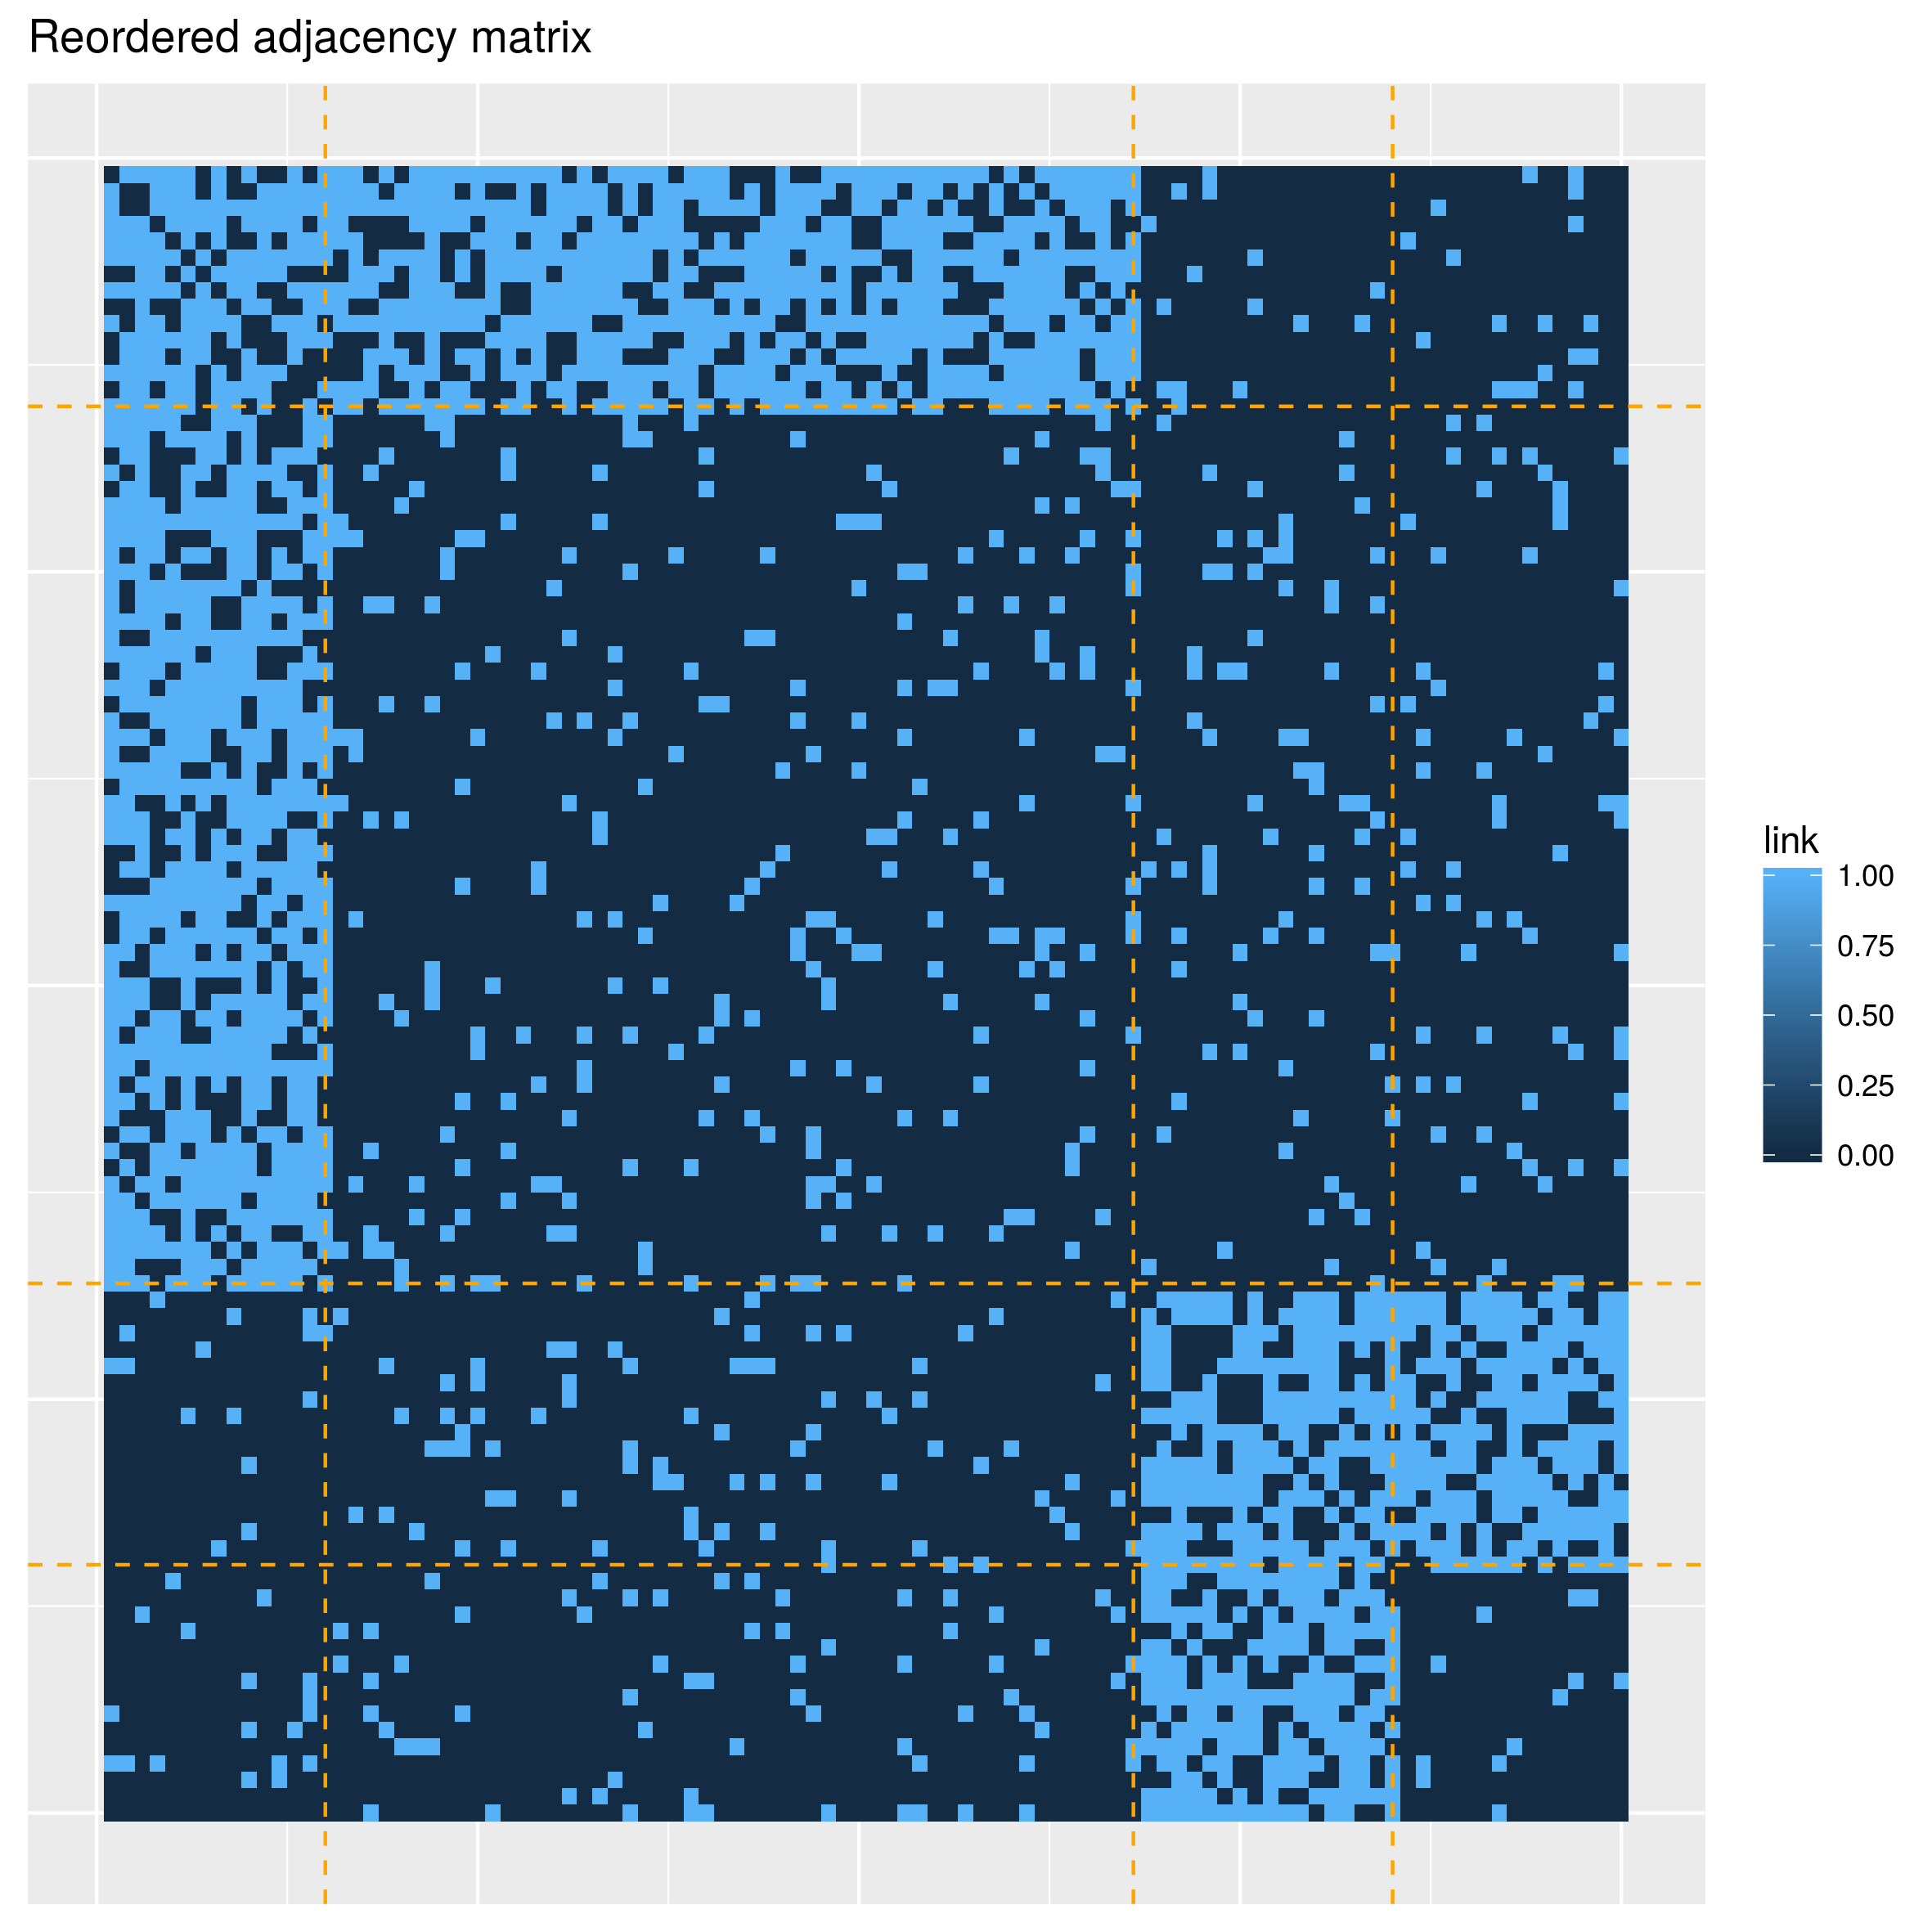
\includegraphics[scale=.2]{plots/sbm/Etoile_reordered_adja_with_groups.png}&
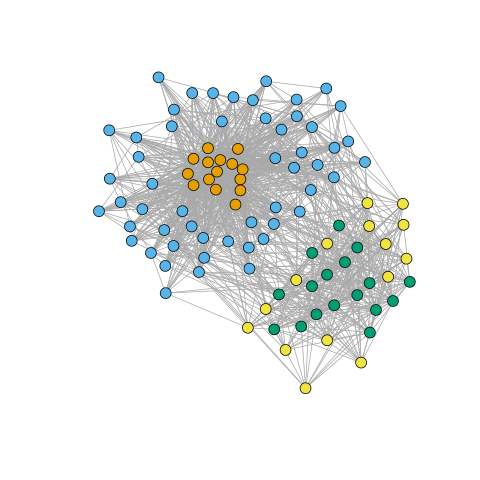
\includegraphics[scale=.2]{plots/sbm/Etoile_graphe_with_colors.png}&
   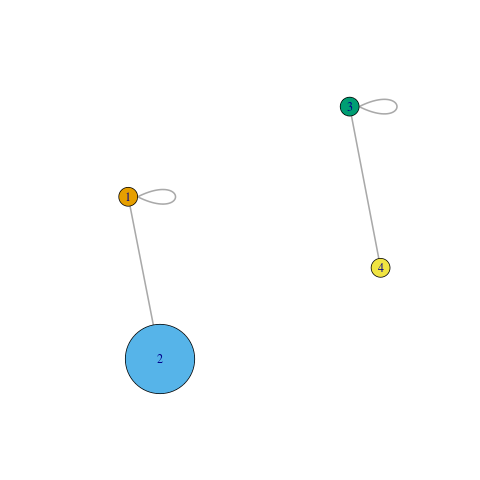
\includegraphics[scale=.2]{plots/sbm/Etoile_graphe_resume.png}
 \end{tabular}

\begin{tabular}{cc}
    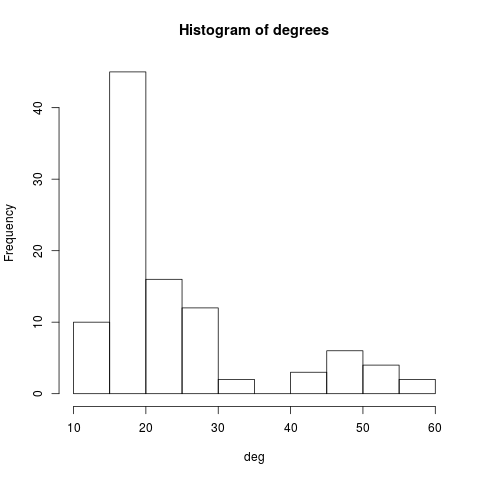
\includegraphics[scale=.2]{plots/sbm/Etoile_histogram_degree.png}&
   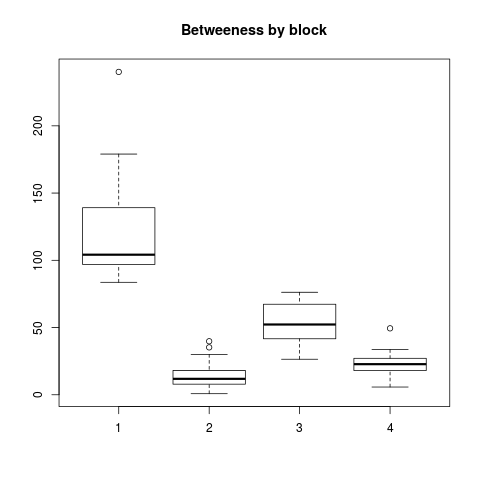
\includegraphics[scale=.2]{plots/sbm/Etoile_betweeness.png}
 \end{tabular}

\end{frame}



\begin{frame}
\frametitle{Some remarkable structure generated with SBM : community network}

\centering
\begin{tabular}{cc}
 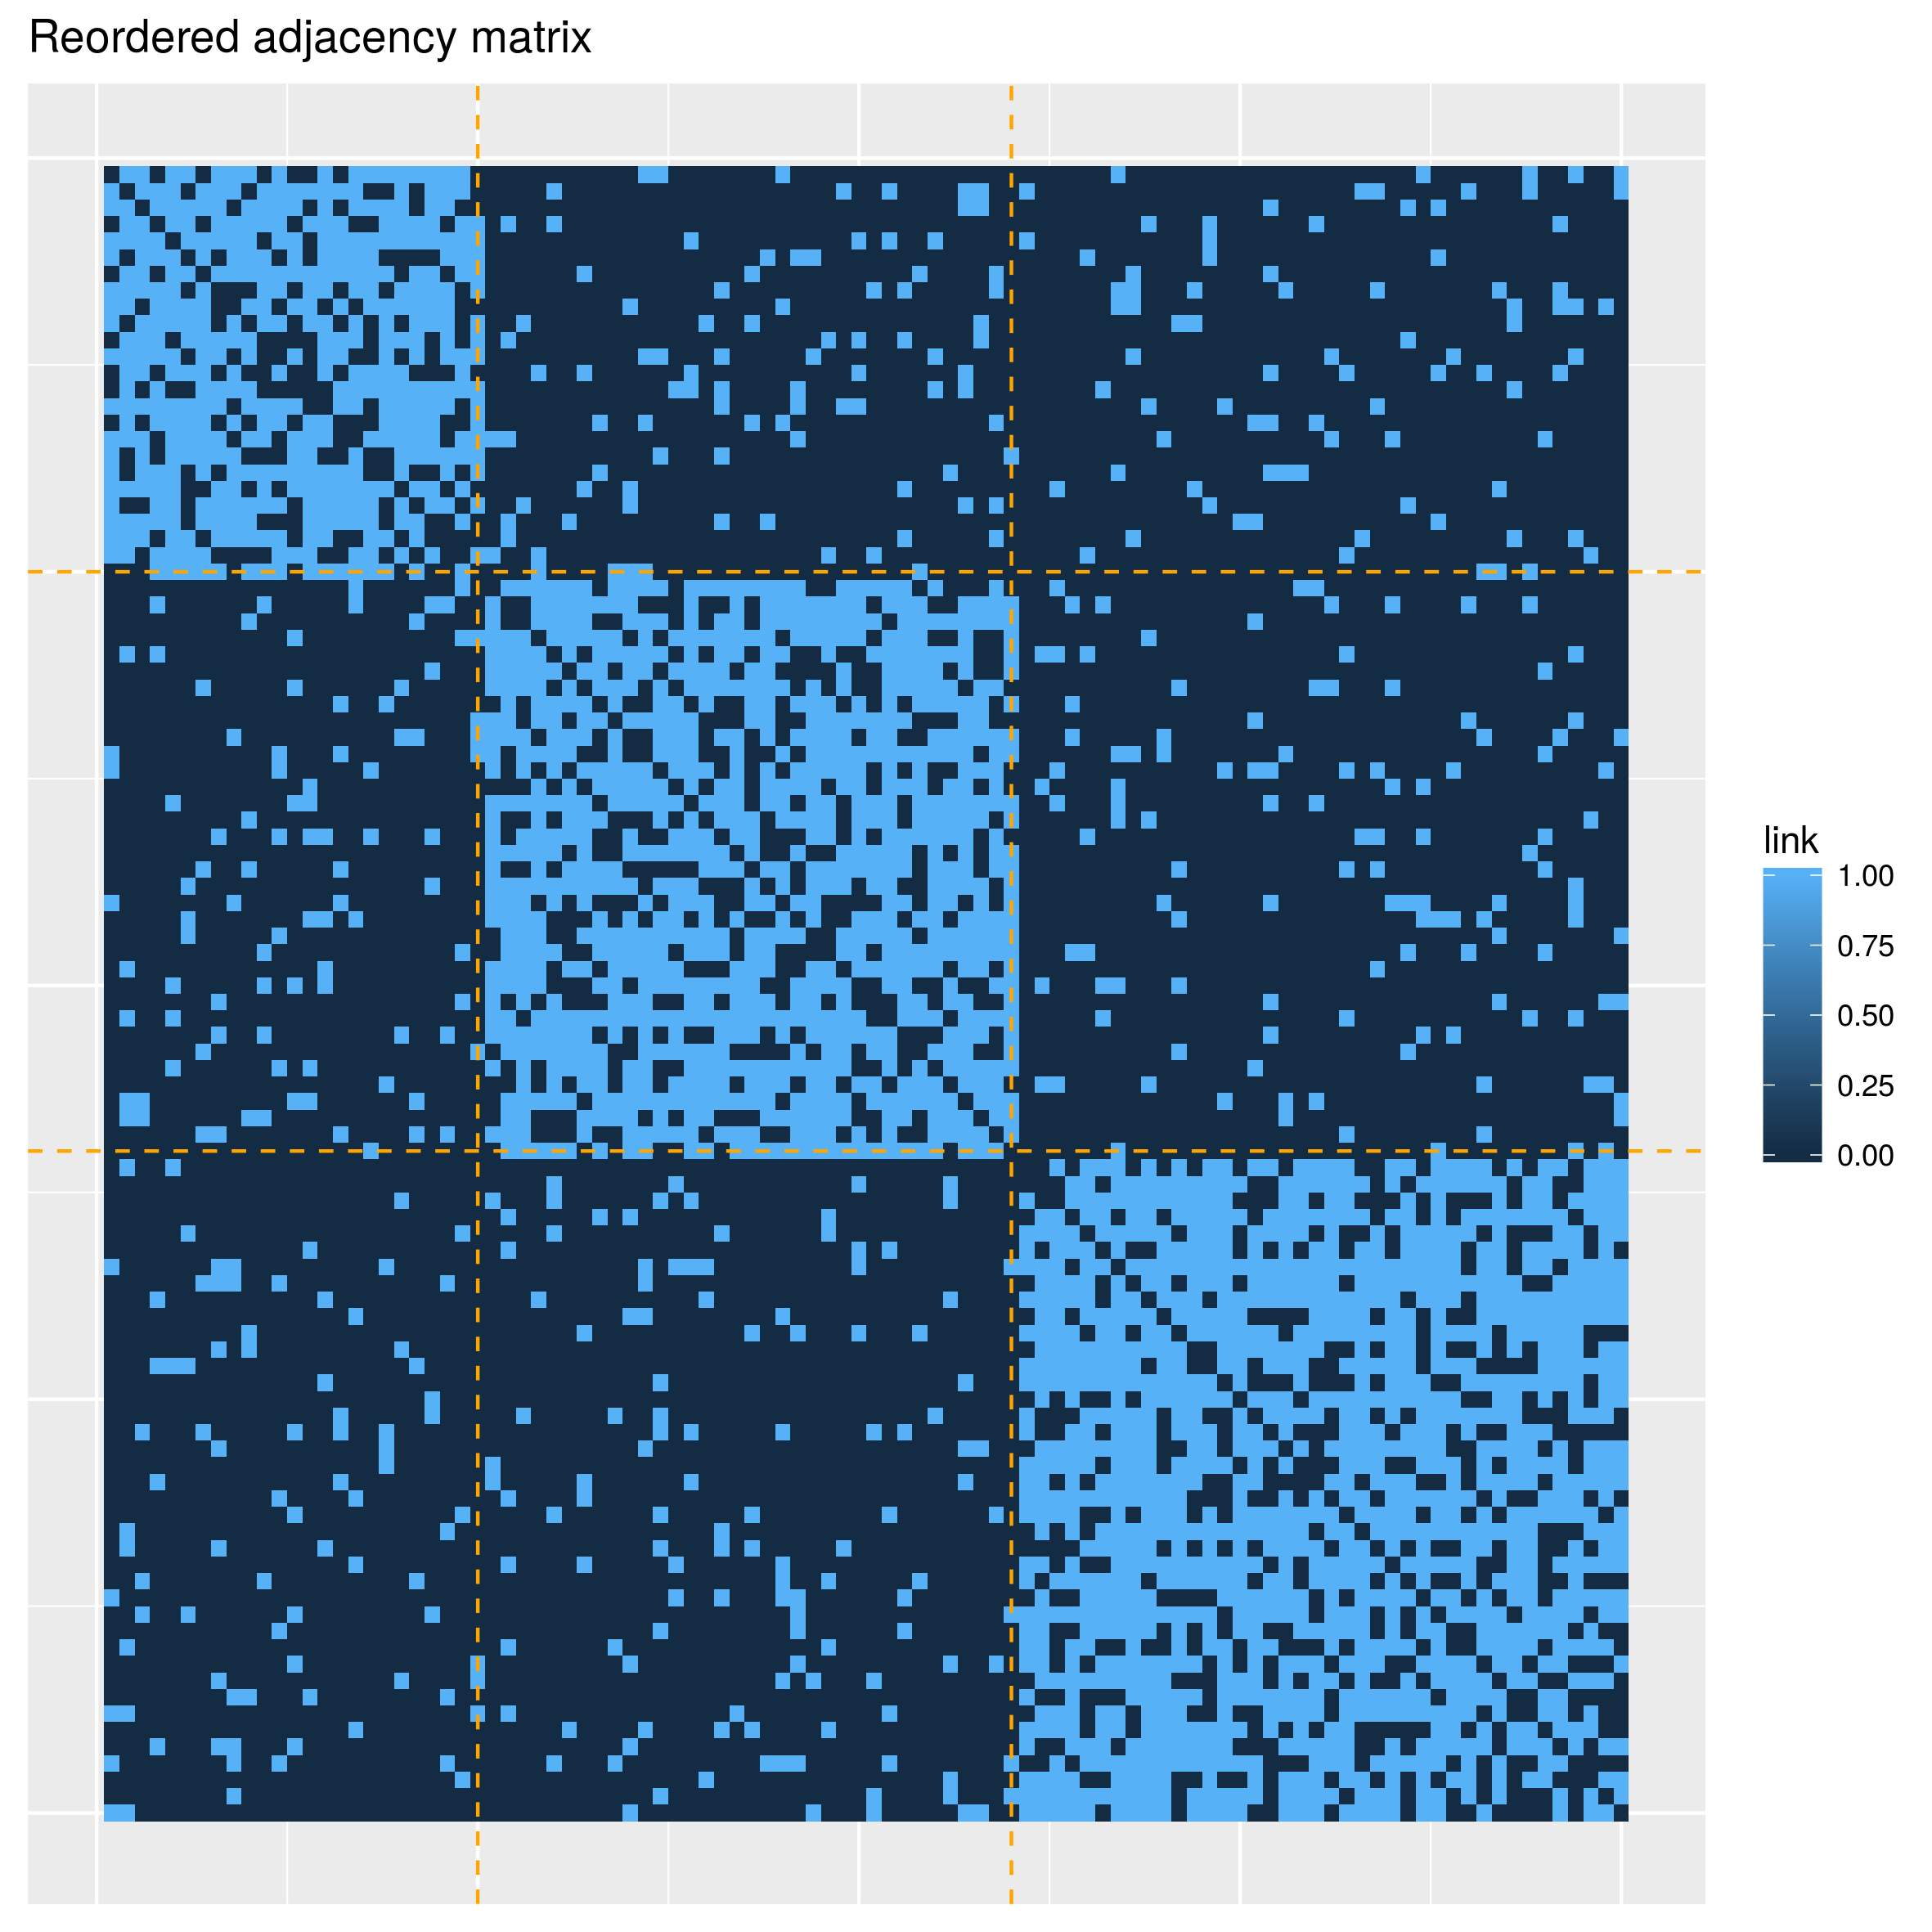
\includegraphics[scale=.2]{plots/sbm/Affiliation_reordered_adja_with_groups.png}&
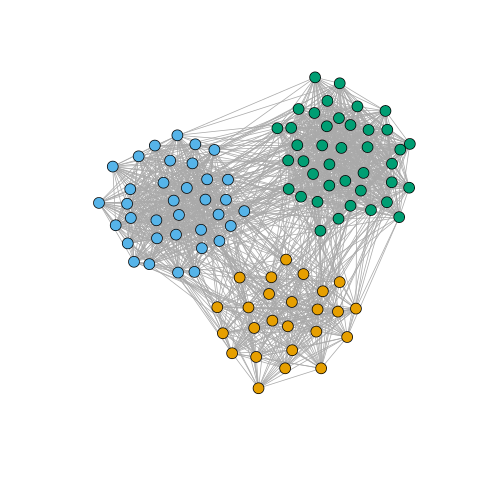
\includegraphics[scale=.2]{plots/sbm/Affiliation_graphe_with_colors.png} 
 \end{tabular}

\begin{tabular}{cc}
   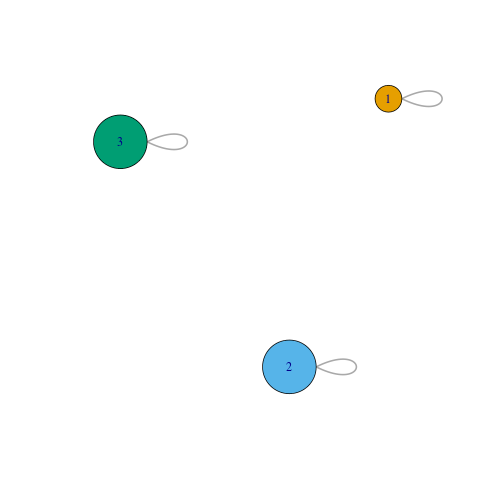
\includegraphics[scale=.2]{plots/sbm/Affiliation_graphe_resume.png}
    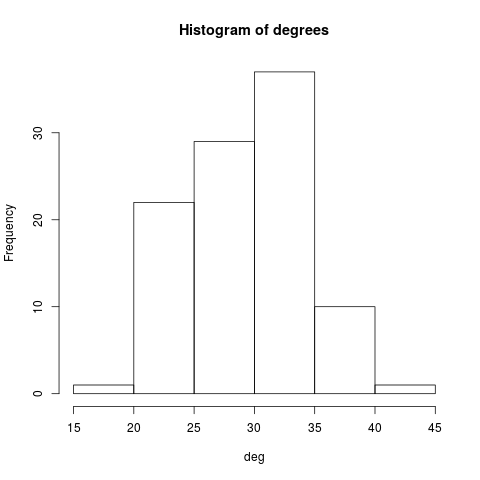
\includegraphics[scale=.2]{plots/sbm/Affiliation_histogram_degree.png}&
 \end{tabular}

\end{frame}


\begin{frame}
\frametitle{Some remarkable structure generated with SBM : nestedness}

\centering
\begin{tabular}{cc}
 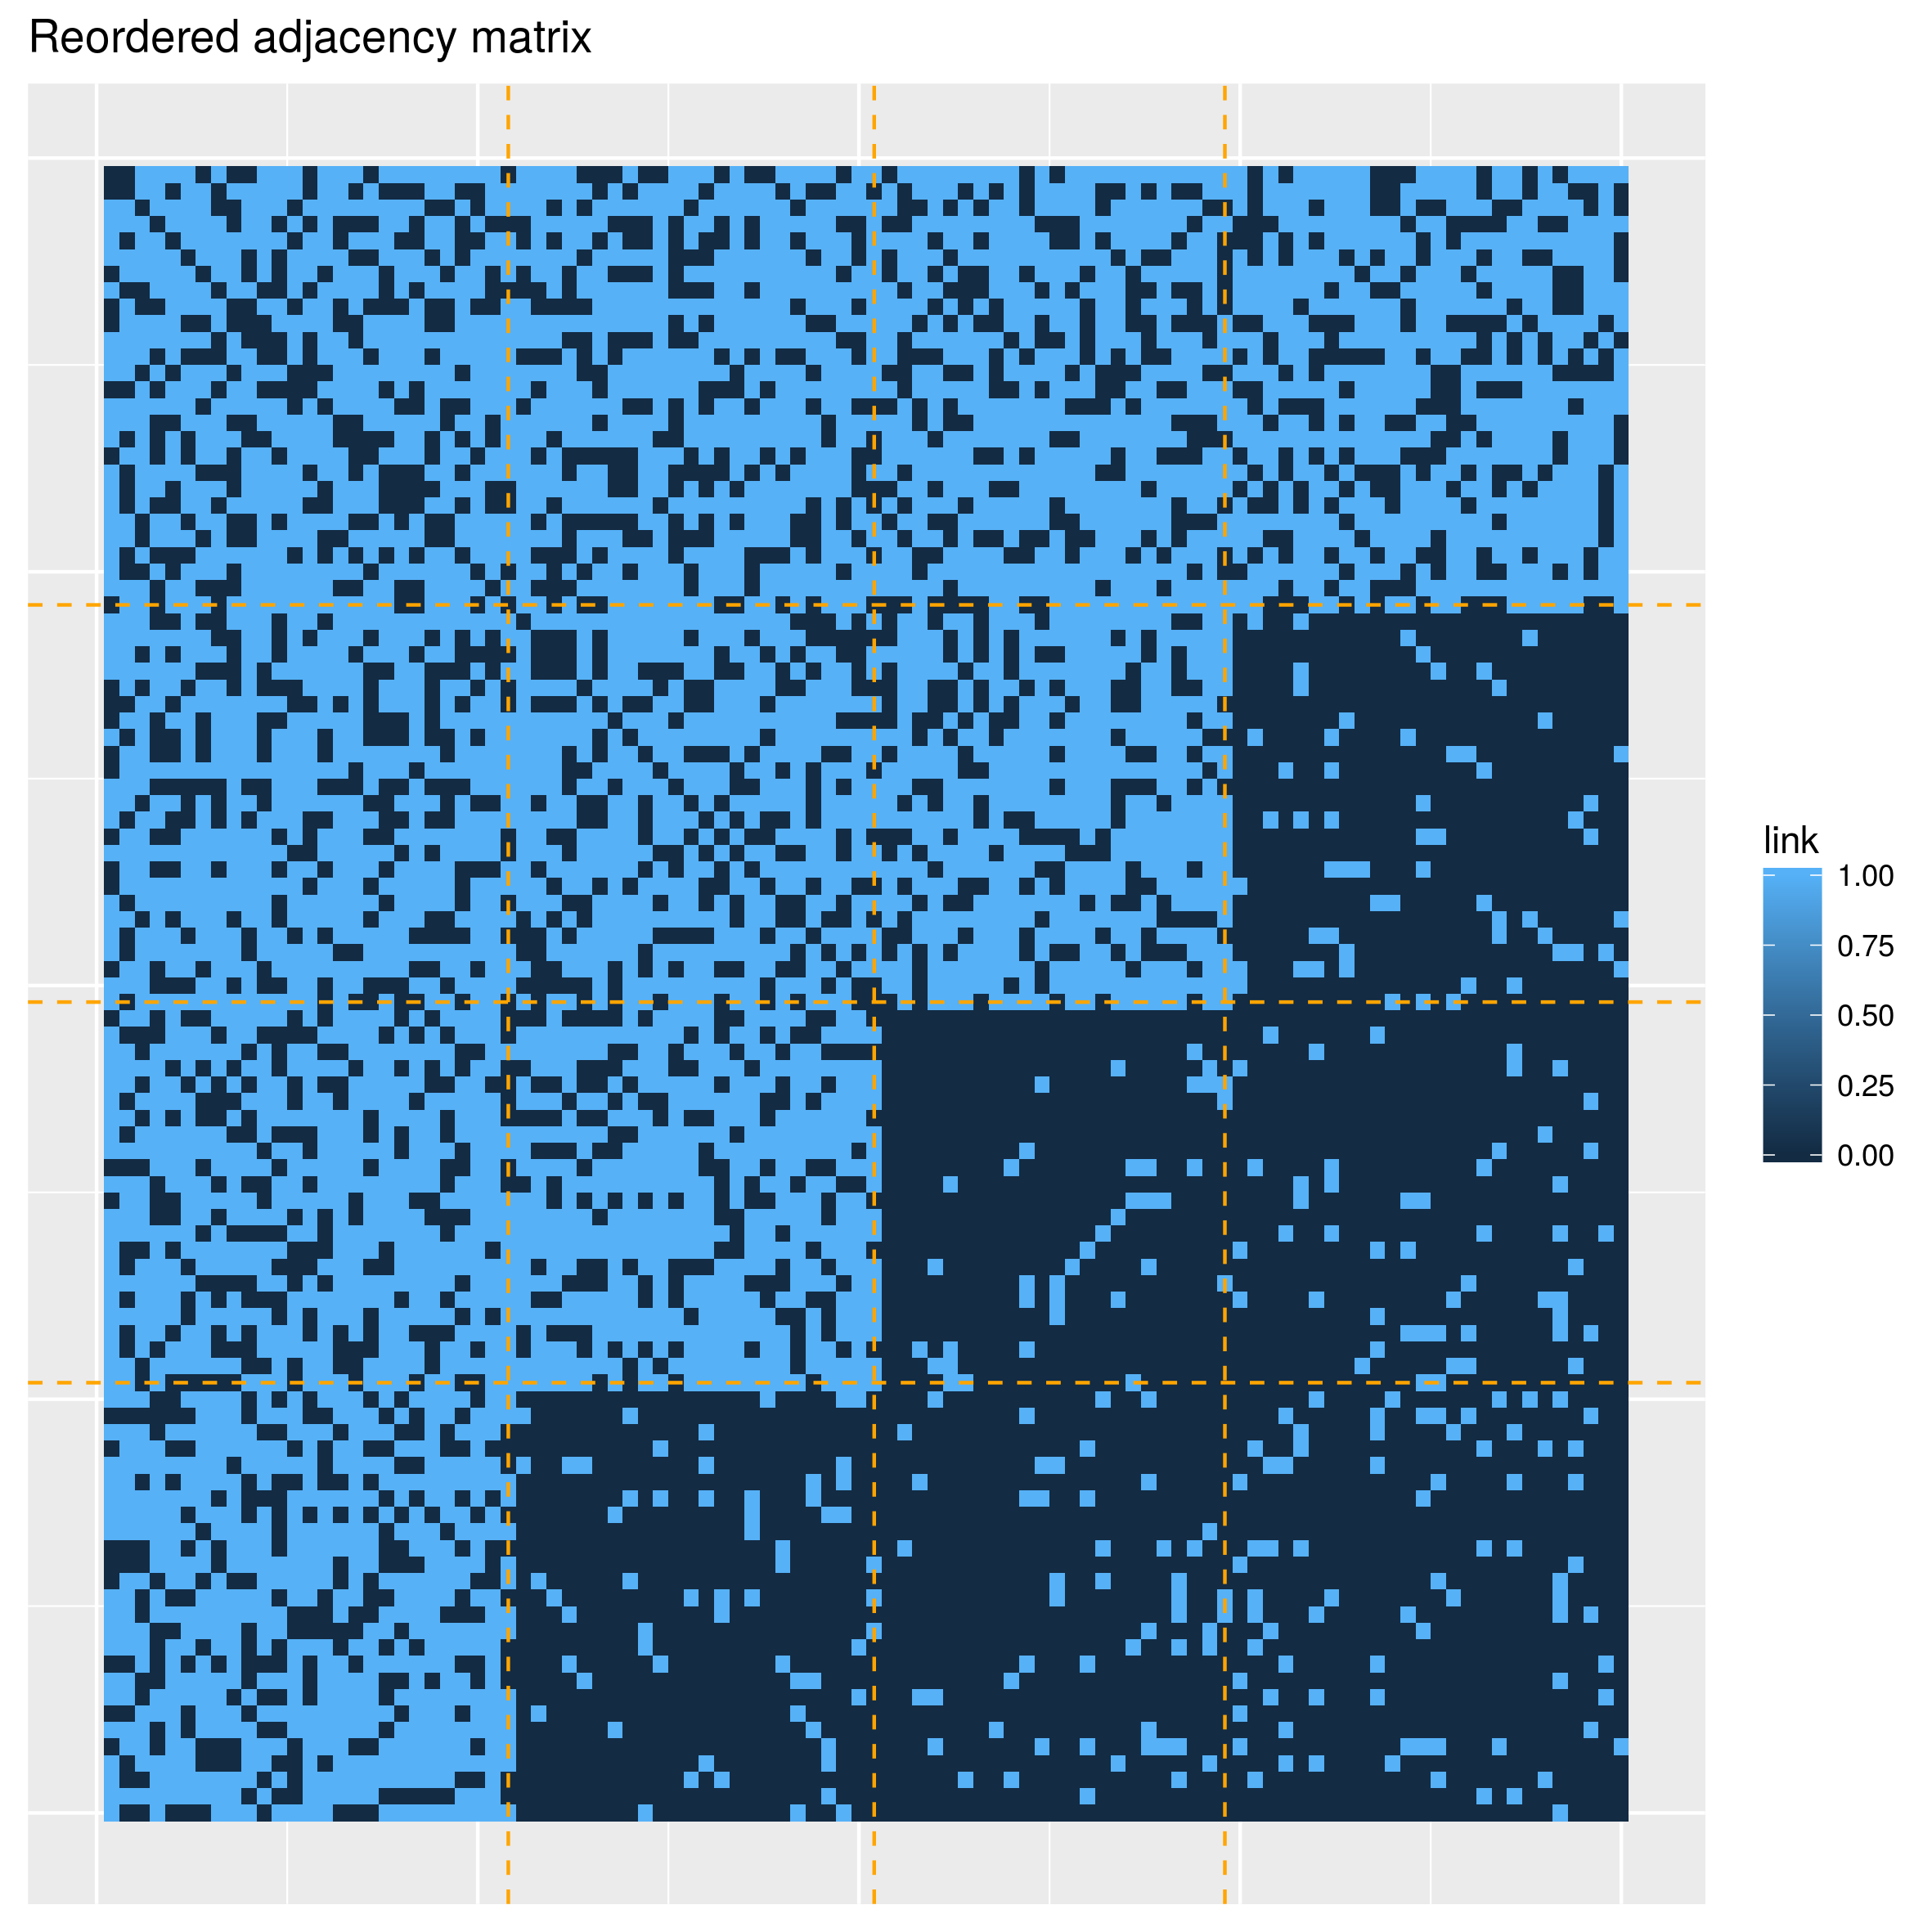
\includegraphics[scale=.2]{plots/sbm/Nested_reordered_adja_with_groups.png}&
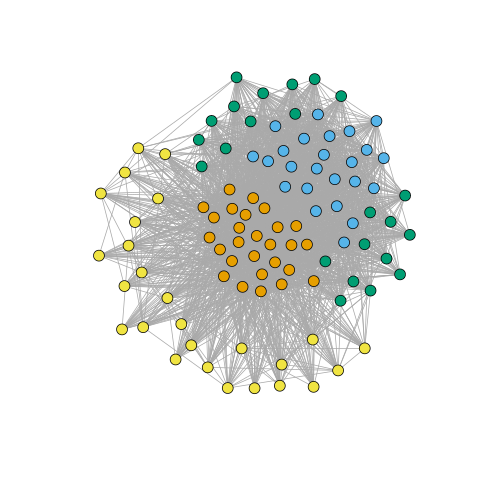
\includegraphics[scale=.2]{plots/sbm/Nested_graphe_with_colors.png} 
 \end{tabular}

\begin{tabular}{cc}
   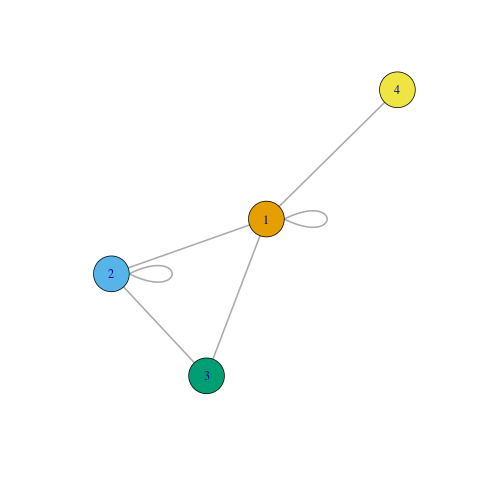
\includegraphics[scale=.2]{plots/sbm/Nested_graphe_resume.png}
    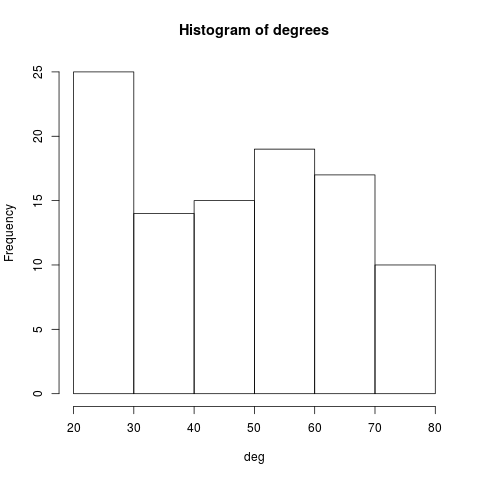
\includegraphics[scale=.2]{plots/sbm/Nested_histogram_degree.png}&
 \end{tabular}

\end{frame}




\begin{frame}
  \frametitle{Statistical inference}
 
    \begin{center}
  \begin{overlayarea}{\textwidth}{.5\textheight}
      \begin{columns}
        \begin{column}{.45\paperwidth}
        \begin{tikzpicture}
          %% UN GRAPH

          \tikzstyle{every edge}=[-,>=stealth',shorten >=1pt,auto,thin,draw]
          \tikzstyle{every state}=[draw=none,text=white,scale=0.65, font=\scriptsize, transform shape]
          \tikzstyle{every node}=[fill=lightgray]
          % premier cluster
          \node[state] (A1) at (0,0.5) {N1};
          \node[state] (A2) at (1,0.5) {N2};
          \node[state] (A3) at (.5,1.5) {N3};

          \path (A2) edge [bend left] node[fill=white,below=.1cm]
          {}
          (A1)
          (A1) edge [bend left] (A3)
          (A3) edge [bend left] (A2);

          \tikzstyle{every node}=[fill=blue!80!black]
          \foreach \angle/\text in {234/N1, 162/N2, 90/N3, 18/N4, -54/N5} {
            \node[fill=lightgray,state,xshift=5cm,yshift=3.5cm]     (\text)    at
            (\angle:1cm) {\text};
          }
          \path (B2) edge (B5)
          (B1) edge (B4);
          \foreach \from/\to in {1/2,2/3,4/5,5/1}{
            \path (B\from) edge [bend left] (B\to);
          }

          \path    (B3)    edge     [bend    left]    node[fill=white]
          {}  (B4) ;
          
          \tikzstyle{every node}=[fill=lightgray]
          % troisime cluster
          \node[state] (C1) at (3,-.5) {N1};
          \node[state] (C2) at (4,0) {N2};

          \path (C1) edge [bend right] (C2);

          % inter cluster
          \path (A3) edge [bend right]  (B2)
          (A3)    edge    [bend    left]    node[fill=white]
          {}
          (B3)
          (C2) edge [bend right] node[fill=white,right]
          {}
          (B4)
          (A2) edge [bend right] node[fill=white]
          {}
          (C1);
        \end{tikzpicture}
        \end{column}
        \begin{column}{.5\paperwidth}
          \begin{small}
            \begin{block}{Stochastic Block Model}
              Let $n$ nodes divided into
              \begin{itemize}
              \item
                $\mathcal{Q}=\{\textcolor{yellow!40!orange}{\bullet},\textcolor{blue!80!black}{\bullet},\textcolor{green!50!black}{\bullet}\}$,
                $\text{card}(\mathcal{Q})$ known
              \item  $\alpha_\bullet  =  ?$,
              \item      $\pi_{\textcolor{yellow!40!orange}{\bullet}\textcolor{blue!80!black}{\bullet}}     =      ?$
              \end{itemize}
            \end{block}
          \end{small}
        \end{column}
      \end{columns}
    \end{overlayarea}
    \end{center}
    \medskip

    
    \textcolor{blue}{Nowicki, \& Snijders (2001), Daudin et al. (2008)}
    
    \bigskip
    
\textcolor{blue}{R package: blockmodels.}
%     
%     \begin{thebibliography}{99}
%       \begin{scriptsize}
%       \bibitem[NS]{NS} Nowicki, Snijders, JASA, 2001 \newblock Estimation and prediction for
%         stochastic   blockstructures.
%         \textcolor{black}{} 
%       \bibitem[DRP]{DRP}   Daudin,  Picard,   Robin,  Statistics   and
%         Computing, 2008 \newblock A mixture model for random graphs. 
%       \end{scriptsize}
%   \end{thebibliography}

\end{frame}



\begin{frame}\frametitle{Statistical inference} 

From.... 

\centering
\begin{tabular}{cc}
 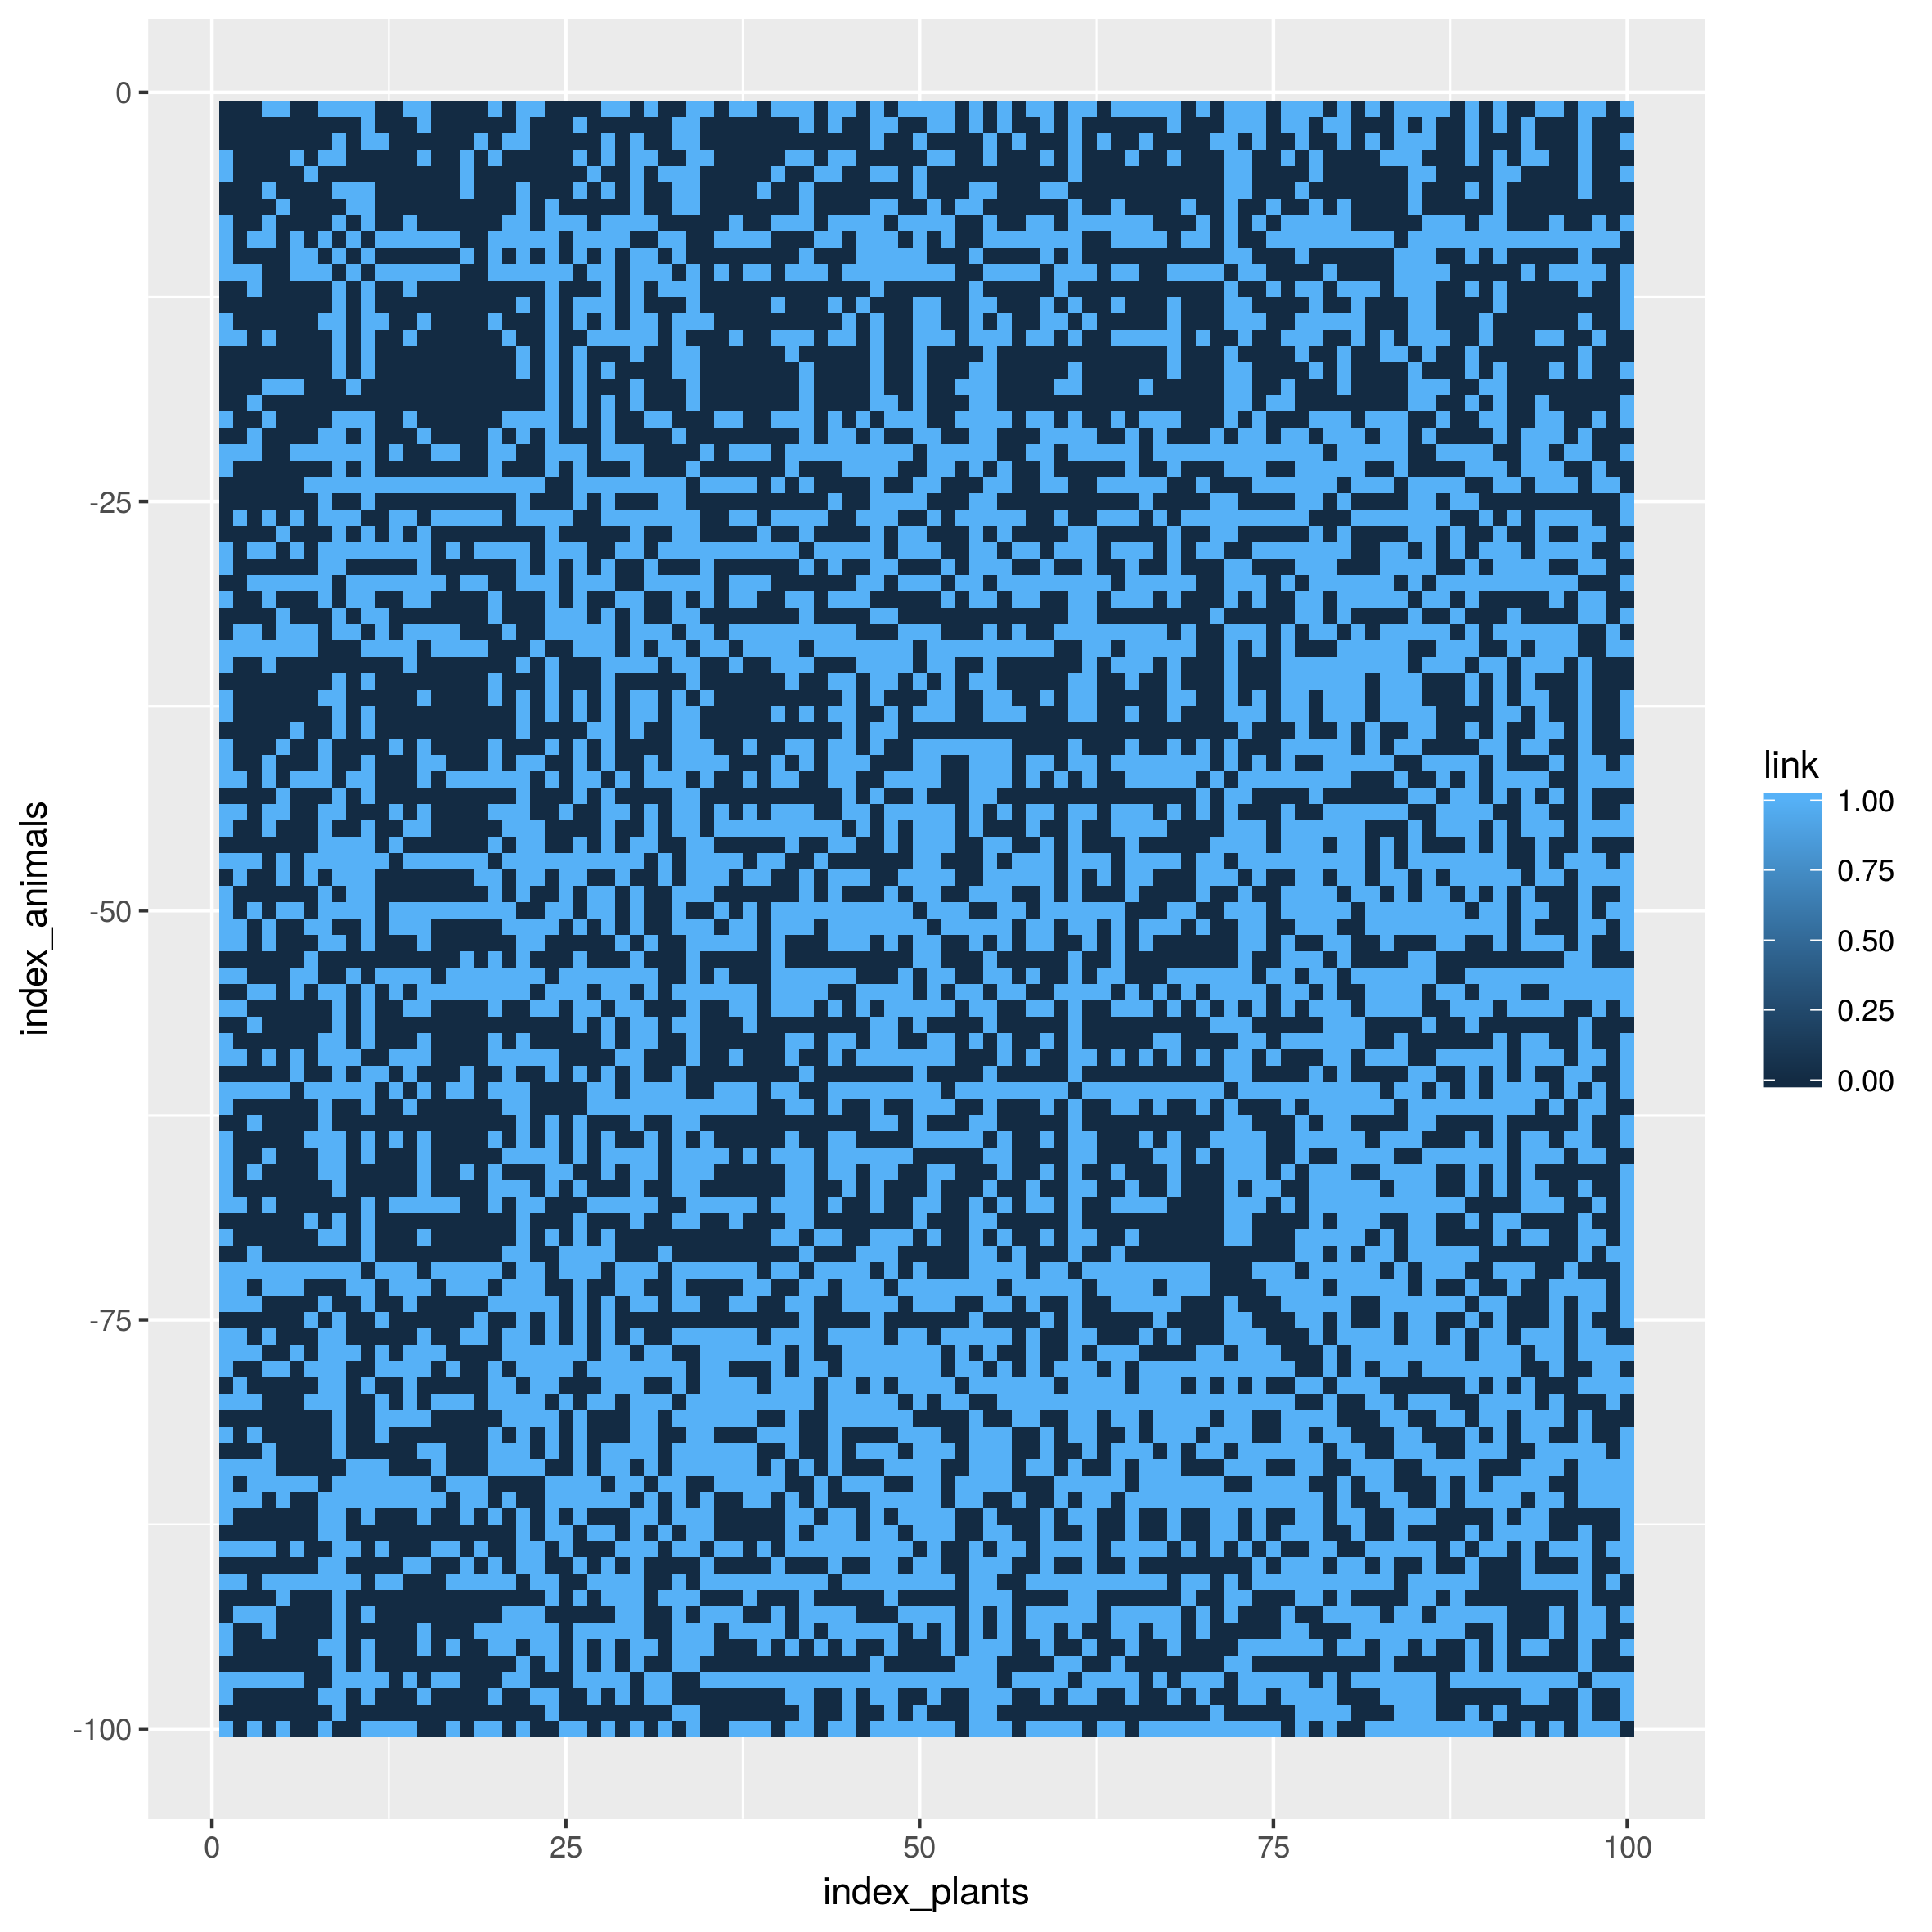
\includegraphics[scale=.2]{plots/sbm/Nested_adja.png}&
 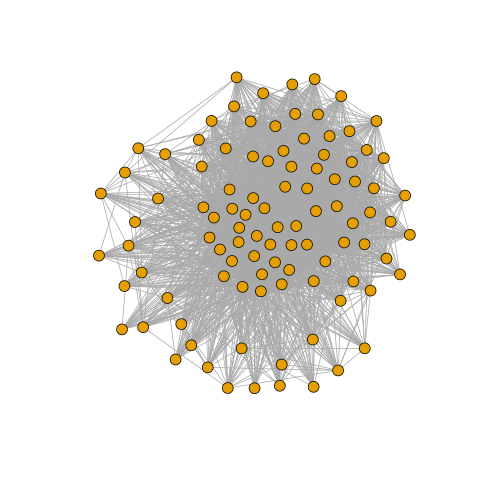
\includegraphics[scale=.2]{plots/sbm/Nested_graphe_without_colors.png}
\end{tabular}
\end{frame}

\begin{frame}\frametitle{Statistical inference} 

... to 

\centering
\begin{tabular}{cc}
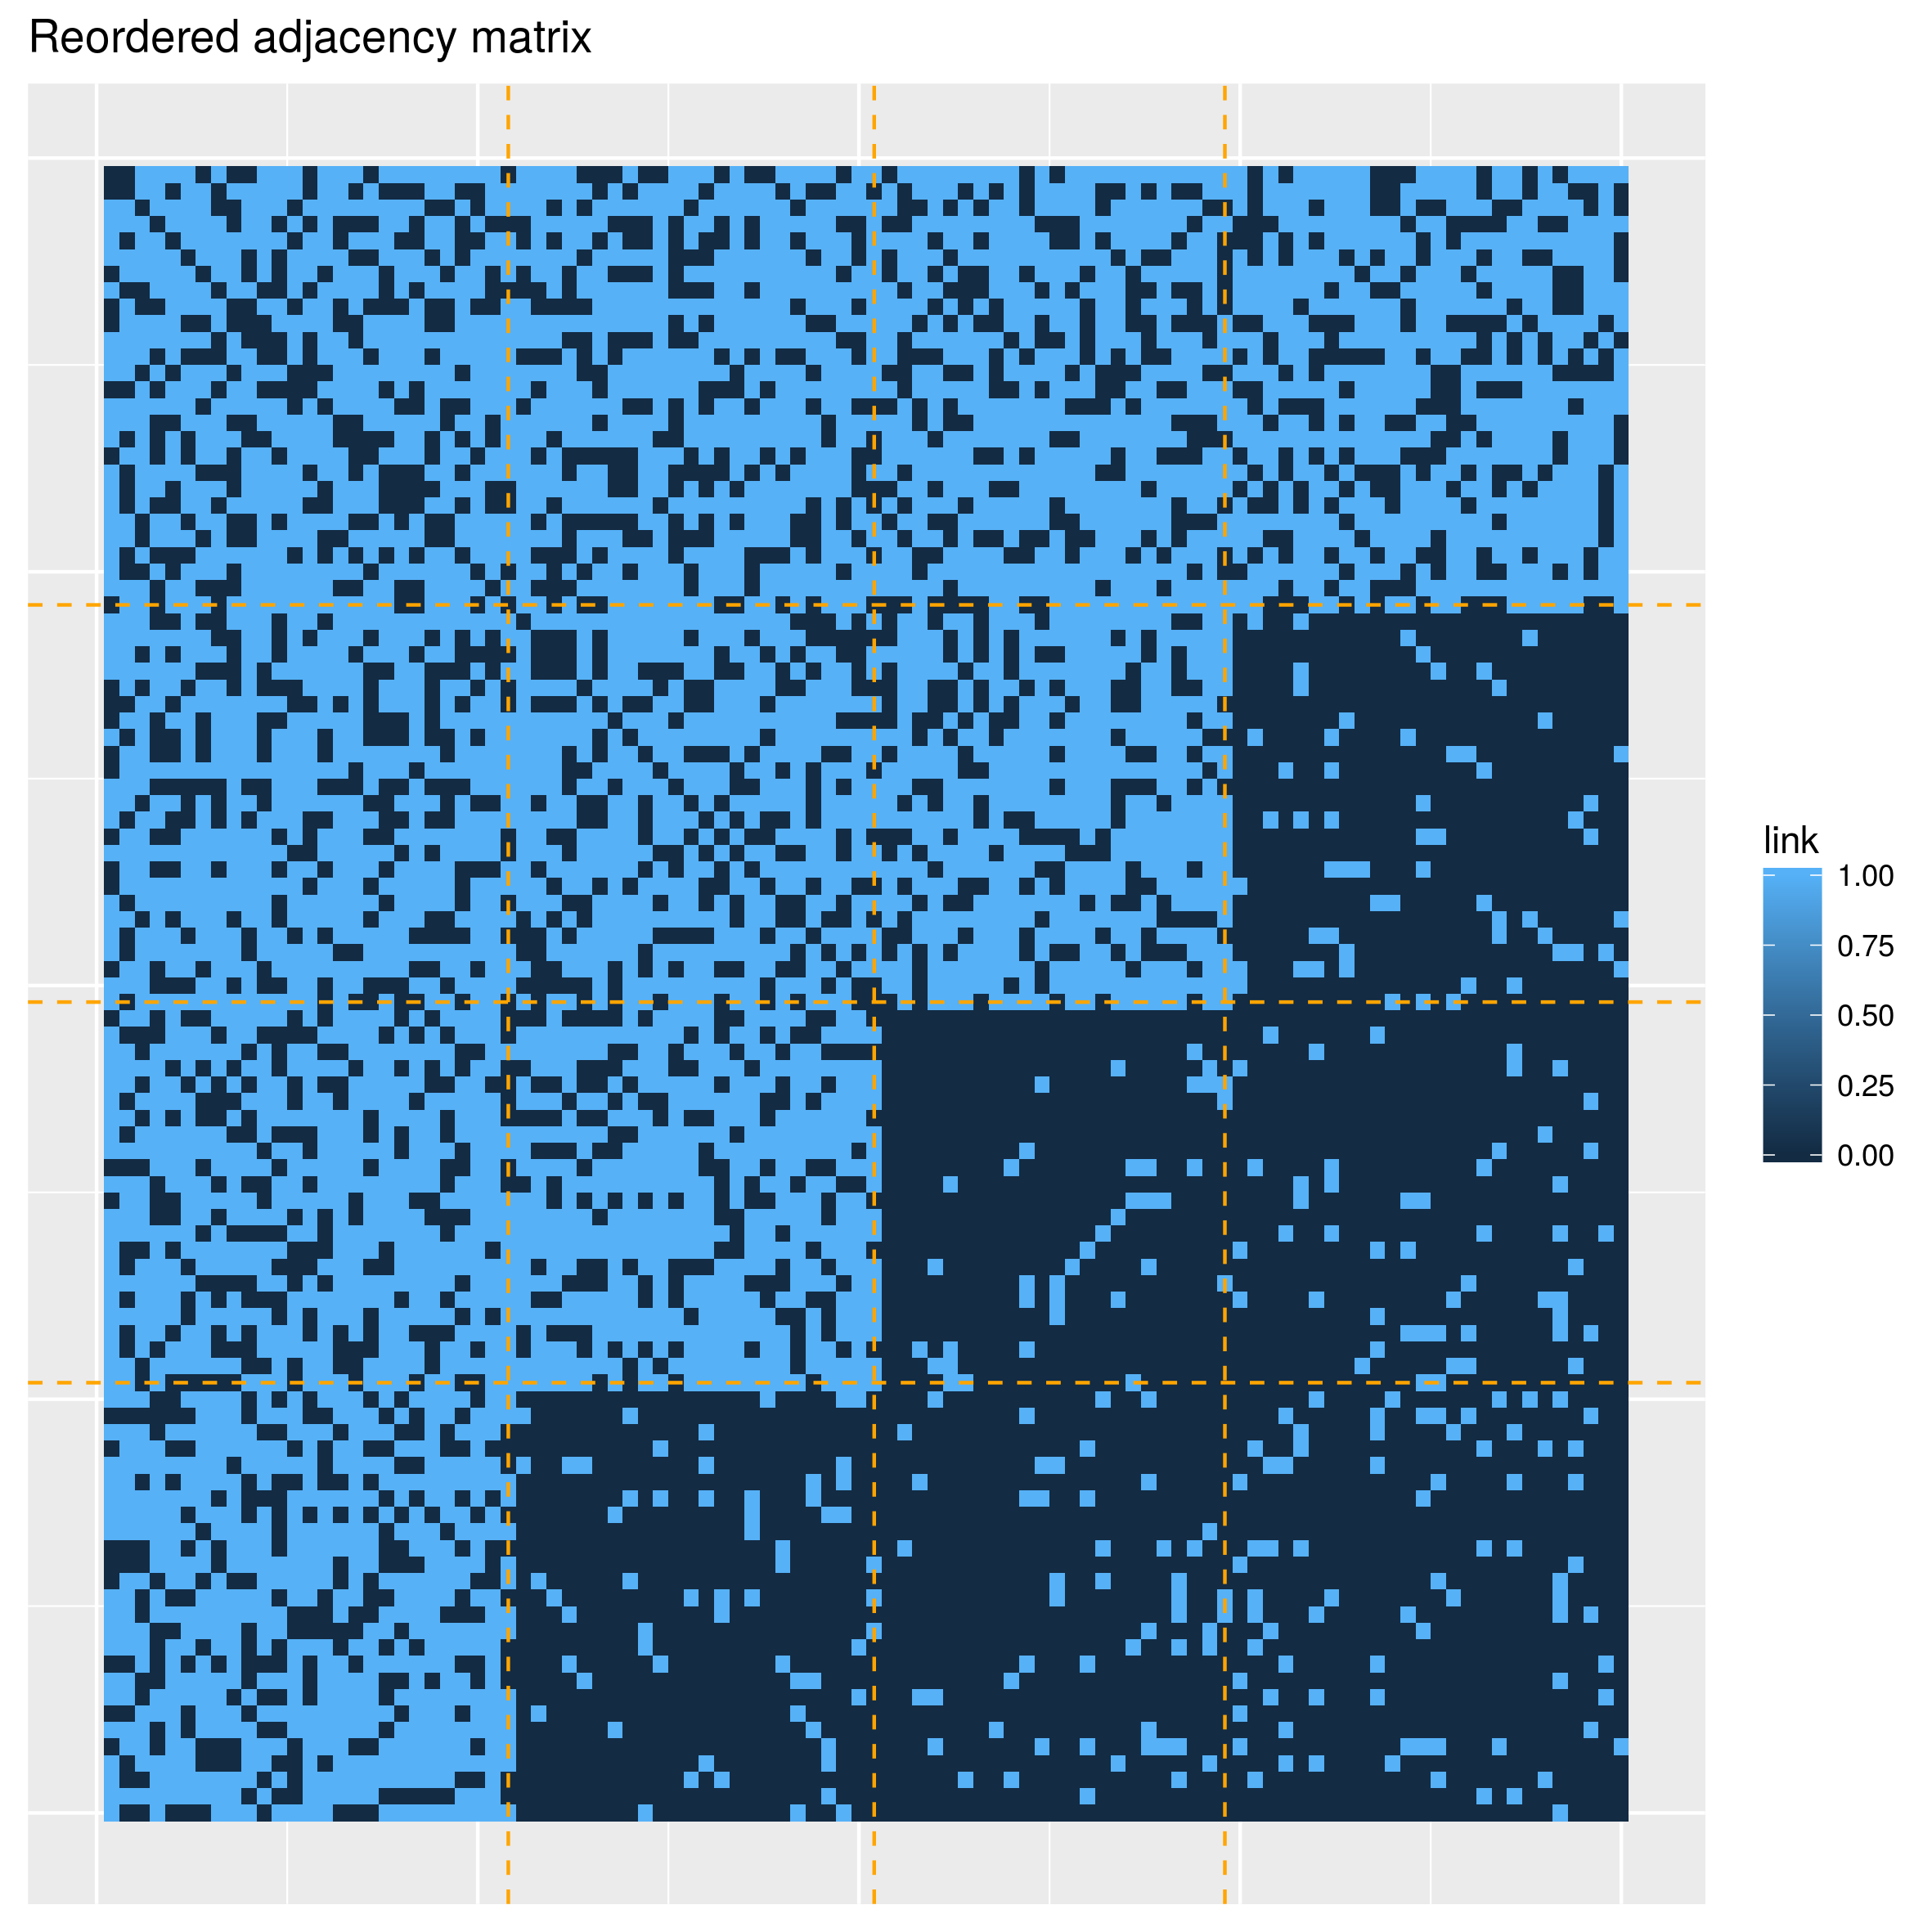
\includegraphics[scale=.2]{plots/sbm/Nested_reordered_adja_with_groups.png}
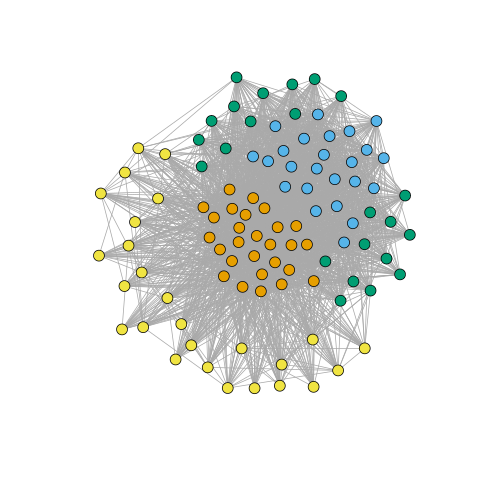
\includegraphics[scale=.2]{plots/sbm/Nested_graphe_with_colors.png}
\end{tabular}

\begin{block}{Statistician job}
\begin{itemize}
\item Find the clusters
\item Find the number of clusters
\item Practical implementation
\item Theoretical results
\end{itemize}
\end{block}

\end{frame}


\begin{frame}
 \frametitle{Application to the Chilean food web}
 
 \begin{center}
  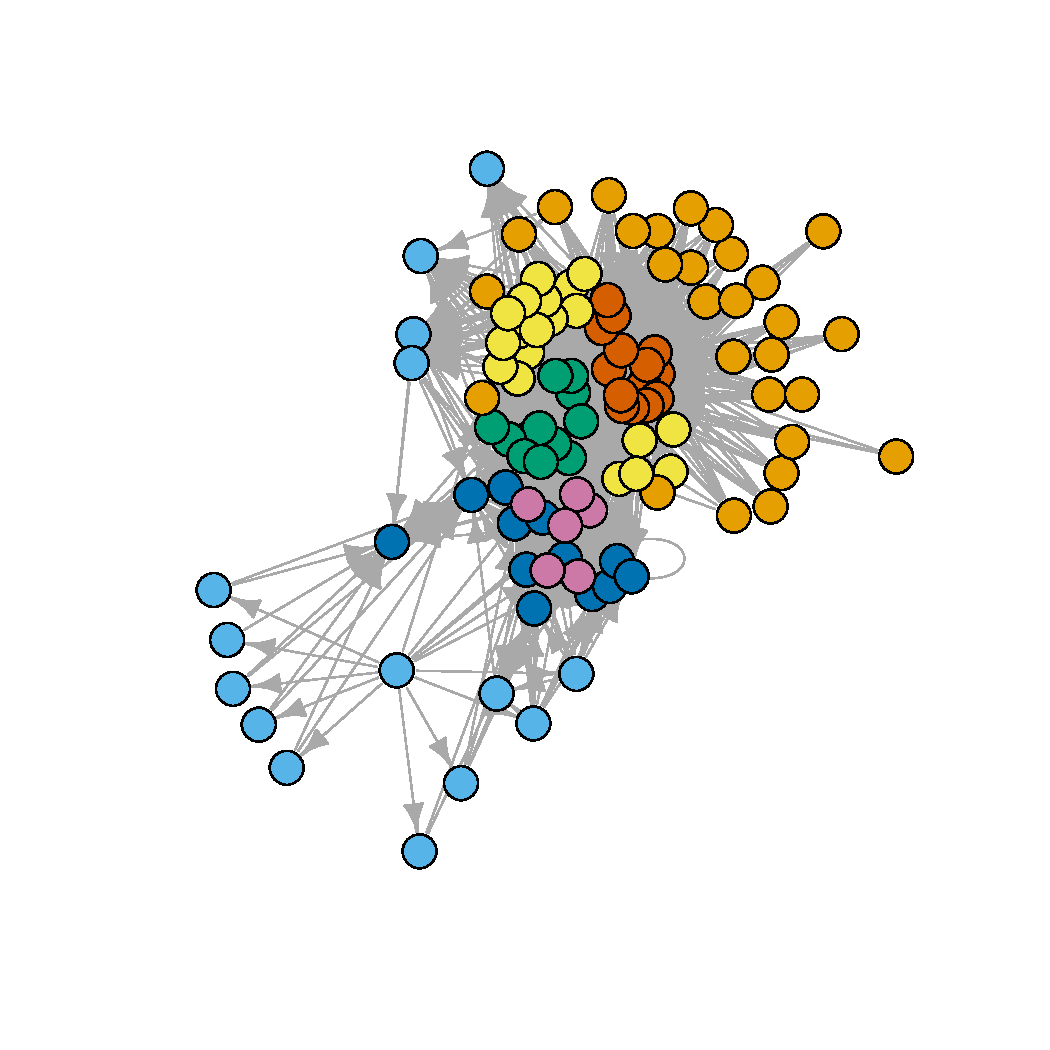
\includegraphics[scale=.3]{plots/chilean_sbm.pdf}
 \end{center}

 \begin{itemize}
 \item $7$ groups/blocks/clusters found,
 \item \begin{tabular}{rrrrrrr}
  \hline
  1 & 2 & 3 & 4 & 5 & 6 & 7 \\ 
  \hline
  28 &  15 &  12 &  19 &  12 &  14 &   6 \\ 
   \hline
\end{tabular}
\end{itemize}


\end{frame}


\begin{frame}
 \frametitle{Application to the Chilean food web}
 
 \begin{center}
  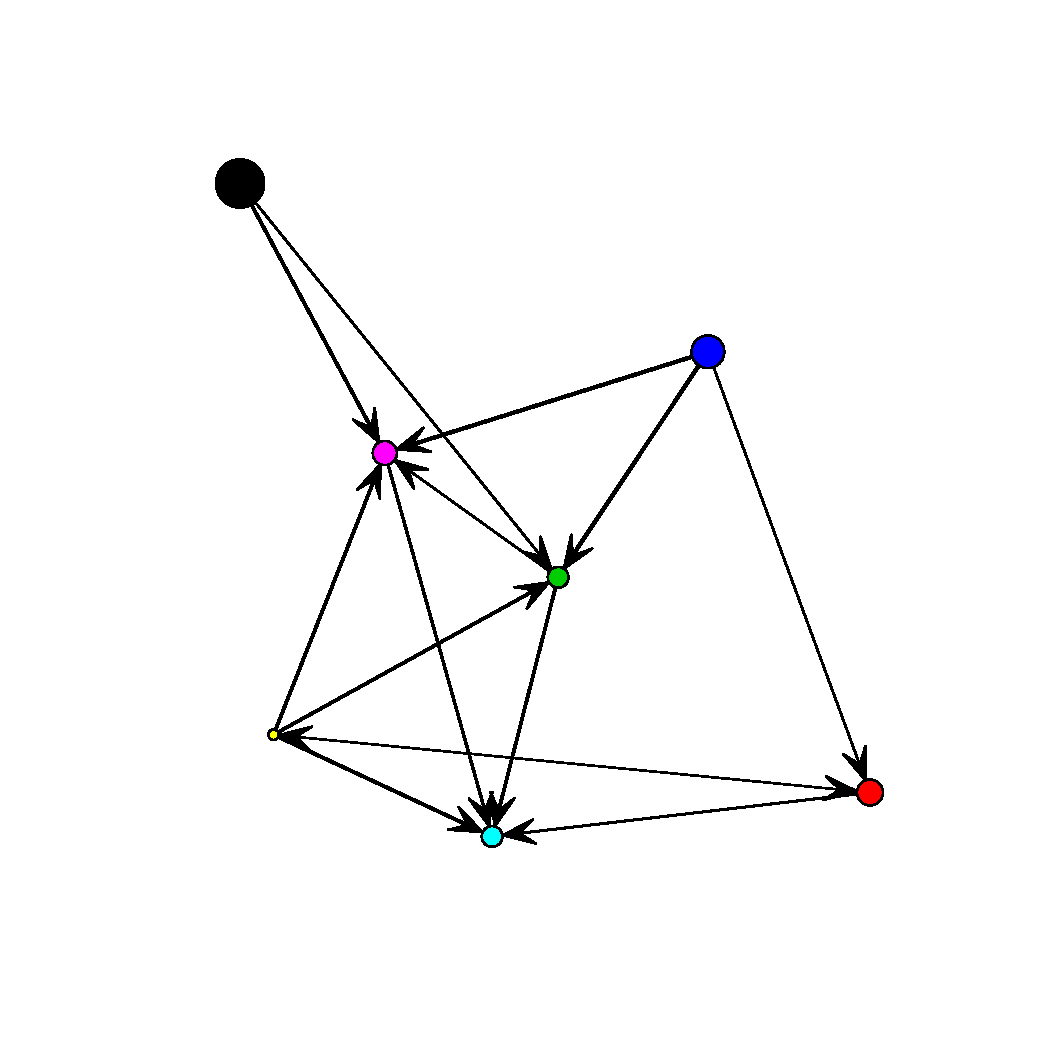
\includegraphics[scale=.3]{plots/chilean_sbm_sum.pdf}
 \end{center}

 
 Another example for food web in \textcolor{blue}{Allesina \& Pascual (2009)}.
\end{frame}





\section{Latent Block Model for bipartite networks}
%reseau interaction qcq

\begin{frame}
\frametitle{Latent Block Model}

 \begin{center}
    \begin{overlayarea}{\textwidth}{.5\textheight}
      \begin{columns}
        \begin{column}{.45\paperwidth}
        \centering
        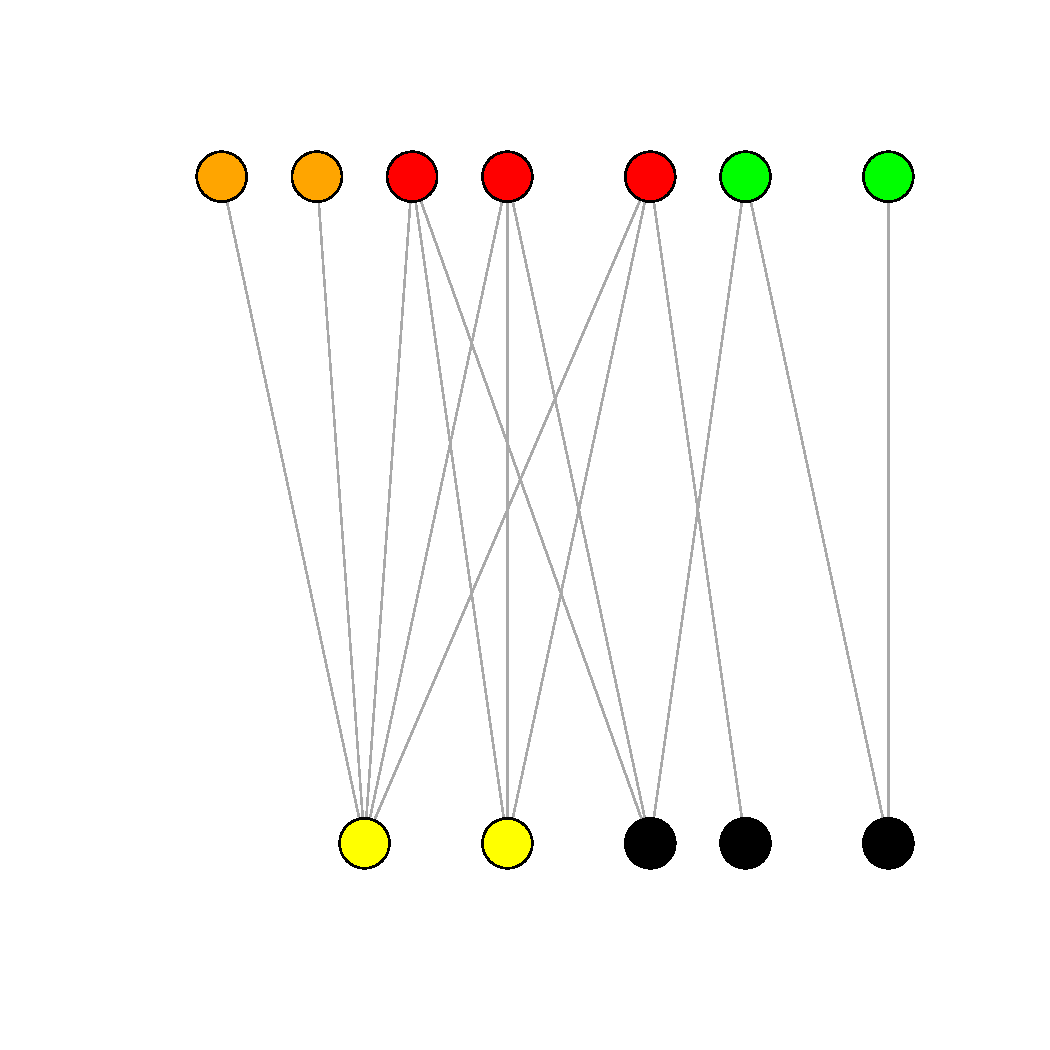
\includegraphics[scale=.3]{plots/LBM_exemple.pdf}
        \end{column}
        \begin{column}{.5\paperwidth}
          \begin{small}
            \begin{block}{Latent Block Model}
              \begin{itemize}
              \item
                $n$ row nodes $\mathcal{Q}_1=\{\textcolor{red}{\bullet},\textcolor{orange}{\bullet},\textcolor{green}{\bullet}\}$
                classes
              \item  $\alpha_\bullet  =  \mathbb{P}(i  \in  \bullet)$,
                $\bullet\in\mathcal{Q}_1,i=1,\dots,n$
              \item $m$ column nodes $\mathcal{Q}_2=\{\textcolor{yellow}{\bullet},\textcolor{black}{\bullet}\}$
                classes
               \item  $\beta_\bullet  =  \mathbb{P}(j  \in  \bullet)$,
                $\bullet\in\mathcal{Q}_2,j=1,\dots,m$
              \item      $\pi_{\textcolor{red}{\bullet}\textcolor{yellow}{\bullet}}     =      \mathbb{P}(i
                \leftrightarrow j | i\in\textcolor{red}{\bullet},j\in\textcolor{yellow}{\bullet})$
              \end{itemize}
            \end{block}
          \end{small}
        \end{column}
      \end{columns}
    \end{overlayarea}
  \end{center}
  
%\begin{eqnarray*}
%&(Z_i) &  \ \sim^{\text{iid}} \mathcal{M}(1,\alpha) \ \text{et} \  Z_{i} \in \{1,...,Q\}, \\ 
% &(X_{ij})&| \ \{Z_{i},Z_{j}\} \sim^{\text{ind}} \mathcal{B}(\pi_{Z_{i}Z_{j}}).\\
%\end{eqnarray*}

% Proposition Julien
\begin{align*}
Z_i = \mathbf{1}_{\{i \in \bullet\}}  \ & \sim^{\text{iid}} \mathcal{M}(1,\alpha), \quad \forall\bullet \in \mathcal{Q}_1, \\ 
W_j=\mathbf{1}_{\{j \in \bullet\}}  \ & \sim^{\text{iid}} \mathcal{M}(1,\beta), \quad \forall\bullet \in \mathcal{Q}_2, \\
X_{ij} \ | \ \{i\in\textcolor{red}{\bullet},j\in\textcolor{yellow}{\bullet}\}
& \sim^{\text{ind}} \mathcal{B}(\pi_{\textcolor{red}{\bullet}\textcolor{yellow}{\bullet}})\\
\end{align*}


\textcolor{blue}{Govaert \& Nadif (2008)} and 
\textcolor{blue}{R package: blockmodels} as well.

\end{frame}


\begin{frame}\frametitle{Incidence matrix point of view}

\centering
\begin{tabular}{cc}
 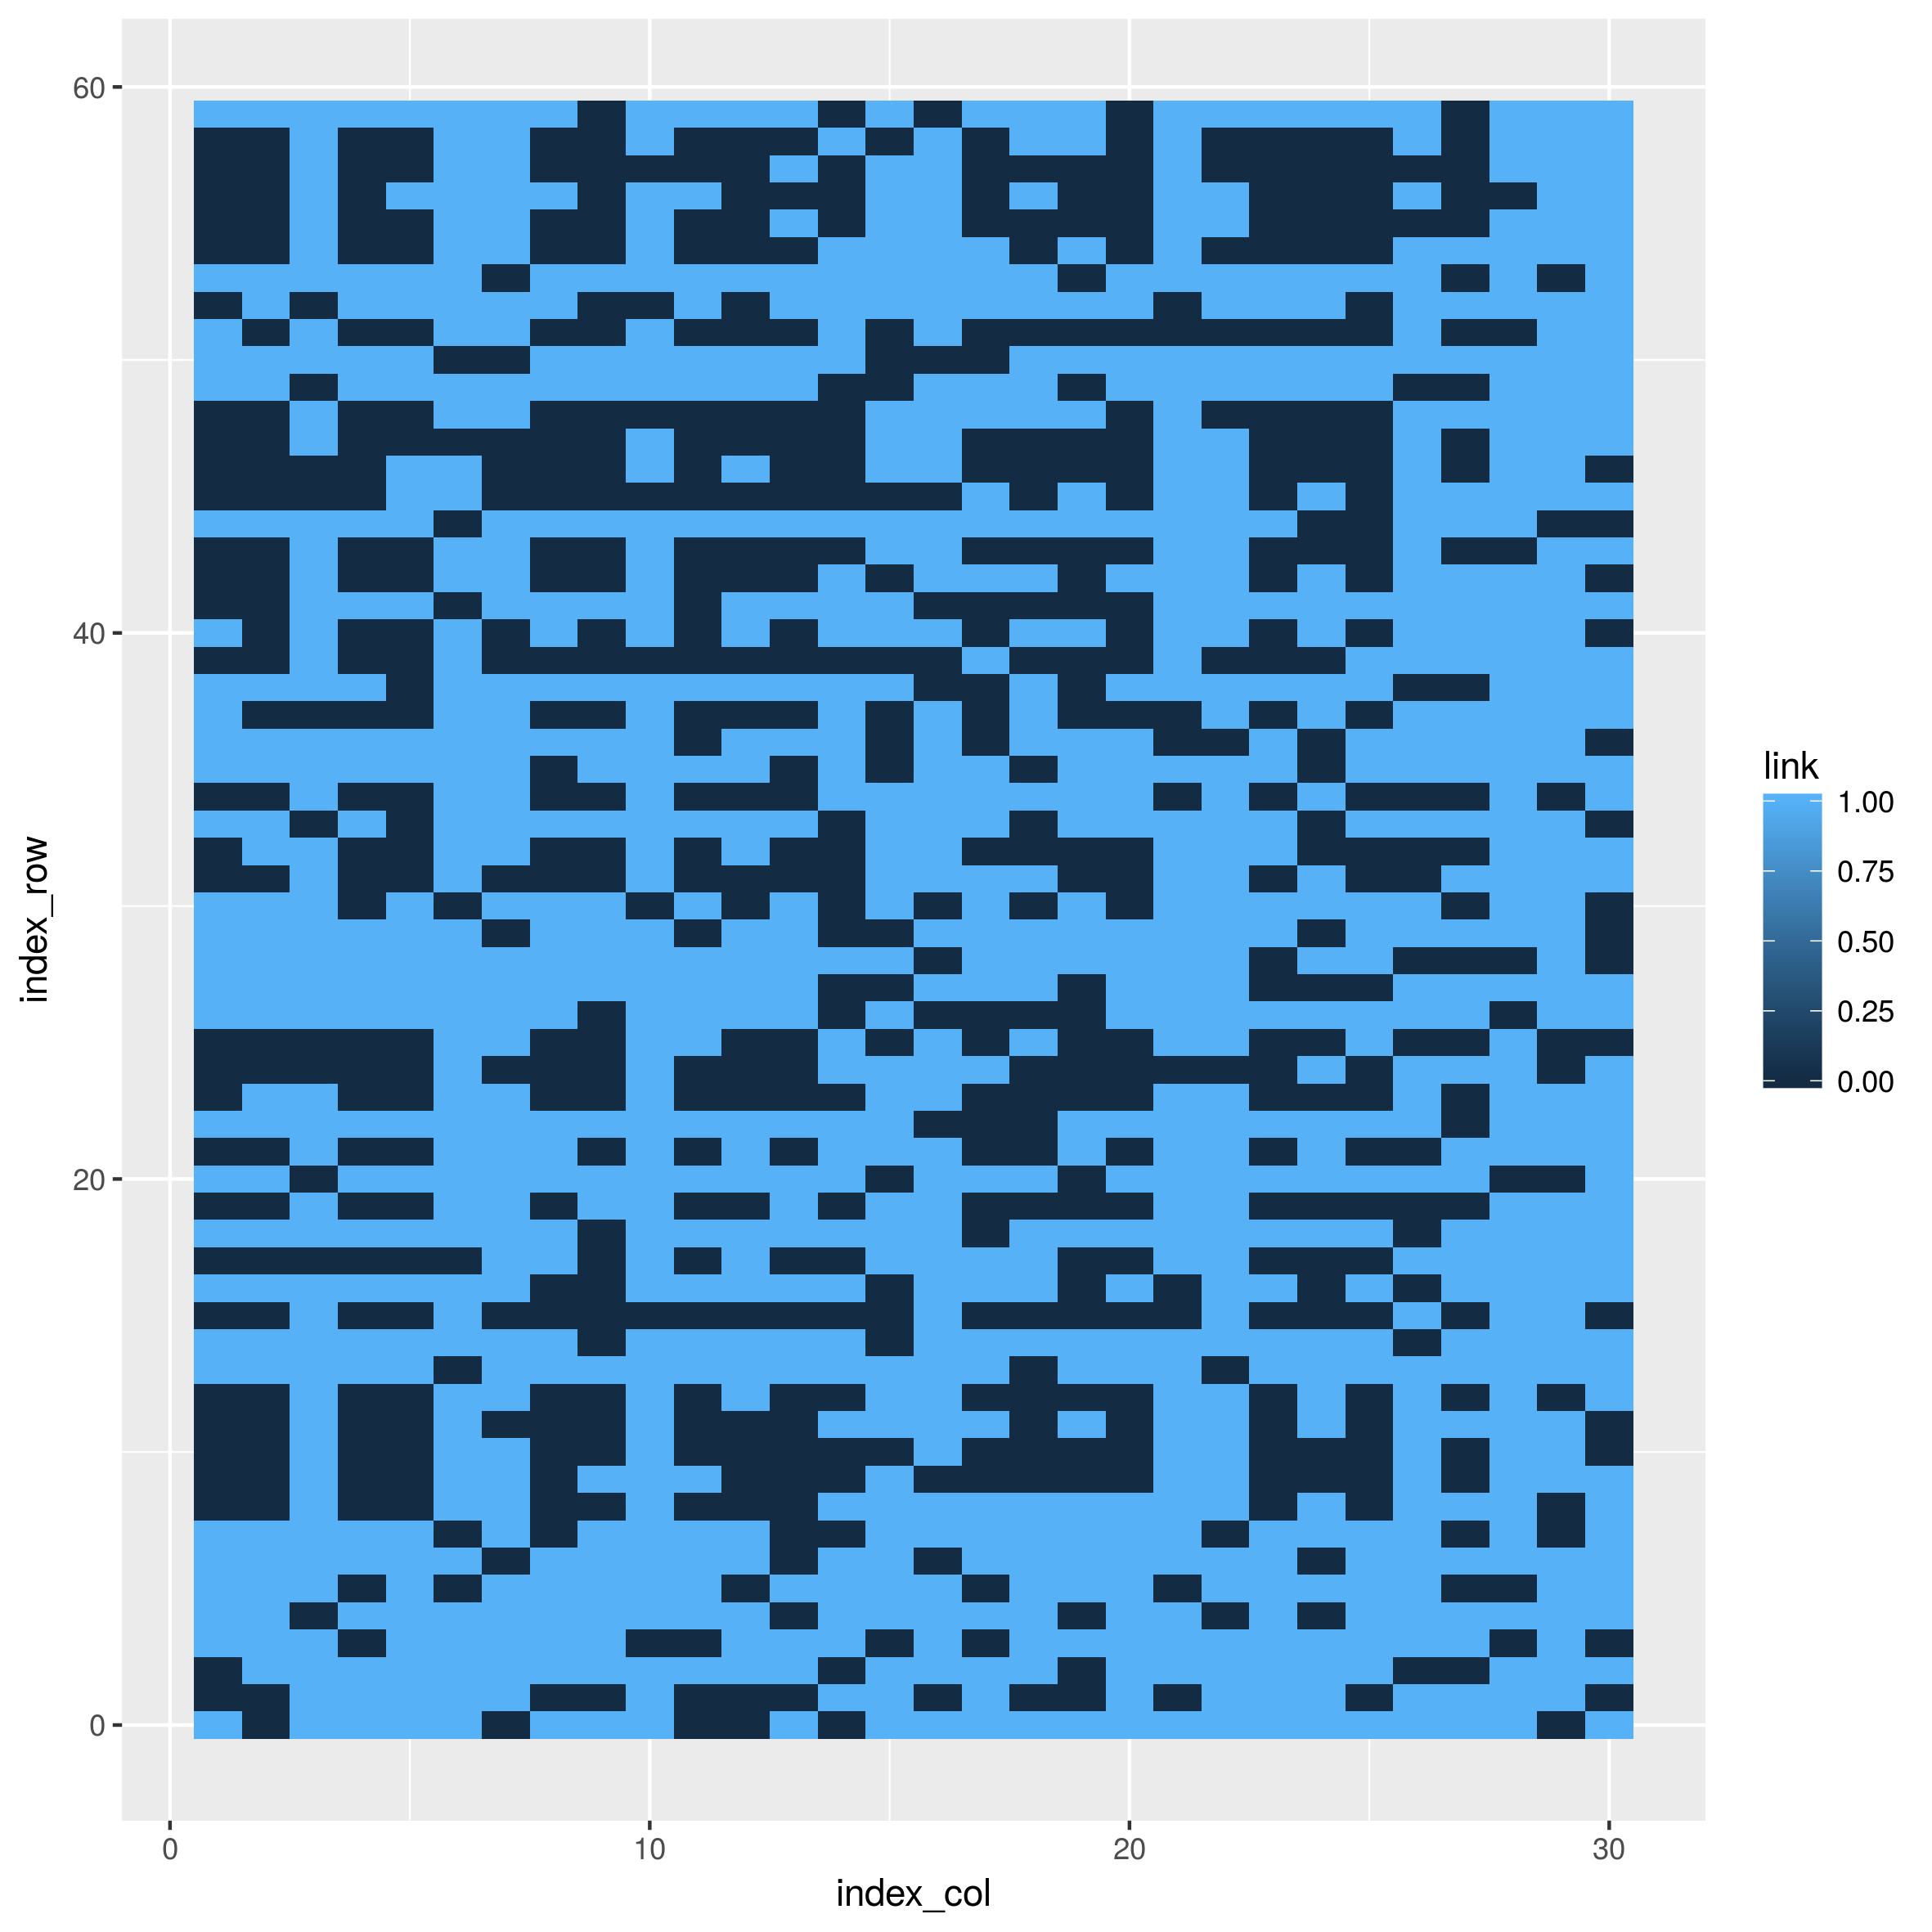
\includegraphics[scale=.2]{plots/lbm/Nested_adja.png}&
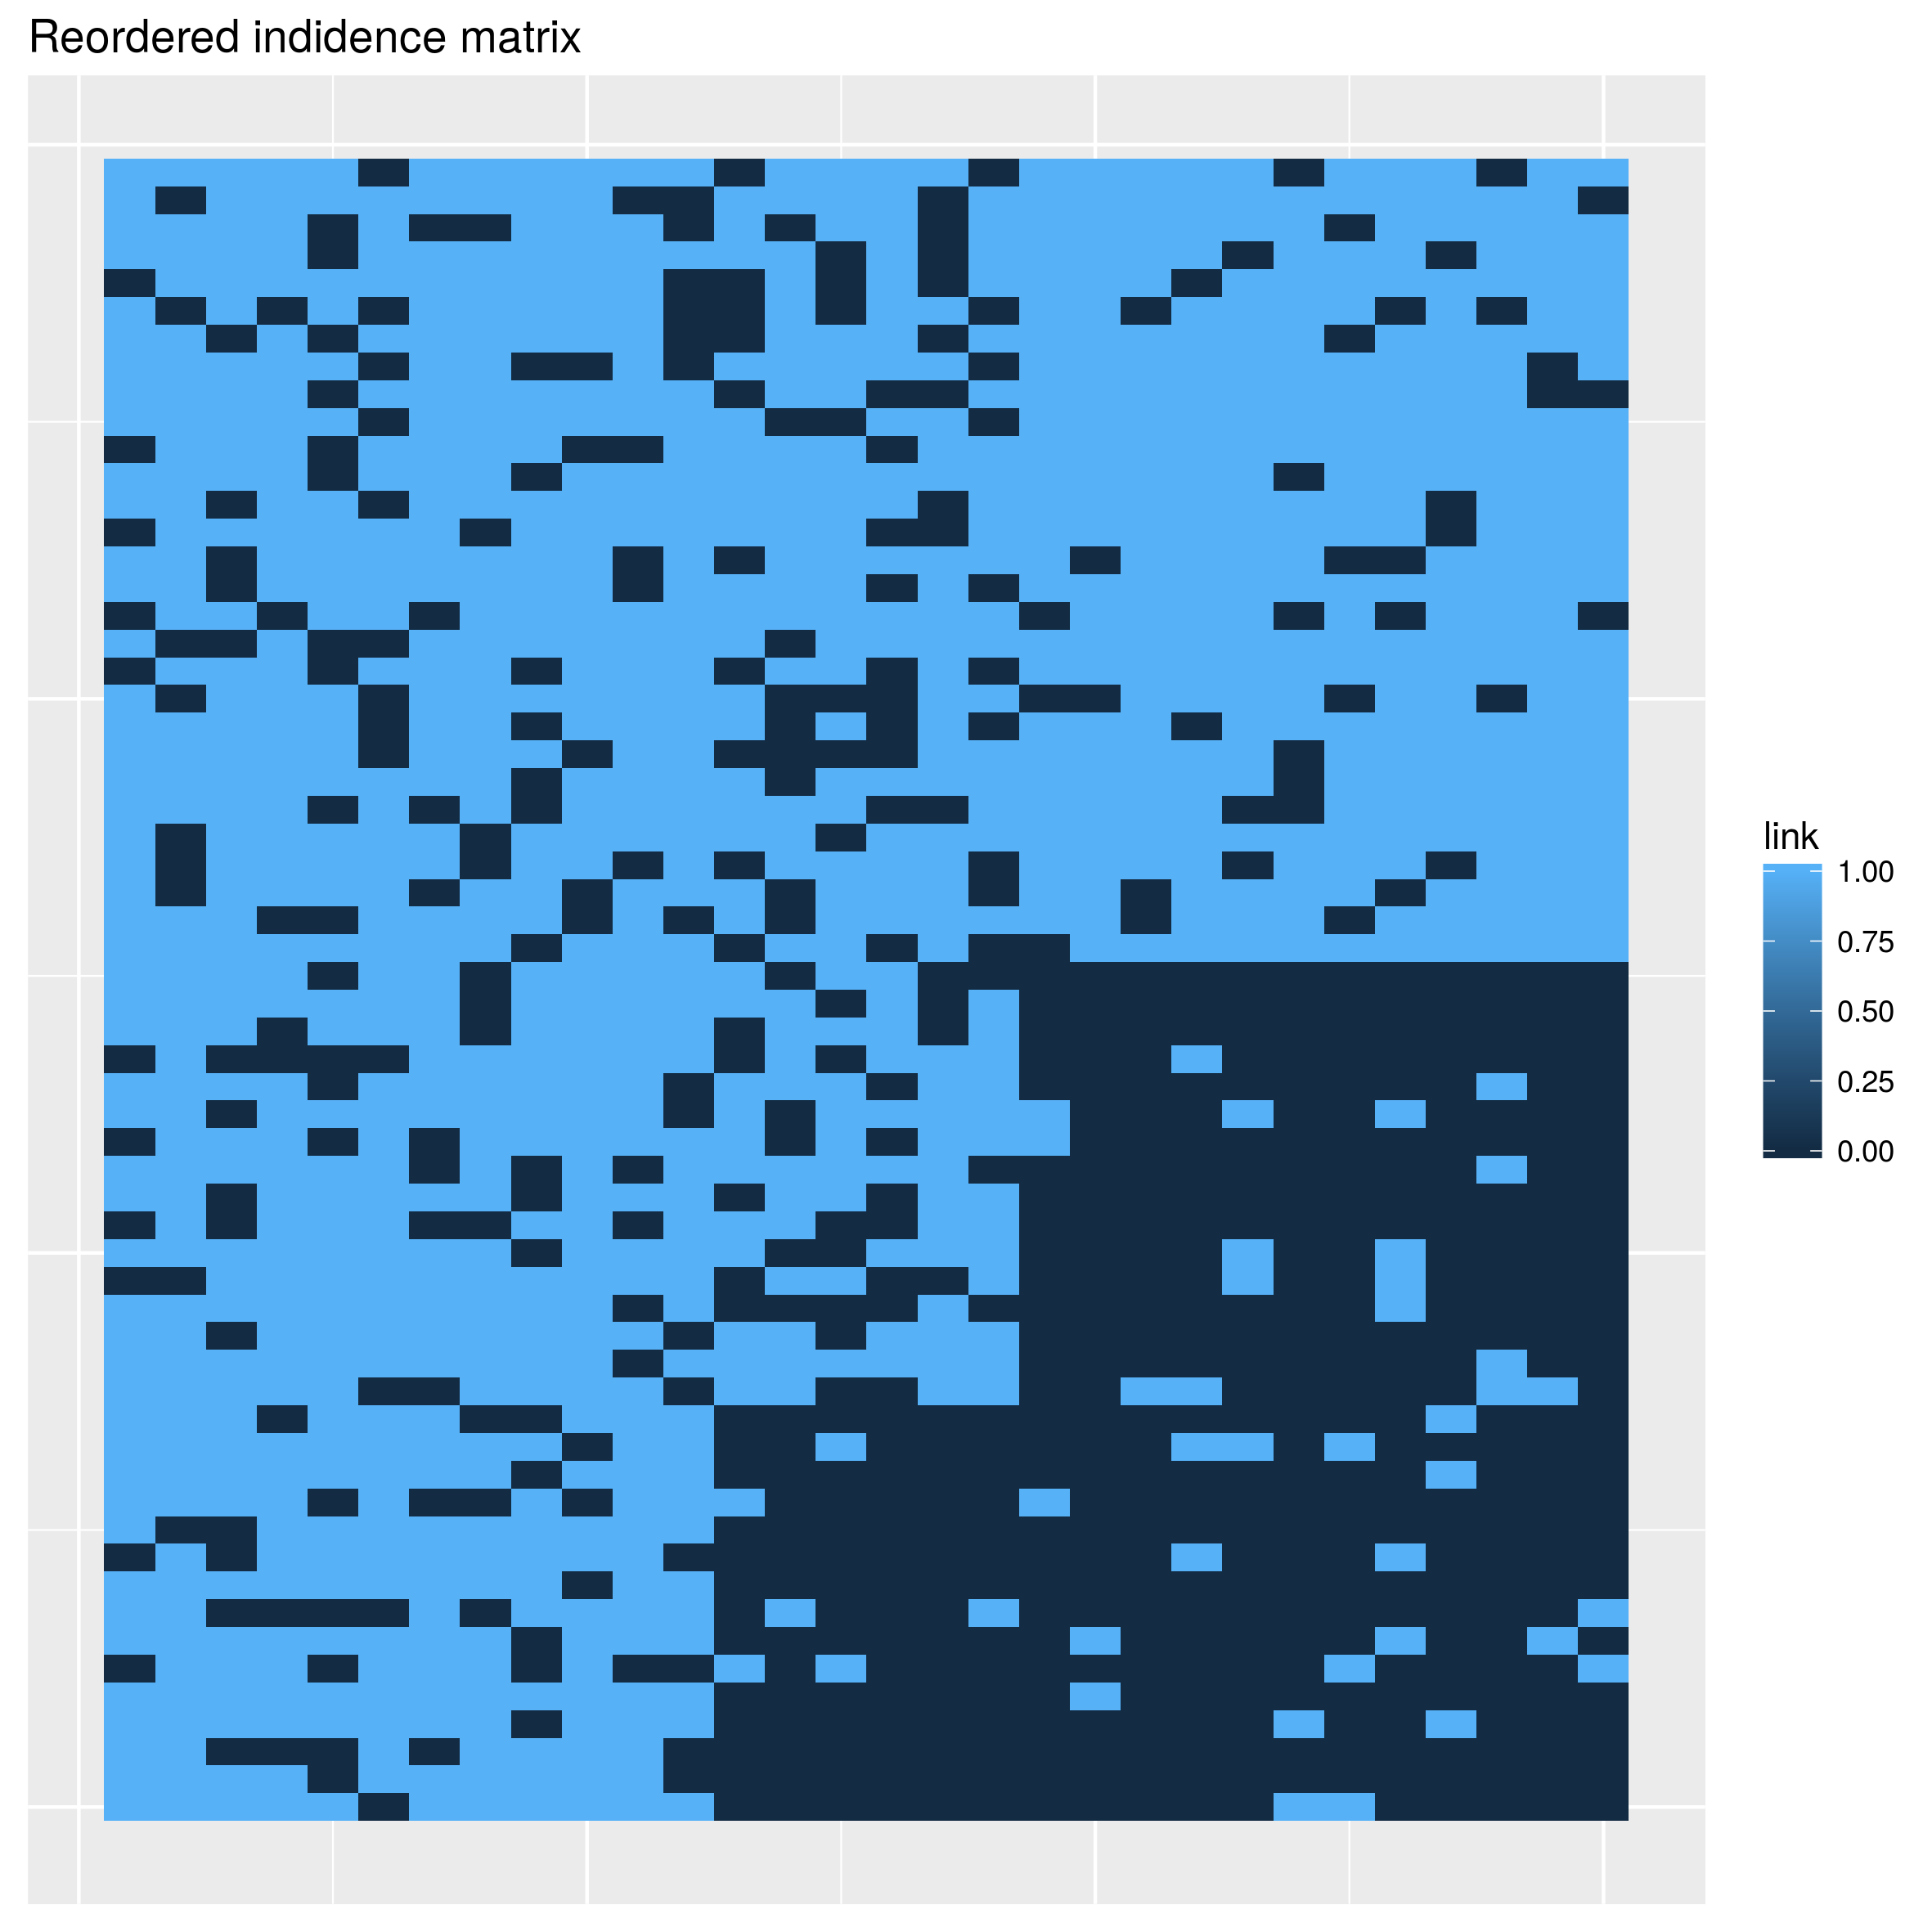
\includegraphics[scale=.2]{plots/lbm/Nested_reordered_adja_without_groups.png}
 \end{tabular}
 
 

\end{frame}



\begin{frame}
 \frametitle{LBM for ant-plant data}
 
 \begin{center}
  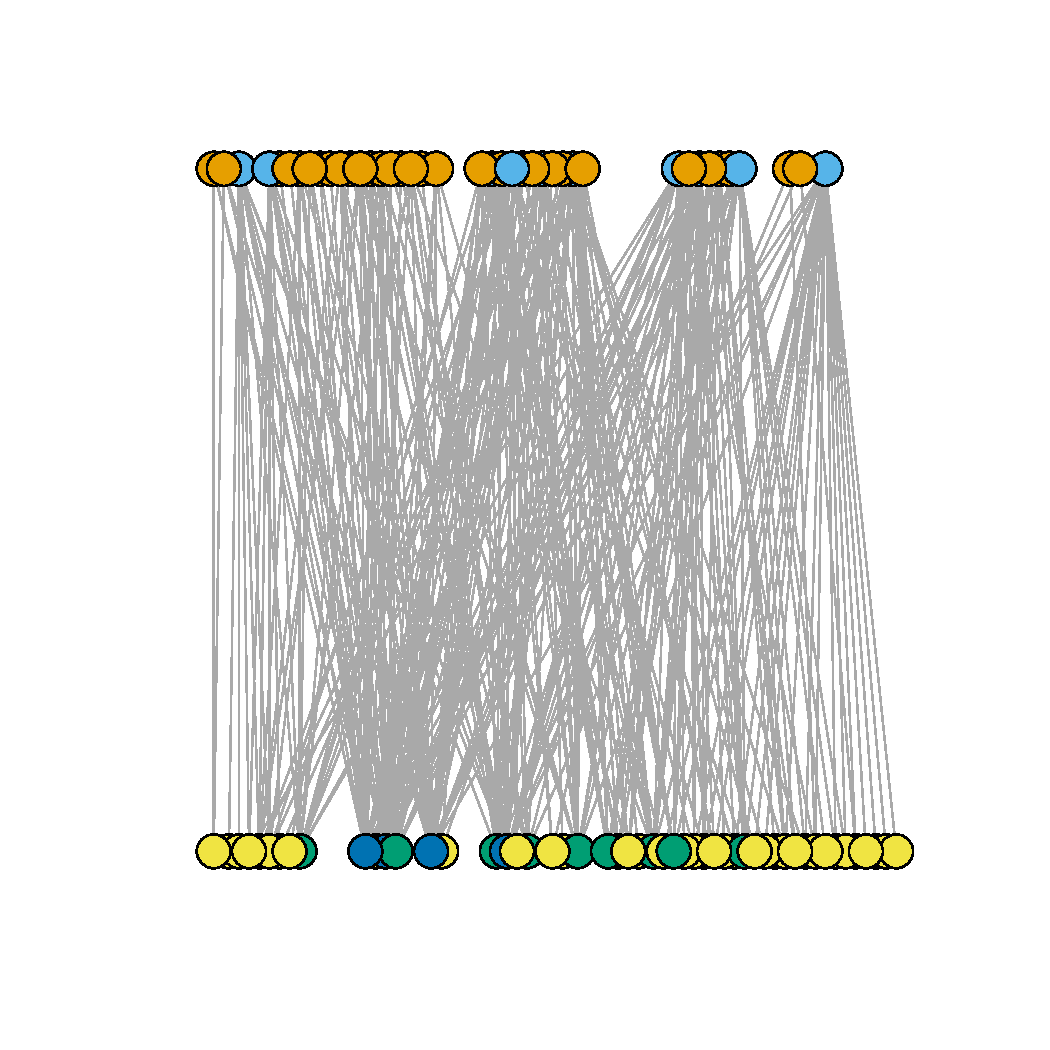
\includegraphics[scale=.3]{plots/bluthgen.pdf}
  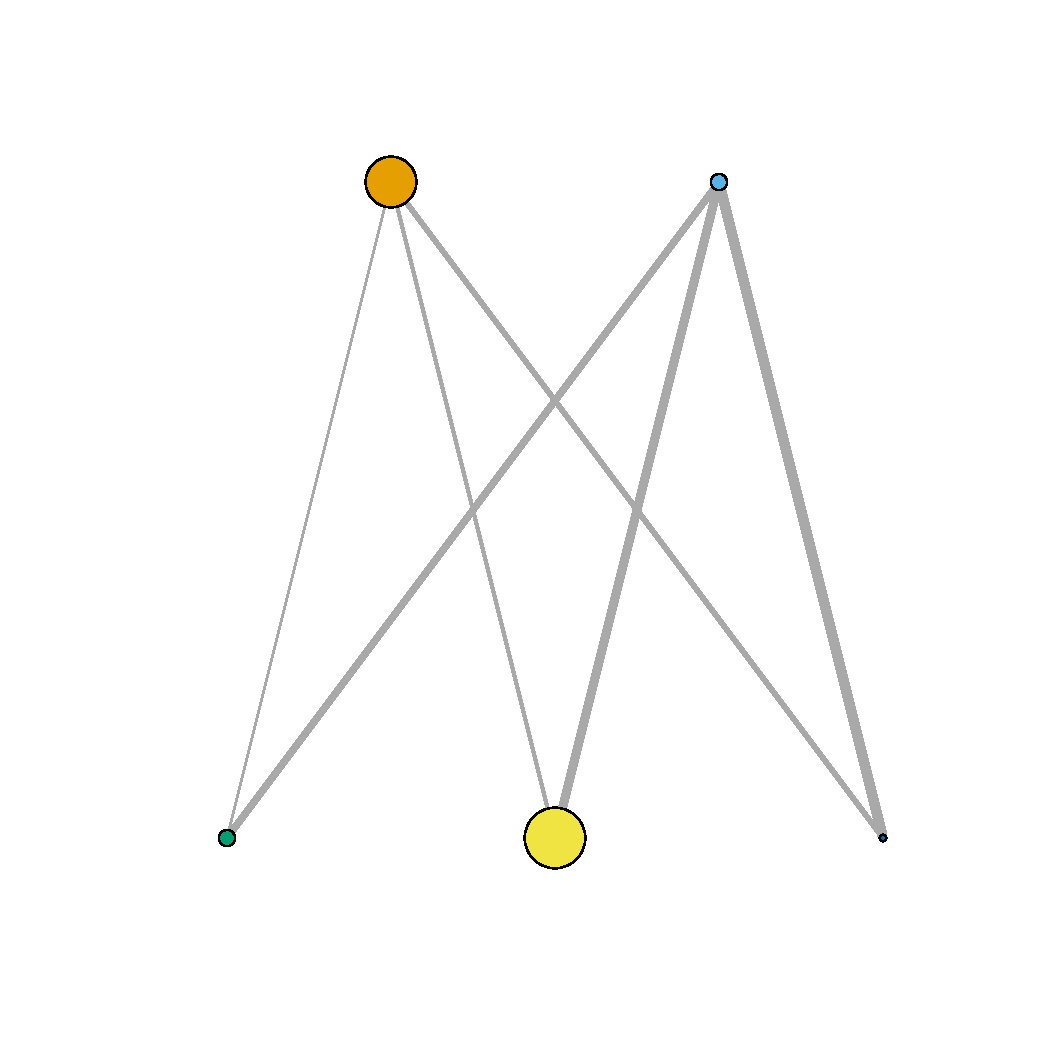
\includegraphics[scale=.3]{plots/bluthgen_sum.pdf}
 \end{center}

 \begin{itemize}
  \item 2 blocks found over the $41$ ant species,
  \item 3 blocks found over the $51$ plant species.
 \end{itemize}

\textcolor{blue}{Blüthgen, Stork \& Fiedler (2004)}

\end{frame}




\section{Some possible extensions}


\begin{frame}
 \frametitle{Valued-edge networks or multiplex-edge networks}
 
 Information on edges can be something different from presence/absence.
 It can be:
 \begin{enumerate}
  \item a count of the number of observed interactions,
  \item a quantity interpreted as the interaction strength,
  \item several kind of interactions between nodes (Multiplex networks).
 \end{enumerate}

 \bigskip
 
 
Natural extensions of SBM and LBM for these three cases:
 \begin{enumerate}
  \item Poisson distribution: $X_{ij} \ | \ \{i\in\textcolor{yellow!40!orange}{\bullet},j\in\textcolor{blue!80!black}{\bullet}\}
\sim^{\text{ind}} \mathcal{P}(\lambda_{\textcolor{yellow!40!orange}{\bullet}\textcolor{blue!80!black}{\bullet}})$,
 \item Gaussian distribution: $X_{ij} \ | \ \{i\in\textcolor{yellow!40!orange}{\bullet},j\in\textcolor{blue!80!black}{\bullet}\}
\sim^{\text{ind}} \mathcal{N}(\mu_{\textcolor{yellow!40!orange}{\bullet}\textcolor{blue!80!black}{\bullet}},\sigma^2)$,
\textcolor{blue}{Mariadassou et al. (2010)}
\item Bivariate Bernoulli: $(X_{ij},X'_{ij} )\ | \ \{i\in\textcolor{yellow!40!orange}{\bullet},j\in\textcolor{blue!80!black}{\bullet}\}
\sim^{\text{ind}} \mathcal{B}^ 2(\pi_{\textcolor{yellow!40!orange}{\bullet}\textcolor{blue!80!black}{\bullet}})$. \textcolor{blue}{
Kefi et al. (2016), Barbillon et al. (2016)} 
 \end{enumerate}

 \bigskip
\textbf{Remark:} a particular case of multiplex network is dynamic network, \textcolor{blue}{Matias \& Miele (2015)}.
 
\end{frame}


\begin{frame}
 \frametitle{Multipartite networks}

 
  
 \begin{itemize}
  \item LBM is for bipartite networks,
  \item When there are more than two functional groups involved in interactions $\Rightarrow$ Multipartite networks.

  \item  Incidence matrix
 $$X=\left(
 \begin{array}{c|c|c}
  X_1&X_2&X_3
 \end{array}
 \right)\,,$$
 where
 \begin{itemize}
  \item $X_1, X_2, X_3$ correspond to the bipartite networks with the same functional groups in rows,
  \item for instance, $X_1$ is plant-pollinator network, $X_2$ is plant-ant network and $X_3$ is plant-seed dispersers network.
 \end{itemize}

  \item Extension of LBM quite natural but choice of the number of blocks is more challenging.
  
 \end{itemize}


 


\end{frame}


% 
% \begin{frame}
% \begin{itemize}
% \item Valued edges: abundance count, weighted interactions... % ecrire de sbouts de modele
% \item multiple interactions between nodes,
% \item multipartite networks: plants, pollinator, seed dispersers, ants...
% \item Taking into account sampling conditions (through covarites...).
% \end{itemize}
% \end{frame}


\begin{frame}
 \frametitle{Taking into account covariates}
 
 Sometimes covariates are available. They may be on:
 \begin{itemize}
  \item nodes,
  \item edges,
  \item both.
 \end{itemize}

 \bigskip
 
 
 \begin{enumerate}
  \item They can be used a posteriori to explain blocks inferred by SBM.
  \item Extension of the SBM which takes into account covariates. Blocks are structure of interaction which is not 
  explained by covariates !
 \end{enumerate}

 \bigskip
 
 If covariates are sampling conditions, case 2 may more interesting.
 
\end{frame}




\begin{frame}
 \frametitle{Probabilistic model for networks in a nutshell}
 
 SBM/LBM
 \begin{itemize}
  \item generative models,
  \item flexible,
  \item comprehensive models which can be linked to a lot of classical descriptors.
  
 \end{itemize}

 \bigskip
 Extension of the binary SBM model are quite natural:
 
 \begin{itemize}
  \item all the one presented above,
  \item missing data in the network,
  \item multi-layers ?
 \end{itemize}

 
 
\end{frame}



\end{document}
